
\documentclass{article} % For LaTeX2e
\usepackage{nips14submit_e,times}


% For figures
\usepackage{graphicx} % more modern
%\usepackage{epsfig} % less modern
\usepackage{caption}
\usepackage{subcaption}
\usepackage{amsmath,amsfonts,amsthm,amssymb}
\usepackage{listings}
\usepackage{tabularx}
\usepackage{multicol}
\usepackage{float}
\usepackage[protrusion=true,expansion=true]{microtype}
\usepackage{wrapfig}
\setlength{\emergencystretch}{3em}
\usepackage[numbers]{natbib}

\usepackage{thm-restate}


\usepackage{tikz}

\usepackage{multirow}

% For algorithms
\usepackage[algoruled,vlined,linesnumbered]{algorithm2e}
%\usepackage{algorithm}
%\usepackage{algorithmic}

\usepackage{multicol}
\usepackage{comment}

% As of 2011, we use the hyperref package to produce hyperlinks in the
% resulting PDF.  If this breaks your system, please commend out the
% following usepackage line and replace \usepackage{icml2013} with
% \usepackage[nohyperref]{icml2013} above.
\usepackage{hyperref}

% Packages hyperref and algorithmic misbehave sometimes.  We can fix
% this with the following command.
\newcommand{\theHalgorithm}{\arabic{algorithm}}


\graphicspath{{figures/}}


\newcommand{\ie}{{\em i.e.,}~}
\newcommand{\eg}{{\em e.g.,}~}

%%%%%%%%%%%%%%%%%%%%%%%%%%%%%%%%%%%%%%%%%%%%%%%%%%%%%%%%%%%%%%%%%%%%%%%%%%%%%%
%% Algorithm names
\newcommand{\hogwild}{CF-2g}
\newcommand{\occ}{CC-2g}
\newcommand{\seqalg}{Seq-2g}
\newcommand{\hogwildshort}{CF}
\newcommand{\occshort}{CC}
\newcommand{\seqalgshort}{Seq}
%%%%%%%%%%%%%%%%%%%%%%%%%%%%%%%%%%%%%%%%%%%%%%%%%%%%%%%%%%%%%%%%%%%%%%%%%%%%%%

\begingroup
    \makeatletter
    \@for\theoremstyle:=definition,remark,plain\do{%
        \expandafter\g@addto@macro\csname th@\theoremstyle\endcsname{%
            \addtolength\thm@preskip\parskip
            }%
        }
\endgroup
\newtheorem{dfn}{Definition}[section]
\newtheorem{thm}{Theorem}[section]
\newtheorem{cor}[thm]{Corollary}
\newtheorem{lem}[thm]{Lemma}
\newtheorem{prop}[thm]{Proposition}
\newtheorem{exmp}[thm]{Example}
\newtheorem{claim}{Claim}

\floatstyle{ruled}
\newfloat{program}{thp}{lop}
\floatname{program}{Program}

\newenvironment{denseitemize}{
\begin{itemize}[topsep=2pt, partopsep=0pt, leftmargin=1.5em]
  \setlength{\itemsep}{4pt}
  \setlength{\parskip}{0pt}
  \setlength{\parsep}{0pt}
}{\end{itemize}}

\newenvironment{packed_enum}{
\begin{enumerate}
  \setlength{\itemsep}{4pt}
  \setlength{\parskip}{0pt}
  \setlength{\parsep}{0pt}
}{\end{enumerate}}




\lstdefinelanguage{scala}{
  morekeywords={abstract,case,catch,class,def,%
    do,else,extends,false,final,finally,%
    for,if,implicit,import,match,mixin,%
    new,null,object,override,package,%
    private,protected,requires,return,sealed,%
    super,this,throw,trait,true,try,%
    type,val,var,while,with,yield},
  otherkeywords={=>,<-,<\%,<:,>:,\#,@},
  sensitive=true,
  morecomment=[l]{//},
  morecomment=[n]{/*}{*/},
  morestring=[b]",
  morestring=[b]',
%  numbers=left,
  morestring=[b]"""
}



% Commenting system
\newcommand{\Comments}{1}
\newcommand{\note}[2]{\ifnum\Comments=1\textcolor{#1}{#2}\fi}
\newcommand{\xinghao}[1]{\note{red}{[XP: #1]}}
\newcommand{\joey}[1]{\note{blue}{[JG: #1]}}
\newcommand{\stef}[1]{\note{green}{[SJ: #1]}}
\newcommand{\joseph}[1]{\note{cyan}{[JB: #1]}}

\newcommand{\argmin}{\operatornamewithlimits{argmin}}






%% ---------------------------------------------------------
%% Terminology
\newcommand{\term}[1]{\textbf{#1}}


%% ---------------------------------------------------------
%% Citation/Reference commands
\newcommand{\citecf}[1]{(\cf, \cite{#1})}
\newcommand{\tableref}[1]{Table~\ref{#1}}
\newcommand{\figref}[1]{Fig.~\ref{#1}}
\newcommand{\listref}[1]{Listing~\ref{#1}}

\newcommand{\eqnref}[1]{Eq.~(\ref{#1})}
\newcommand{\secref}[1]{Sec.~\ref{#1}}
\newcommand{\chapref}[1]{Chapter~\ref{#1}}

\newcommand{\dfnref}[1]{Definition~\ref{#1}}
\newcommand{\thmref}[1]{Thm.~\ref{#1}}
\newcommand{\propref}[1]{Prop.~\ref{#1}}
\newcommand{\lemref}[1]{Lem~\ref{#1}}
\newcommand{\exmpref}[1]{Example~\ref{#1}}
\newcommand{\corref}[1]{Cor.~\ref{#1}}
\newcommand{\algref}[1]{Alg.~\ref{#1}}
\newcommand{\procref}[1]{Proc.~\ref{#1}}
\newcommand{\alglineref}[1]{Line~\ref{#1}}
\newcommand{\probref}[1]{Problem~(\ref{#1})}
\newcommand{\appendref}[1]{Appendix~\ref{#1}}

%% ---------------------------------------------------------
%% Basic Math
\newcommand{\abs}[1]{\left|#1\right|}
\newcommand{\ceil}[1]{\left\lceil #1 \right\rceil}
\newcommand{\floor}[1]{\left\lfloor #1 \right\rfloor}


%% ---------------------------------------------------------
%% special math functions
\newcommand{\polylog}[2]{\,\mathbf{Li}_{#1}\left( #2 \right)}
\newcommand{\harmonic}[2]{\,\mathbf{h}_{#1}\left( #2 \right)}

%% ---------------------------------------------------------
%% Norms
\newcommand{\Lone}{L_{1}}
\newcommand{\Linf}{L_{\infty}}
\newcommand{\LInfNorm}[1]{\left|\left| #1 \right|\right|_{\infty}}
\newcommand{\LOneNorm}[1]{\left|\left| #1 \right|\right|_1}

\newcommand{\hinge}[1]{\left[  #1 \right]_+}

%% ---------------------------------------------------------
%% Probability notation
\newcommand{\given}{\,|\,}
\newcommand{\stdist}[1]{\mathbf{\pi} \left( #1 \right) }
\newcommand{\Prb}[1]{\mathbf{P} \left( #1 \right) }
\newcommand{\PrbEst}[1]{\mathbf{\tilde{P}} \left( #1 \right) }
\newcommand{\Ent}[1]{\mathbf{H} \left( #1 \right) }
\newcommand{\PiPrb}[1]{\Prb{ #1 } }
\newcommand{\Kern}[1]{K \left( #1 \right) }
\newcommand{\Ex}[1]{\mathbf{E} \left[ #1 \right] }
\newcommand{\Exwrt}[2]{\mathbf{E}_{#1} \left[ #2 \right] }
\newcommand{\Variance}[1]{\mathbf{Var} \left[ #1 \right] }
\newcommand{\Ind}[1]{\mathbf{1}\left[ #1 \right]}
\newcommand{\Bern}[1]{\text{Bern}( #1 ) }

%% ---------------------------------------------------------
%% Set notation
\newcommand{\reals}{\mathbb{R}}
\newcommand{\integers}{\mathbb{Z}}
\newcommand{\set}[1]{\left\{#1\right\}}
\newcommand{\vecspace}{\mathcal{V}}
\newcommand{\Union}{\bigcup}
\newcommand{\Inter}{\bigcap}
\newcommand{\union}{\cup}
\newcommand{\inter}{\cap}
\newcommand{\size}[1]{\left| #1 \right|}


%% ---------------------------------------------------------
%% Complexity
\newcommand{\BigO}[1]{O\hspace{-1pt}\left( #1 \right)}
\newcommand{\BigTheta}[1]{\Theta \left( #1 \right)}
\newcommand{\BigOmega}[1]{\Omega \left( #1 \right)}





%% ---------------------------------------------------------
%% Algorithms
\SetKwFor{ParForAll}{for}{do in parallel}{end}
\SetKwFunction{Map}{Map}
\SetKwFunction{Reduce}{Reduce}

\SetKwInput{Input}{Input}
\SetKwInput{Output}{Output}
\SetKwInput{SideEffect}{SideEffect}
\SetKwInput{Define}{Define}
\SetKwInput{Global}{Global}
\SetKwFor{DoWithProbability}{with probability}{}{}
\SetKwFunction{DPMeansOp}{DPMeansOp}
\SetKwFunction{DPValidate}{DPValidate}
\SetKwFunction{OFLValidate}{OFLValidate}
\SetKwFunction{BPMeansOp}{BPMeansOp}
\SetKwFunction{BPValidate}{BPValidate}
\SetKwFunction{NewClusters}{AcceptedClusters}

\SetKw{WaitUntil}{wait until}

\SetKwFunction{Mean}{Mean}
\SetKwFunction{Ref}{Ref}


%% ---------------------------------------------------------
%% Paper specific notation

% All the data
\newcommand{\data}{\mathcal{D}}
% \datablock{machine}
\newcommand{\datablock}[1]{\data_{#1}}

\newcommand{\clusters}{\mathcal{C}}
\newcommand{\gclusters}{\hat\clusters}
\newcommand{\newclusters}{\tilde\clusters}
% local clusters \lclusters{machine}
\newcommand{\lclusters}[1]{\clusters_{#1}}

%\newcommand{\bregd}[2]{D_\phi\left(#1,#2\right)}
\newcommand{\bregd}[2]{\left\|#1-#2\right\|}


% for ofl analysis:
\newcommand{\CFL}{C^{\text{FL}}}
\newcommand{\muFL}{\mu^{\text{FL}}}



\makeatletter
\newcommand\footnoteref[1]{\protected@xdef\@thefnmark{\ref{#1}}\@footnotemark}
\makeatother




\title{Parallel Double Greedy Submodular Maximization}

\author{
Xinghao Pan$^1$ Joseph Gonzalez$^1$ Stefanie Jegelka$^1$ Joseph Bradley$^{1}$ Michael I. Jordan$^{1,2}$\\
$^1$Department of Electrical Engineering and Computer Science, and $^2$Department of Statistics\\
University of California, Berkeley\\
Berkeley, CA USA 94720\\
  \texttt{\{xinghao,jegonzal,stefje,tab,?\}@eecs.berkeley.edu} \\
}

% \address{University of California
% 465 Soda Hall, MC-1776
% Berkeley, CA 94720-1776}

\newcommand{\fix}{\marginpar{FIX}}
\newcommand{\new}{\marginpar{NEW}}


%\nipsfinalcopy

\begin{document}


\maketitle


\begin{abstract}
Many machine learning problems can be reduced to the maximization of  submodular functions.
Although well understood in the serial setting, the parallel maximization of submodular functions remains an open area of research with recent results \cite{Mirzasoleiman2013} only addressing monotone functions.
The optimal algorithm for maximizing the more general class of non-monotone submodular functions was introduced by \citet{buchbinder2012} and follows a strongly serial double-greedy logic and program analysis.
In this work, we propose two methods to parallelize the double-greedy algorithm.
% bridge this gap and make the theoretical benefits available in a scalable setting.
% % between those theoretical benefits and scalable computing.
% We propose and analyze two parallel double greedy algorithms.
The first, \emph{coordination-free} approach emphasizes speed at the cost of a weaker approximation guarantee.
The second, \emph{concurrency control} approach guarantees a tight 1/2-approximation, at the quantifiable cost of additional coordination and reduced parallelism.
As a consequence we explore the trade-off space between guaranteed performance and objective optimality.
% We bound both the weaker approximation factor and the reduction in parallelism.
We implement and evaluate both algorithms on multi-core hardware and billion edge graphs, demonstrating both the scalability and tradeoffs of each approach.
%
%Many machine learning problems can be reduced to the maximization of a submodular function.
%Recently, \citet{buchbinder2012} achieved a tight 1/2-approximation for unconstrained submodular maximization using a double greedy algorithm.
%Unfortunately, the double greedy algorithm was developed and analyzed in the serial setting limiting our ability to leverage parallel hardware.
%In this work we propose and analyze two parallel extensions to the \cite{buchbinder2012} double greedy algorithm.
%The first, \emph{coordination-free} approach emphasizes speed at the cost of a weaker approximation guarantee.
%The second, \emph{concurrency control} approach guarantees the same tight 1/2-approximation, at the cost of additional coordination and reduced parallelism.
%We bound both the weaker approximation factor and the reduction in parallelism.
%We implement and evaluate both algorithms on multi-core hardware and billion edge graphs demonstrating both the scalability and tradeoffs of each approach.
%
% Many machine learning problems can be formulated as maximization of submodular functions. \cite{buchbinder2012} recently proposed a double greedy algorithm for unconstrained submodular maximization that achieves a tight 1/2-approximation. However, double greedy is an inherently sequential, linear time algorithm that does not scale to big data.

% We present two approaches to extend the double greedy algorithm to a parallel setting.
% The first, `coordination-free' approach emphasizes speed at the cost of a weaker approximation guarantee -- it achieves a $(1/2 - O(1/N))$ approximation for max cut on a complete graph.
% The second, `concurrency control' approach guarantees the same tight 1/2-approximation, at the cost of greater coordination.

% Our parallel algorithms scale well on synthetic and real datasets, and suffer little or no loss of objective value compared to the sequential algorithm.
\end{abstract}

\section{Introduction}



Many important problems including sensor placement \cite{krauseGuestrin11}, image co-segmentation \cite{kim11}, MAP inference for determinantal point processes \cite{gillenwater12}, influence maximization \cite{kkt03}, and document summarization \cite{lin11} may be expressed as the maximization of a submodular function.
The submodular formulation enables the use of targeted algorithms \cite{buchbinder2012,nemhauser1978} that offer theoretical worst-case guarantees on the quality of the solution.
For several maximization problems of \emph{monotone} submodular functions (satisfying $F(A) \leq F(B)$ for all $A \subseteq B$), a simple greedy algorithm \cite{nemhauser1978} achieves the optimal approximation factor of $1-\frac{1}{e}$.
The optimal result for the wider, important class of \emph{non-monotone} functions  -- an approximation guarantee of $1/2$ --  is much more recent, and achieved by a \emph{double greedy} algorithm by \citet{buchbinder2012}.


While these algorithms are both theoretically optimal and perform well in practice, their design is inherently serial, limiting their scalability to large problem instances and advances in parallel hardware.
% Increasingly often, real-world applications demand
% % one wishes
% to solve the above-mentioned problems at very large scale.
This limitation raises the question of parallel algorithms for submodular maximization that ideally preserve the theoretical bounds, or weaken them gracefully, in a quantifiable manner.


In this paper, we study the parallelization of greedy algorithms, in particular the double greedy algorithm, from the perspective of \emph{parallel transaction processing systems}.
This alternative perspective allows us to apply advances in database research ranging from fast coordination free approaches with limited guarantees to sophisticated concurrency control techniques which ensure a direct correspondence between parallel and serial executions at the expense of increased coordination. % cost of slightly reduced performance.


By exploiting the exchangeability of the greedy ordering and the sparsity of  the submodular functions we develop two parallel algorithms for the maximization of non-monotone submodular functions.
We propose \hogwild{} as a coordination free double greedy algorithm and characterize the effect of reduced coordination on the approximation ratio.
By bounding the possible outcomes of concurrent transactions we introduce the \occ{} algorithm which guarantees serializable parallel execution and retains the optimality of the double greedy algorithm at the expense of increased coordination.


The primary contributions of this paper are:
\begin{enumerate}
\item We propose two parallel algorithms for unconstrained non-monotone submodular maximization, which trade-off parallelism and tight approximation guarantees.
\item We prove that \occ{} produces an outcome equivalent to the sequential double greedy algorithm, thus preserving the tight 1/2-approximation guarantee.
\item We analytically bound the amount of coordination of \occ{} for set-cover and max-cut.
\item We provide approximation guarantees for \hogwild{} and analytically bound the expected loss in objective value for set-cover and max-cut.
\item We demonstrate empirically using two synthetic and three real datasets that our parallel algorithms perform well in terms of both speed and objective values.
\end{enumerate}

The rest of the paper is organized as follows.
\secref{sec:submodularmax} discusses the problem of submodular maximization and introduces the double greedy algorithm.
\secref{sec:concurrencycontrol} provides background on concurrency control mechanisms.
We describe and provide intuition for our \hogwild{} and \occ{} algorithms in \secref{sec:alghogwild} and \secref{sec:algocc}, and then analyze the algorithms both theoretically (\secref{sec:analysis}) and empirically (\secref{sec:evaluation}).
%\secref{sec:analysis} analyzes the parallel algorithms.
%Both algorithms are evaluated in \secref{sec:evaluation}, and we conclude with related work and discussions in \secref{sec:related} and \secref{sec:discussions}.














\section{Submodular Maximization \label{sec:submodularmax}}
A set function $F: 2^V \to \mathbb{R}$ defined over subsets of a ground set $V$ is \emph{submodular} if it satisfies \emph{diminishing marginal returns}: for all $A \subseteq B \subseteq V$ and  $e \notin V$, it holds that $F(A \union \{e\}) - F(A) \geq F(B \union \{e\}) - F(B)$. Throughout this paper, we will assume that $F$ is nonnegative and $F(\emptyset)=0$.
Submodular functions have emerged in areas such as game theory \cite{shapley71}, graph theory \cite{frank93}, combinatorial optimization \cite{schrijver02}, %stochastic processes \cite{},
and machine learning \cite{tutorial,tutorial2}.
Casting machine learning as submodular optimization enables the use of algorithms for submodular maximization \cite{buchbinder2012,nemhauser1978} that offer theoretical worst-case guarantees on the quality of the solution.
%Problems like as sensor placement \cite{krauseGuestrin11}, image co-segmentation \cite{kim11}, MAP inference with determinantal point process priors \cite{gillenwater12}, influence maximization \cite{kkt03} or document summarization \cite{lin11} may be phrased as the maximization of a submodular function, which enables the use of algorithms for submodular maximization \cite{buchbinder2012,nemhauser1978} that offer theoretical worst-case guarantees on the quality of the solution.

While those algorithms confer strong guarantees and tend to work very well in practice, their design is inherently serial.
% But increasingly often, one wishes to solve the above-mentioned problems at very large scale. This development raises the question of parallel algorithms for submodular maximization that ideally preserve the theoretical bounds, or weaken them gracefully, in a quantifiable manner.
%
Recent work has addressed faster \cite{badan14,wei14} and parallel \cite{Mirzasoleiman2013,kumar13} versions of the greedy algorithm by \citet{nemhauser1978} for maximizing \emph{monotone} submodular functions that satisfy $F(A) \leq F(B)$ for any $A \subseteq B \subseteq V$.
However, many important applications in machine learning lead to \emph{non-monotone} submodular functions.
For example, graphical model inference \cite{gillenwater12,reed13}, or trading off any submodular gain maximization with costs (functions of the form $F(S) = G(S) - \lambda M(S)$, where $G(S)$ is monotone submodular and $M(S)$ a linear (modular) cost function), such as for utility-privacy tradeoffs \cite{krause10priv},
%and feature selection with a modular cost function \joey{Is there a better example or at least a citation?}
 require maximizing non-monotone submodular functions.
% and when trading off gains with (linear) cost functions (functions of the form $F(S) = G(S) + \lambda M(S)$, where $G(S)$ is monotone submodular and $M(S)$ is a linear (modular) cost function), we aim to maximize a \emph{non-monotone} submodular function.
For non-monotone functions, the simple greedy algorithm in \cite{nemhauser1978} can perform arbitrarily poorly (see Appendix~\ref{app:greedyfail} for an example).
Intuitively, the introduction of additional elements with monotone submodular functions never decreases the objective while introducing elements with non-monotone submodular functions can \emph{decrease} the objective to its minimum.
% Intuitively, for monotone functions including more elements eventually neither helps nor hurts, while for non-monotone functions it can hurt to the extent of reducing the function value back to zero.
For non-monotone functions, \citet{buchbinder2012} recently proposed an optimal double greedy algorithm that works well in a serial setting. In this paper, we study parallelizations of this algorithm.

% they develop and analyze in a serial setting. Here, we theoretically and empirically study parallel analogs of this algorithm.

\paragraph{The sequential double greedy algorithm.}
The sequential double greedy algorithm of \citet{buchbinder2012} (\seqalg{}, in \algref{alg:submax}) maintains two sets $A^i \subseteq B^i$.
Initially, $A^0 = \emptyset$ and $B^0 = V$.
In iteration $i$, the set $A^{i-1}$ contains the items selected before item/iteration $i$, and $B^{i-1}$ contains $A^i$ and the items that are so far undecided.
The algorithm sequentially passes through the items in $V$ and determines online whether to keep item $i$ (add to $A^i$) or discard it (remove from $B^i$), based on a threshold that trades off the gain $\Delta_+(i) = F(A^{i-1} \union i) - F(A^{i-1})$ of adding $i$ to the currently selected set $A^{i-1}$, and the gain $\Delta_-(i) = F(B^{i-1}\setminus i) - F(B^{i-1})$ of removing $i$ from the candidate set, estimating its complementarity to other remaining elements.
% The decision depends on the gain of $i$ with respect to $A^i$, and the gain of removing $i$ from $B^i$.
% If the submodular function is monotone, then the double greedy algorithm essentially becomes a randomized version of the well-known greedy algorithm for monotone functions \citep{nemhauser1978}.
%Describe the double greedy algorithm:
%The sequential double greedy \cite{buchbinder2012} algorithm monotonically grows $A^i$ and shrinks $B^i$.









\section{Concurrency Patterns for Parallel Machine Learning \label{sec:concurrencycontrol}}

In this paper we adopt a transactional view of the program state and explore parallelization strategies through the lens of parallel transaction processing systems.
We recast the program state, the sets $A$ and $B$, as data, and the operations, adding elements to $A$ and removing elements from $B$, as transactions.
More precisely we reformulate the double greedy algorithm (\algref{alg:submax}) as a series of \emph{exchangeable}, \emph{Read-Write} transactions of the form:
\begin{equation}
T_e(A,B) \triangleq
\begin{cases}
   (A \union e, B) & \text{if } u_e \leq \frac{\hinge{\Delta_+(A,e)}}{ \hinge{\Delta_+(A,e)} + \hinge{\Delta_-(B,e)}}  \\
   (A, B \backslash e) & \text{otherwise. }
  \end{cases}
  \label{eqn:greedytransaction}
\end{equation}
The transaction $T_e$ is a function from the sets $A$ and $B$ to new sets $A$ and $B$ based on the element $e \in V$ and the predetermined random bits $u_e$ for that element.
To eliminate exogenous ordering effects, we associate the source of randomness with each element in the set.
% to simplify the presentation. % as $T_e$ becomes a deterministic function.


By composing the transactions $T_n (T_{n-1}(\ldots T_1(\emptyset, V)))$ we recover the serial double-greedy algorithm defined in \algref{alg:submax}.
In fact, any ordering of the \emph{serial} composition of the transactions recovers a permuted execution of \algref{alg:submax} and therefore the optimal approximation algorithm.
However, this raises the question: \emph{is it possible to apply transactions in parallel?}
If we execute transactions $T_i$ and $T_j$, with $i \neq j$, in parallel we
need a method to merge the resulting program states.
In the context of the double greedy algorithm, we could define the parallel execution of two transactions as:
\begin{equation}
T_i(A,B) + T_j(A,B) \triangleq \left(T_i(A,B)_A \union T_j(A,B)_A,  \,\, T_i(A,B)_B  \inter T_j(A,B)_B \right).
\label{eqn:merge}
\end{equation}
the union of the resulting $A$ and the intersection of the resulting $B$.
While we can easily generalize \eqnref{eqn:merge} to many parallel transactions, we cannot always guarantee that the result will corresponds to a serial composition of transactions.
As a consequence, we cannot directly apply the analysis of Buchbinder et al.~\cite{buchbinder2012} to derive strong approximation guarantees for the parallel execution.

Fortunately, several decades of research~\citep{Ozsu07,kung1981:occ} in database systems have explored efficient parallel transaction processing.
In this paper we adopt a bounded optimistic approach to parallel transaction processing in which parallel transactions are constructed under bounds on the possible program state.
If the transaction could violate the bound then it is processed serially on the server.
By adjusting the definition of the bound we can span a space of coordination free to serializable executions.




% These systems span a space ranging from extremely fast coordination free approaches which provide minimal guarantees on the composition of transactions to sophisticated concurrency control techniques which ensure a direct correspondence between parallel and serial executions at the cost of slightly reduced performance.




% A common technique is to introduce a validation stage that detects inconsistent transactions and prescribes a compensating action.
% In \algref{alg:generalparallel} we describe a general validation based meta-algorithm that we extend in subsequent sections.
% Each processor extracts a next element to process and a consistent but potentially out of data snapshot of the program state.
% Based on the snapshop and selected element, each processor proposes a transaction, $\partial_e$, and the preconditions under which the transaction is valid, $\mathfrak{A}$.
% We denote the transaction as $\partial_e$ to avoid confusion with \eqnref{eqn:greedytransaction} and because it encodes the effect (\eg remove $e$ from $B$) of more costly transactions (\eg \eqnref{eqn:greedytransaction}).


% After proposing a transaction and corresponding preconditions, the processor validates the transaction by invoking the validation process defined in \algref{alg:generalparallel:validate}.
% In this work we restrict our attention to an atomic validation process.
% The validation function ensures that the proposed transaction hasn't already failed and that the preconditions are satisfied.
% If the transaction is invalid, then a compensating action is taken.
% Here we consider simple compensating actions in which a valid transaction is constructed.
% Finally, the valid transaction is applied advancing the program state.


% By changing the preconditions and proposal process we can span a range of potential parallelization strategies.
% By weakening the preconditions we can minimized or even eliminate invalid transactions and the need for validation.
% Alternatively, by carefully constructing the preconditions we can guarantee a serializable execution potentially at the expense of parallel scalability.




\begin{figure}[t]
  \footnotesize
  \centering
  \begin{multicols}{2}
    \begin{minipage}{0.45\textwidth}

      \begin{algorithm}[H]
        \DontPrintSemicolon
        \caption{Generalized transactions}
        \label{alg:generalparallel}
        \ParForAll{$p \in \set{1, \ldots, P}$}{
          \While{$\exists$ element to process}{
            $e = $ next element to process\;
            $(\mathfrak{g}_e, i) = \text{requestGuarantee}(e)$\;
            $\partial_i$ = propose($e$, $\mathfrak{g}_e$)\;
            commit($e$, $i$, $\partial_i$) \tcp{Non-blocking}
          }
        }
      \end{algorithm}

    \end{minipage}

    \begin{minipage}{0.45\textwidth}
      \begin{algorithm}[H]
        \SetKwBlock{Atomically}{Atomically}{}
        \DontPrintSemicolon
        \caption{Commit}
        \label{alg:generalparallel:commit}
        \WaitUntil $\forall j < i$, processed$(j) = true$\;
        \Atomically{
        \If{$\partial_i =\text{Fail}$}{
          \tcp{Deferred proposal}
          $\partial_i$ = propose($e$, $\mathfrak{S}$)\;
        }
        \tcp{Advance the program state}
        $\mathfrak{S} \leftarrow \partial_i(\mathfrak{S})$\;
        }
      \end{algorithm}
    \end{minipage}
  \end{multicols}
  \vspace{-1em}
  \caption{\footnotesize  Algorithm for generalized transactions. Each transaction requests for its position $i$ in the commit ordering, as well as the bounds $\mathfrak{g}_e$ that are guaranteed to hold when it commits. Transactions are also guaranteed to be committed according to the given ordering.}
  \label{fig:transactionmodel}
\end{figure}


% \xinghao{Casting our meta-algorithm as a generalization of (pessimiistic) concurrency approach.}
In \figref{fig:transactionmodel} we describe the bounded optimistic transaction pattern.
The clients (\algref{alg:generalparallel}), in parallel, construct and commit transactions under bounded assumptions about the program state $\mathfrak{S}$ (\ie the sets $A$ and $B$).
Transactions are constructed by requesting the latest bound $\mathfrak{g}_e$ on $\mathfrak{S}$
% the program state
at logical time $i$ and computing a change $\partial_i$ to $\mathfrak{S}$
%the program state
(\eg Add $e$ to A).
If the bound is insufficient to construct the transaction then $\partial_i = \text{FAIL}$ is returned.
The client then sends the proposed change $\partial_i$ to the server to be committed atomically and proceeds to the next element without waiting for a response.

% begin to construct transaction begins by requesting a set of guarantees $\mathfrak{g}_e$ and an associated logical time $i$, such that the guarantee $\mathfrak{g}_e$ holds at time $i$.
% Under these conditions, the transaction attempts to propose and commit an update.
% However, if the guaranteed conditions are insufficient to do so, the transaction fails locally and the computation needs to be deferred to the server where it will have atomic access to the known true state $\mathfrak{S}$.
% \xinghao{We could add a footnote here that states that an alternative approach which we do not discuss in detail is for the transaction to rollback and re-try.}

The server (\algref{alg:generalparallel:commit}) \emph{serially} applies the transactions advancing the program state (\ie adding elements to $A$ or removing elements from $B$).
If the bounds were insufficient and the transaction failed at the client (\ie $\partial_i = \text{FAIL}$) then the server \emph{serially} reconstruct and applies the transaction under the true program state.
Moreover, the server is responsible for deriving bounds, processing transactions in the logical order $i$, and producing the serializable output $\partial_n (\partial_{n-1}(\ldots \partial_1(\mathfrak{S})))$.
% A parallel algorithm is said to be \emph{serializable}
% if for any input, the output of the parallel algorithm corresponds to that of some sequential execution.


% The server is in charge of providing and guaranteeing the conditions, and processing commits in the logical order of $i$, producing the output $\partial_n (\partial_{n-1}(\ldots \partial_1(\mathfrak{S})))$.
% A parallel algorithm is said to be \emph{serializable}
% %to a sequential algorithm
% if for any input, the output of the parallel algorithm corresponds to that of some sequential execution.

% is in charge of providing and guaranteeing the conditions, and processing commits in the logical order of $i$, producing the output $\partial_n (\partial_{n-1}(\ldots \partial_1(\mathfrak{S})))$.


This model achieves a high degree of parallelism when the cost of constructing the transaction dominates the cost of applying the transaction.
For example, in the case of submodular maximization, the cost of constructing the transaction depends on evaluating the marginal gains with respect to changes in $A$ and $B$ while the cost of applying the transaction reduces to setting a bit.
% Thus, distributing the work of proposals over multiple threads allows database systems to achieve parallelism, even with the strongly serial commit process on the server.
It is also essential that only a few transactions fail at the client.
Indeed, the analysis of these systems focuses on ensuring that the majority of the transactions succeed.
%Crucially, having a small number of deferred proposals, leaving the server to mainly perform the lightweight advancement of program state.







%\Joe scratch space.

%  correspond to preconditions

% necessary to maintain an invariant based notion of validity which departs fro more classic validation models.

%  conditional notion validity is a departure from more classic validation models and more closely resembles the notion of

% Finally, a validation function is called which verifies that the conditions $\mathfrak{S}$ are still valid with the current global state and if so atomically applies the operation

% Inspired by the work of Xinghao et al.~\cite{Xinghao13} we adopt a

% In this paper we propose and compare two techniques.  The simplest, inspired by Recht et al.~\cite{Recht11} is a coordination free approach which provides weak guarantees.

% towards coordination free approaches

% several techniques from this literature and propose both a coordination free approach as well as an approach based on optimistic concurrency control
% to parallel transaction processing with an optimistic concurrency control approach inspired by the recent work of


% \subsection{Coordination free}
% The coord

% \joey{finish}
% Simply run everything in parallel.
% Optimized for speed, but does not necessarily provide the correct answer.
% Requires work to prove correctness.

% \subsection{Concurrency control}
% Ensures `serial equivalence' -- the outcome of the parallel algorithm is equivalent to some execution of the sequential algorithm.
% Locally, threads take actions that are guaranteed to be safe (i.e. preserves serial equivalence), and forces additional coordination only when they are unable to execute their action safely.
% Designed for correctness, but requires coordination that compromises speed.
% Work is only required to demonstrate that coordination is limited.





\begin{figure}[h]
  \footnotesize
  \centering
  \begin{multicols}{2}
    \begin{minipage}{0.49\textwidth}

      \begin{algorithm}[H]
        \DontPrintSemicolon
        \caption{\seqalg{}: Sequential double greedy}
        \label{alg:submax}
        %\Input{}
        $A^0 = \emptyset$, $B^0 = V$\;
        \For{$i = 1$ to $n$}{
          $\Delta_{+}(i) = F(A^{i-1}\cup i) - F(A^{i-1})$\;
          $\Delta_{-}(i) = F(B^{i-1}\backslash i) - F(B^{i-1})$\;
          Draw $u_i\sim Unif(0,1)$\;
          \If {$u_i<\frac{\hinge{\Delta_{+}(i)}}{\hinge{\Delta_{+}(i)} + \hinge{\Delta_{-}(i)}}$}{
            $A^i := A^{i-1} \cup i$;
            $B^i := B^{i-1}$\;
          }\lElse{
            $A^i := A^{i-1}$;
            $B^i := B^{i-1}\backslash i$
          }
        }
        %\Output{$A_n$}
      \end{algorithm}

      \begin{algorithm}[H]
        \DontPrintSemicolon
        \caption{\hogwild{}: coord-free double greedy}
        \label{alg:hogwild}
        $\hat{A} = \emptyset$, $\hat{B} = V$\;
        % \lFor{$e\in V$}{$\hat{A}(e) = 0$, $\hat{B}(e) = 1$}
        \ParForAll{$p \in \set{1, \ldots, P}$}{
          \While{$\exists$ element to process}{
            $e = $ next element to process\;
            $\hat{A}_e = \hat{A}$; $\hat{B}_e = \hat{B}$\;
            $\Delta_{+}^{\max}(e) = F(\hat{A}_e\cup e) - F(\hat{A}_e)$\;\label{alg:hogwild:deltaadd}
            $\Delta_{-}^{\max}(e) = F(\hat{B}_e\backslash e) - F(\hat{B}_e)$\;\label{alg:hogwild:deltarem}
            Draw $u_e\sim Unif(0,1)$\;\label{alg:hogwild:time}
            \If {$u_e<\frac{[\Delta_{+}^{\max}(e)]_+}{[\Delta_{+}^{\max}(e)]_+ + [\Delta_{-}^{\max}(e)]_+}$}{
              $\hat{A}(e) \leftarrow 1$\;\label{alg:hogwild:add}
            }\lElse{
              $\hat{B}(e) \leftarrow 0$\label{alg:hogwild:rem}
            }
          }
        }
      \end{algorithm}

      \begin{algorithm}[H]
        \DontPrintSemicolon
        \caption{\occ{}: concurrency control}
        \label{alg:occ}
        $\hat{A} = \tilde{A} = \emptyset$, $\hat{B} = \tilde{B} = V$\;
        % \lFor{$e\in V$}{$\hat{A}(e) = \tilde{A}(e) = 0$, $\hat{B}(e) = \tilde{B}(e) = 1$}
        % \lFor{$i = 1,\dots,|V|$}{result$(i) = 0$}
        \lFor{$i = 1,\dots,|V|$}{processed$(i) = false$}
        $\iota = 0$\;
        \ParForAll{$p \in \set{1, \ldots, P}$}{
          \While{$\exists$ element to process}{
            $e = $ next element to process\;
            $(\hat{A}_e, \tilde{A}_e, \hat{B}_e, \tilde{B}_e, i)$ = getGuarantee($e$)\;
            (result, $u_e$) = propose($e$, $\hat{A}_e$, $\tilde{A}_e$, $\hat{B}_e$, $\tilde{B}_e$)\;
            commit($e$, $i$, $u_e$, result)
          }
        }
      \end{algorithm}


    \end{minipage}

    \begin{minipage}{0.49\textwidth}
      \begin{algorithm}[H]
        \DontPrintSemicolon
        \caption{\occ{} getGuarantee($e$)}
        \label{alg:occsnapshot}
        $\tilde{A}(e) \leftarrow 1$;
        $\tilde{B}(e) \leftarrow 0$\;
        $i = \iota$;
        $\iota \leftarrow \iota + 1$\;\label{alg:occ:time}
        $\hat{A}_e = \hat{A}$;
        $\hat{B}_e = \hat{B}$\;
        $\tilde{A}_e = \tilde{A}$;
        $\tilde{B}_e = \tilde{B}$\;
        \Return $(\hat{A}_e, \tilde{A}_e, \hat{B}_e, \tilde{B}_e, i)$
      \end{algorithm}

      \begin{algorithm}[H]
        \DontPrintSemicolon
        \caption{\occ{} propose}
        \label{alg:propose}
        $\Delta_+^{\min}(e) = F(\tilde{A}_e) - F(\tilde{A}_e \backslash e)$\;\label{alg:occ:deltaplusmin}
        $\Delta_+^{\max}(e) = F(\hat{A}_e   \cup e) - F(\hat{A}_e)$\;\label{alg:occ:deltaplusmax}
        $\Delta_-^{\min}(e) = F(\tilde{B}_e) - F(\tilde{B}_e \cup e)$\;\label{alg:occ:deltaminusmin}
        $\Delta_-^{\max}(e) = F(\hat{B}_e   \backslash e) - F(\hat{B}_e)$\;\label{alg:occ:deltaminusmax}
        Draw $u_e \sim Unif(0,1)$\;
        \If {$u_e < \frac{[\Delta_+^{\min}(e)]_+}{[\Delta_+^{\min}(e)]_+ + [\Delta_-^{\max}(e)]_+}$}{\label{alg:occ:decisioninclude}
          result$~\leftarrow 1$
        }\ElseIf {$u_e > \frac{[\Delta_+^{\max}(e)]_+}{[\Delta_+^{\max}(e)]_+ + [\Delta_-^{\min}(e)]_+}$}{
          result$~\leftarrow -1$\;
        }\lElse{result$~\leftarrow fail$}
        \Return (result, $u_e$)
      \end{algorithm}

      \begin{algorithm}[H]
        \DontPrintSemicolon
        \caption{\occ{}: commit($e$, $i$, $u_e$, result)}
        \label{alg:occcommit}
        % \WaitUntil $\forall j<i$, result$(j) \neq 0$\;\label{alg:occ:resultwait}
        \WaitUntil $\forall j < i$, processed$(j) = true$\;\label{alg:occ:processedwait}
        \If{result$~= fail$}{
          $\Delta_+^{\text{exact}}(e) = F(\hat{A} \cup e) - F(\hat{A})$\;\label{alg:occcommit:deltaplus}
          $\Delta_-^{\text{exact}}(e) = F(\hat{B} \backslash e) - F(\hat{B})$\;\label{alg:occcommit:deltaminus}
          \lIf {$u_e < \frac{[\Delta_+^{\text{exact}}(e)]_+}{[\Delta_+^{\text{exact}}(e)]_+ + [\Delta_-^{\text{exact}}(e)]_+}$}{\label{alg:occcommit:decisioninclude}
            result$~\leftarrow 1$
          }\lElse{
            result$~\leftarrow -1$
          }
        }
        \lIf {result$~= 1$}{
          $\hat{A}(e)   \leftarrow 1$;\label{alg:occ:ahat}
          $\tilde{B}(e) \leftarrow 1$
        }\lElse{
          $\tilde{A}(e) \leftarrow 0$;
          $\hat{B}(e)   \leftarrow 0$\label{alg:occ:bhat}
        }
        processed$(i) = true$\;
      \end{algorithm}


    \end{minipage}



  \end{multicols}
  \label{fig:submax}
\end{figure}



\begin{figure}[ht]
  \centering
  \begin{tabular}{cccc}
    \begin{subfigure}[h]{0.30\textwidth}
      \centering
      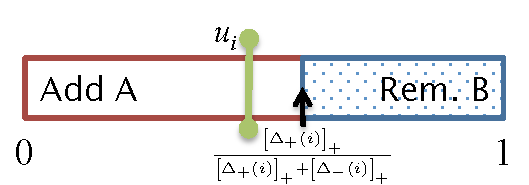
\includegraphics[width=130pt]{images/probvec_seq.pdf}
      \label{fig:probvecseq}
      \caption{\footnotesize\seqalg{}}
    \end{subfigure} &
    \begin{subfigure}[h]{0.30\textwidth}
      \centering
      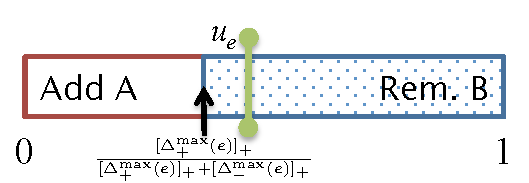
\includegraphics[width=130pt]{images/probvec_CF.pdf}
      \label{fig:probveccf}
      \caption{\footnotesize\hogwild{}}
    \end{subfigure} &
    \begin{subfigure}[h]{0.30\textwidth}
      \centering
      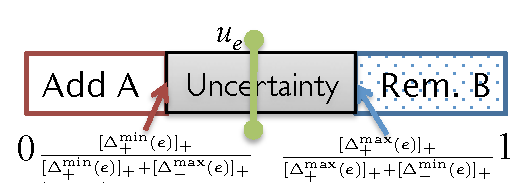
\includegraphics[width=130pt]{images/probvec_CC.pdf}
      \label{fig:probveccc}
      \caption{\footnotesize\occ{}}
    \end{subfigure}
  \end{tabular}
  \caption{\footnotesize Illustration of algorithms.
  \textbf{(a)} \seqalg{} computes a threshold based on the true values $\Delta_+$, $\Delta_-$, and chooses an action based by comparing a uniform random $u_i$ against the threshold.
  \textbf{(b)} \hogwild{} approximates the threshold based on stale $\hat{A}$, $\hat{B}$, possibly choosing the wrong action.
  \textbf{(c)} \occ{} computes two thresholds based on the bounds on $A$, $B$, which defines an uncertainty region where it is not possible to choose the correct action locally.  If the random value $u_e$ falls inside the uncertainty interval than the transaction FAILS and must be recomputed serially by the server otherwise the transaction holds under all possible global states. % at the time the transaction will be processed.
  }
\end{figure}


\section{Coordination Free Double Greedy Algorithm \label{sec:alghogwild}}
The coordination-free approach attempts to reduce the need to coordinate guarantees and logical ordering.
This is achieved by operating on potentially stale states -- the guarantee reduces to requiring $\mathfrak{g}_e$ be a stale version of $\mathfrak{S}$, and logical ordering is implicitly defined by the time of commit.
In using these weak guarantees, \hogwild{} is overly optimistically assuming that concurrent transactions are independent, which could potentially lead to erroneous decisions.
% \xinghao{An interesting take on hogwild -- hogwild is not serially equivalent to the sequential algorithm, but it is serially equivalent to an approximate algorithm that operates on stale states.
% Thus, to understand hogwild, we analyze the approximate algorithm.
% The concept of CC buys us two things: firstly, to extend sequential algorithms into parallel ones; secondly, to project a parallel algorithm into a sequential algorithm, which aids our understanding and analysis.}

\algref{alg:hogwild} is the coordination free parallel double greedy algorithm.\footnote{We present only the parallelized probabilistic versions of \cite{buchbinder2012}. Both parallel algorithms can be easily extended to the deterministic version of \cite{buchbinder2012}; \hogwild{} can also be extended to the multilinear version of \cite{buchbinder2012}.}
\hogwild{} closely resembles the serial \seqalg{}, but the elements $e \in V$ are no longer processed in a fixed order.  Thus, the sets $A, B$ are replaced by potentially stale ``bounds'' $\hat{A}, \hat{B}$, where $\hat{A}$ is a subset of the ``true'' $A$ and $\hat{B}$ is a superset of the ``actual'' $B$ on each iteration.
These bounding sets allow us to compute bounds $\Delta_{+}^{\max}, \Delta_{-}^{\max}$ which approximate $\Delta_{+}, \Delta_{-}$ from the serial algorithm.
We now formalize this idea.

We order the elements $e \in V$ according to the commit time, i.e. when \algref{alg:hogwild} line \ref{alg:hogwild:time} is executed.
Let $\iota(e)$ be the position of $e$ in this total ordering on elements.
This ordering allows us to define monotonically non-decreasing sets $A^i = \{e' : e' \in A, \iota(e') < i\}$, and monotonically non-increasing sets $B^i = A^i \cup \{e': \iota(e') \geq i\}$.
These ``true'' sets $A^i, B^i$ provide a serialization against which we can compare \hogwild{}; in this serialization, \algref{alg:submax} computes:
$\Delta_{+}       (e) = F(A^{\iota(e)-1}\cup i) - F(A^{\iota(e)-1})$
and
$\Delta_{-}       (e) = F(B^{\iota(e)-1}\backslash e) - F(B^{\iota(e)-1})$.
% \begin{align*}
%   \Delta_{+}       (e) &= F(A^{\iota(e)-1}\cup i) - F(A^{\iota(e)-1}),
% & \Delta_{-}       (e) &= F(B^{\iota(e)-1}\backslash e) - F(B^{\iota(e)-1}) \, .
% \end{align*}
On the other hand, \hogwild{} uses stale versions\footnote{
  For clarity, we present the algorithm as creating a copy of $\hat{A}$, $\hat{B}$, $\tilde{A}$, and $\tilde{B}$ for each element. In practice, it is more efficient to update and access them in shared memory. Nevertheless, our theorems hold for both settings.
  \label{fn:copyvsshared}
}
$\hat{A}_e$, $\hat{B}_e$:
\algref{alg:hogwild} computes
$\Delta_{+}^{\max}(e) = F(\hat{A}_e\cup e) - F(\hat{A}_e)$
and
$\Delta_{-}^{\max}(e) = F(\hat{B}_e\backslash e) - F(\hat{B}_e)$.
% \begin{align*}
%   \Delta_{+}^{\max}(e) &= F(\hat{A}_e\cup e) - F(\hat{A}_e),
% & \Delta_{-}^{\max}(e) &= F(\hat{B}_e\backslash e) - F(\hat{B}_e) \, .
% \end{align*}

The next lemma shows that $\hat{A}_e, \hat{B}_e$ are bounding sets for the serialization's sets $A^{\iota(e)-1}, B^{\iota(e)-1}$.
Intuitively, the bounds hold because $\hat{A}_e$, $\hat{B}_e$ are stale versions of $A^{\iota(e)-1}$, $B^{\iota(e)-1}$, which are monotonically non-decreasing and non-increasing sets.
Full details of proof are given in Appendix \ref{app:algoproof}.

\begin{restatable}{lem}{lemhogsetbound}\label{lem:hog:set_bound}
In \hogwild{}, for any $e\in V$, $\hat{A}_e \subseteq A^{\iota(e)-1}$, and $\hat{B}_e \supseteq B^{\iota(e)-1}$.
\end{restatable}

\begin{cor}\label{cor:hog:delta_bound}
Submodularity of $F$ implies for \hogwild{}
$\Delta_{+}(e) \leq \Delta_{+}^{\max}(e)$, and
$\Delta_{-}(e) \leq \Delta_{-}^{\max}(e)$.
\end{cor}

The error in \hogwild{} depends on the tightness of the bounds in \corref{cor:hog:delta_bound}.
We analyze this in \secref{sec:analysis:hogwild}.

% For some functions $F$, we can maintain sketches or statistics to aid the computation of $\Delta_+^{\max}$, $\Delta_-^{\max}$, and still obtain the bounds given in Corollary \ref{cor:hog:delta_bound}.
% In Appendix \ref{sec:sepsum}, we consider functions of separable sums, which are useful for applications such as document summarization \cite{lin11}.
%we consider functions of the form
%$F(X) = \sum_{l=1}^L g\left(\sum_{i\in X\cup S_l} w_l(i)\right) - \lambda\sum_{i\in X} v(i)$,
%where $S_l \subseteq V$ are (possibly overlapping) groups of elements in the ground set, $g$ is a non-decreasing concave scalar function, and $w_l(i)$ and $v(i)$ are non-negative scalar weights.










\section{Concurrency Control for Double Greedy Algorithm \label{sec:algocc}}
% \xinghao{Provide more intuition for what \occ{} is doing.}

\occ{}, the `concurrency-control double greedy' algorithm, is presented in \algref{alg:occ}, and closely follows the meta-algorithm of \algref{alg:generalparallel} and \algref{alg:generalparallel:commit}.
Unlike in \hogwild{}, the concurrency control mechanisms of \occ{} ensures that when concurrent transactions are serialized when they not indpendent.

Serializability is achieved by maintaining sets $\hat{A}$, $\tilde{A}$, $\hat{B}$, $\tilde{B}$, which serve as upper and lower bounds on $A$ and $B$ at commit time.
Each thread can determine locally if a decision to include / exclude an element can be taken safely.
Otherwise, the proposal is deferred to the commit process (\algref{alg:occcommit}) which waits until it is certain about $A$, $B$ before proceeding.

The commit order is given by $\iota(e)$, which is the value of $\iota$ at line \ref{alg:occ:time} of \algref{alg:occ}.
We define $A^{\iota(e)-1}$, $B^{\iota(e)-1}$ as before with \hogwild{}.
Additionally, let $\hat{A}_e$, $\hat{B}_e$, $\tilde{A}_e$, and $\tilde{B}_e$ be the sets that are returned by \algref{alg:occsnapshot}\footnoteref{fn:copyvsshared}.
Indeed, these sets are guaranteed to be bounds on $A^{\iota(e)-1}$, $B^{\iota(e)-1}$:

\begin{restatable}{lem}{lemoccsetbound}\label{lem:occ:set_bound}
In \occ{}, $\forall e\in V$,
$\hat{A}_e \subseteq A^{\iota(e)-1} \subseteq \tilde{A}_e \backslash e$, and $\hat{B}_e \supseteq B^{\iota(e)-1} \supseteq \tilde{B}_e \cup e$.
\end{restatable}
Intuitively, these bounds are maintained by recording potential effects of concurrent transactions in $\tilde{A}$, $\tilde{B}$, and only recording the actual effects in $\hat{A}$, $\hat{B}$;
we leave the full proof to Appendix \ref{app:algoproof}.
Furthermore, since later transactions are blocked, we have $\hat{A} = A^{\iota(e)-1}$ and $\hat{B} = B^{\iota(e)-1}$ at commit.

\begin{restatable}{lem}{lemoccdefer}\label{lem:occ:defer}
In \occ{}, during the commit process for deferred element $e$, we have $\hat{A} = A^{\iota(e)-1}$ and $\hat{B} = B^{\iota(e)-1}$.
\end{restatable}

% \algref{alg:occ} computes
% \begin{align*}
%   \Delta_+^{\min}(e) &= F(\tilde{A}_e) - F(\tilde{A}_e \backslash e),
% & \Delta_+^{\max}(e) &= F(\hat{A}_e \cup e) - F(\hat{A})\\
%   \Delta_-^{\min}(e) &= F(\tilde{B}_e) - F(\tilde{B}_e \cup e),
% & \Delta_-^{\max}(e) &= F(\hat{B}_e \backslash e) - F(\hat{B}).
% \end{align*}

\begin{cor}\label{cor:occ:delta_bound} Submodularity of $F$ implies that the $\Delta$'s computed by \occ{} satisfy: $\Delta_+^{\min}(e) \leq \Delta_+(e) = \Delta_+^{\text{exact}}(e) \leq \Delta_+^{\max}(e)$, and $\Delta_-^{\min}(e) \leq \Delta_-(e) = \Delta_+^{\text{exact}}(e) \leq \Delta_-^{\max}(e)$.
\end{cor}

% Like \hogwild{}, \occ{} can maintain statistics / sketches when dealing with functions of the form $F(X) = \sum_{l=1}^L g\left(\sum_{i\in X\cup S_l} w_l(i)\right) - \lambda\sum_{i\in X} v(i)$.
% We leave this discussion to Appendix \ref{sec:sepsum}.















\section{Analysis of Algorithms \label{sec:analysis}}

% \xinghao{What is the purpose of this section?
% We want to say that we have a choice between a slower but serially equivalent algorithm and a faster algorithm which is not serially equivalent.
% Nevertheless, the slower algorithm is not too slow, and the approximation guarantee of the algorithm that is not serially equivalent is not too weak.}

Our two algorithms appear to be diametrically opposed in their parallelization strategies.
However, we show that \hogwild{} emphasizes speed but nevertheless suffers a bounded loss in its approximation.
On the other hand, \occ{} is a scalable algorithm that guarantees the tight 1/2 approximation.


\subsection{Approximation of \hogwild{} double greedy \label{sec:analysis:hogwild}}
% Let $F$ be submodular and non-negative.
% We assume for each $e$, the random variable $\rho_e := \max\{\Delta_+^{\max}(e) - \Delta_+(e), \Delta_-^{\max}(e) - \Delta_-(e)\}$ is bounded.
% This is trivially possible since
% \begin{align*}
% \rho_e
% &&\leq&&& \max_{S,T\subseteq V} \{[F(S\cup e) - F(S)] - [F(S \cup T \cup e) - F(S \cup T)]\}
% &\leq&& F(e)\kappa_F
% \end{align*}
% where $\kappa_F$ is the total curvature of $F$.
% % Summing over $e$ then gives us $\sum_e \rho_e \leq \kappa_F\sum_e F(e)$.

\begin{restatable}{thm}{thmrandomapprox}\label{thm:randomapprox} Let $F$ be a non-negative (monotone or non-monotone) submodular function.
\hogwild{} solves the unconstrained problem $\max_{A\subset V} F(A)$ with approximation
$
E[F(A_{\hogwildshort{}})] \geq \frac{1}{2}F^* - \frac{1}{4}\sum_{i=1}^n E[\rho_i]$,
where $A_{\hogwildshort{}}$ is the output of the algorithm, $F^*$ is the optimal value, and $\rho_i = \max\{\Delta_+^{\max}(e) - \Delta_+(e), \Delta_-^{\max}(e) - \Delta_-(e)\}$.
\end{restatable}

The proof of \thmref{thm:randomapprox} follows the structure in \cite{buchbinder2012}. We present the details in Appendix \ref{app:proofhogwild}.



\textbf{Example: max graph cut.}
Assuming bounded delay of $\tau$ and edges with unit weight, we can bound $\sum_i E[\rho_i] \leq 2\tau\frac{\text{\#edges}}{2N}$
The approximation of \hogwild{} is then $E[F(A^n)] \geq = \frac{1}{2} F(OPT) - \tau\frac{\#\text{edges}}{2N}$.
In sparse graphs, \hogwild{} is off by a small additional term, which albeit grows linearly in $\tau$.
In a complete graph, $F^* = \frac{1}{2}\#\text{edges}$, so $E[F(A^n)] \geq F^*\left(\frac{1}{2} - \frac{\tau}{N}\right)$, which makes it possible to scale $\tau$ linearly with $N$ while retaining the same approximation factor.


\textbf{Example: set cover.}
Consider the simple set cover function,
$F(A) = \sum_{l=1}^L \min(1,|A\cap S_l|) - \lambda|A| = |\{l: A\cap S_l \neq\emptyset\}| - \lambda|A|$,
with $0 < \lambda \leq 1$.
We assume that there is some bounded delay $\tau$.
Suppose also the $S_l$'s form a partition, so each element $e$ belongs to exactly one set.
Then, $\sum_e E[\rho_e] \geq \tau + L(1-\lambda^\tau)$, which is linear in $\tau$ but independent of $N$.



\subsection{Correctness of \occ{}}
\begin{restatable}{thm}{thmoccserializable} \occ{} is serializable.
\end{restatable}
% We prove the serializability by induction on the commit order of elements.
It suffices to show that \occ{} takes the same decision as \seqalg{} for each element -- locally if it is safe to do so, and otherwise deferring to the server.
Full details of the proof are given in Appendix \ref{app:occserializable}.
As an immediate consequence, theoretical properties of \seqalg{} are preserved by \occ{}, including the approximation guarantees:

\begin{thm} Let $F$ be a non-negative (monotone or non-monotone) submodular function.
\occ{} solves the unconstrained problem $\max_{A\subset V} F(A)$ with approximation
$E[F(A_{\occshort{}})] \geq \frac{1}{2}F^*$,
where $A_{\occshort{}}$ is the output of the algorithm, and $F^*$ is the optimal value.
\end{thm}




\subsection{Scalability of \occ{}}
Whenever an element deferred for computation the server, it needs to wait for all earlier elements to be processed, and the server is blocked from committing all later elements.
Each deferment effectively constitutes a barrier to the parallel processing.
Hence, the scalability of \occ{} is dependent on the number of deferments.
Nevertheless, we show for a couple of example problems that the number of deferments can be bounded.
Full details of the bounds are given in Appendix \ref{app:proofocc}.

\textbf{Example: max graph cut.}
Assume that there is a bounded delay $\tau$.
The expected \emph{fraction} of deferred elements is upper bounded by $\tau \frac{2\#edges}{N^2}$.

\textbf{Example: set cover.}
Assuming a bounded delay $\tau$ and non-overlapping sets $S_l$'s, the expected \emph{number} of deferred elements is upper bounded by $2\tau$.

















\section{Evaluation \label{sec:evaluation}}

We implemented the parallel and sequential double greedy algorithms in Java / Scala.
Experiments were conducted on Amazon EC2 using one cc2.8xlarge machine, up to 16 threads, for 10 repetitions.

We measured the runtime and speedup (ratio of runtime on 1 thread to runtime on $p$ threads).
For \hogwild{}, we measured $F(A_{\hogwildshort})-F(A_{\seqalgshort})$, the difference between the objective value on the sets returned by \hogwild{} and \seqalg{}.
We verified the correctness of \occ{} by comparing the output of \occ{} with \seqalg{}.
We also the fraction of elements deferred by \occ{}.

%\begin{table}[h]
%\centering
%\begin{tabular}{|c|c|c|c|}\hline
%Graph & \# vertices & \# undirected edges & \# directed edges\\\hline\hline
%Google       &    875,713 &     3,852,985 &   4,563,235\\\hline
%BerkStan     &    685,230 &     6,649,470 &   7,600,595\\\hline
%Live Journal &  3,997,962 &    40,592,387 &  40,592,387\\\hline
%Orkut        &  3,072,441 &   117,181,608 & 117,181,608\\\hline
%Friendster   &  8,000,000 &   239,730,456 & 239,730,456\\\hline
%Friendster   & 10,000,000 &   625,279,786 & 625,279,786\\\hline
%Arabic-2005  & 22,744,080 & 1,107,806,146 & 631,153,669\\\hline
%UK-20005     & 39,459,925 & 1,566,054,250 & 921,345,078\\\hline
%\end{tabular}
%\end{table}
%\end{comment}

\begin{table}[h]
\centering\footnotesize
\begin{tabular}{|c|c|c|c|}\hline
Graph & \# vertices & \# edges & Description \\\hline\hline
Erdos-Renyi & 20,000,000 & $\approx 2 \times 10^6$ & Each edge is included with probability $5\times 10^{-6}$.\\\hline
\multirow{3}{*}{ZigZag}      & \multirow{3}{*}{25,000,000} &  \multirow{3}{*}{2,025,000,000} & Expander graph. The 81-regular zig-zag product \\
& & & between the Cayley graph on $\mathbb{Z}_{2500000}$ with generating \\
& & & set $\{\pm 1,\dots,\pm 5\}$, and the complete graph $K_{10}$.\\\hline
Friendster  & 10,000,000 &    625,279,786 & Subgraph of social network. \cite{snap}\\\hline
Arabic-2005 & 22,744,080 &    631,153,669 & 2005 crawl of Arabic web sites \cite{BoVWFI, BRSLLP, BCSU3}. \\\hline
UK-2005     & 39,459,925 &    921,345,078 & 2005 crawl of the .uk domain \cite{BoVWFI, BRSLLP, BCSU3}. \\\hline
IT-2004     & 41,291,594 &  1,135,718,909 & 2004 crawl of the .it domain \cite{BoVWFI, BRSLLP, BCSU3}. \\\hline
\end{tabular}
\caption{\footnotesize Synthetic and real graphs used in the evaluation of our parallel algorithms.}
\label{tab:graphstats}
\end{table}



We tested our parallel algorithms on the max graph cut and set cover problems with two synthetic graphs and three real datasets (Table \ref{tab:graphstats}).
% Graphs were pre-processed to remove self-loops.
We found that vertices were typically indexed such that vertices close to each another in the graph were also close in their indices.
To reduce this dependency, we randomly permuted the ordering of vertices.
% For the max graph cut problem, we removed directions on edges to obtain undirected graphs.
% The set cover problem is reduced to a vertex cover on the directed graph.


\begin{figure}[ht]
  \centering
  \begin{tabular}{cccc}
	  \begin{subfigure}[h]{0.30\textwidth}
	  	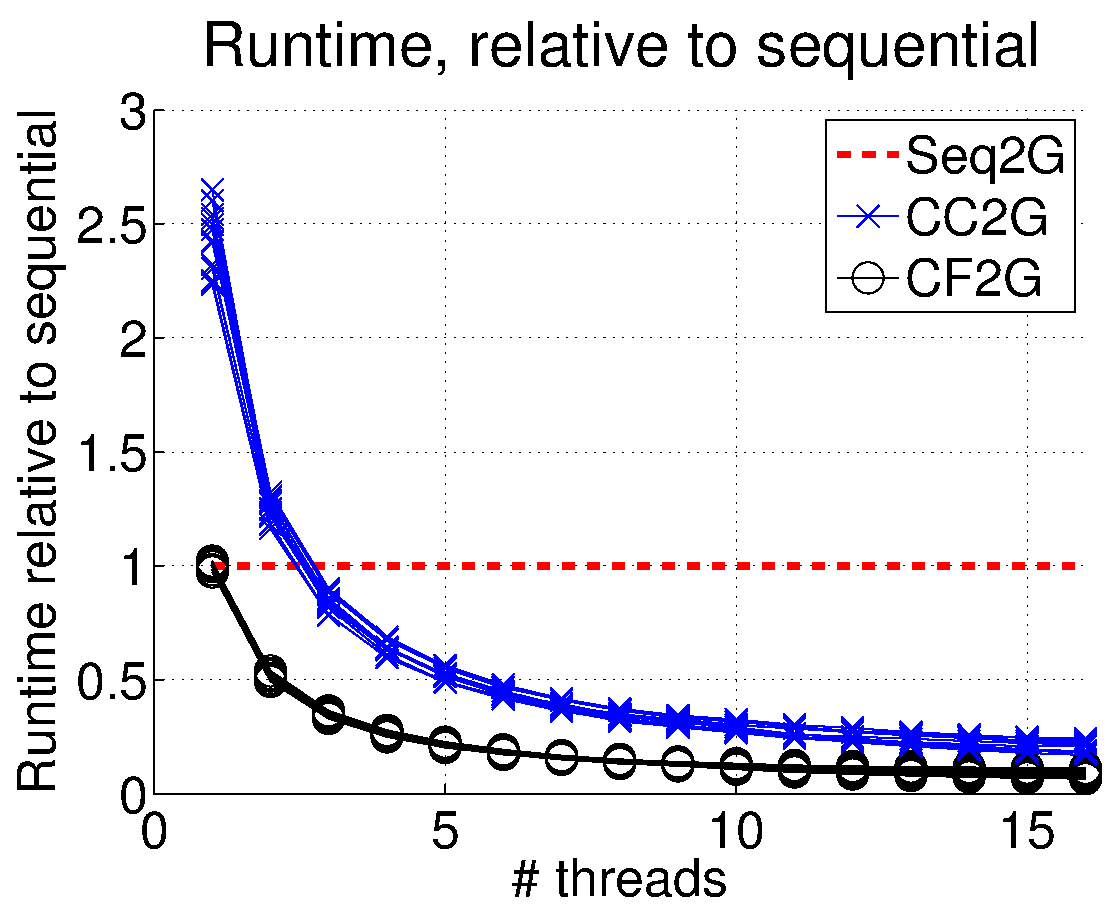
\includegraphics[width=130pt]{images/summary_relruntime.pdf}
			\caption{}
			\label{fig:relruntime}
	  \end{subfigure} &
	  \begin{subfigure}[h]{0.30\textwidth}
	  	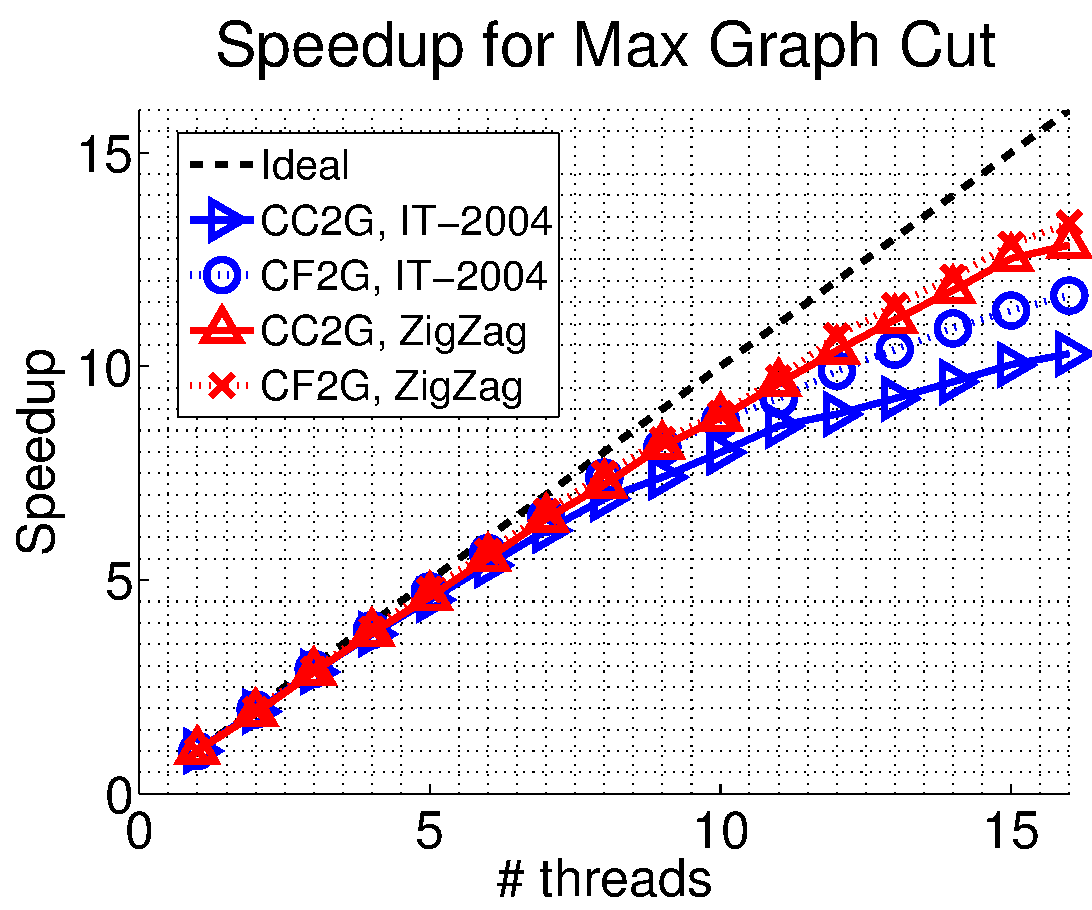
\includegraphics[width=130pt]{images/summary_speedup_maxgraphcut.pdf}
			\caption{}
			\label{fig:speedup_maxgraphcut}
	  \end{subfigure} &
	  \begin{subfigure}[h]{0.30\textwidth}
	  	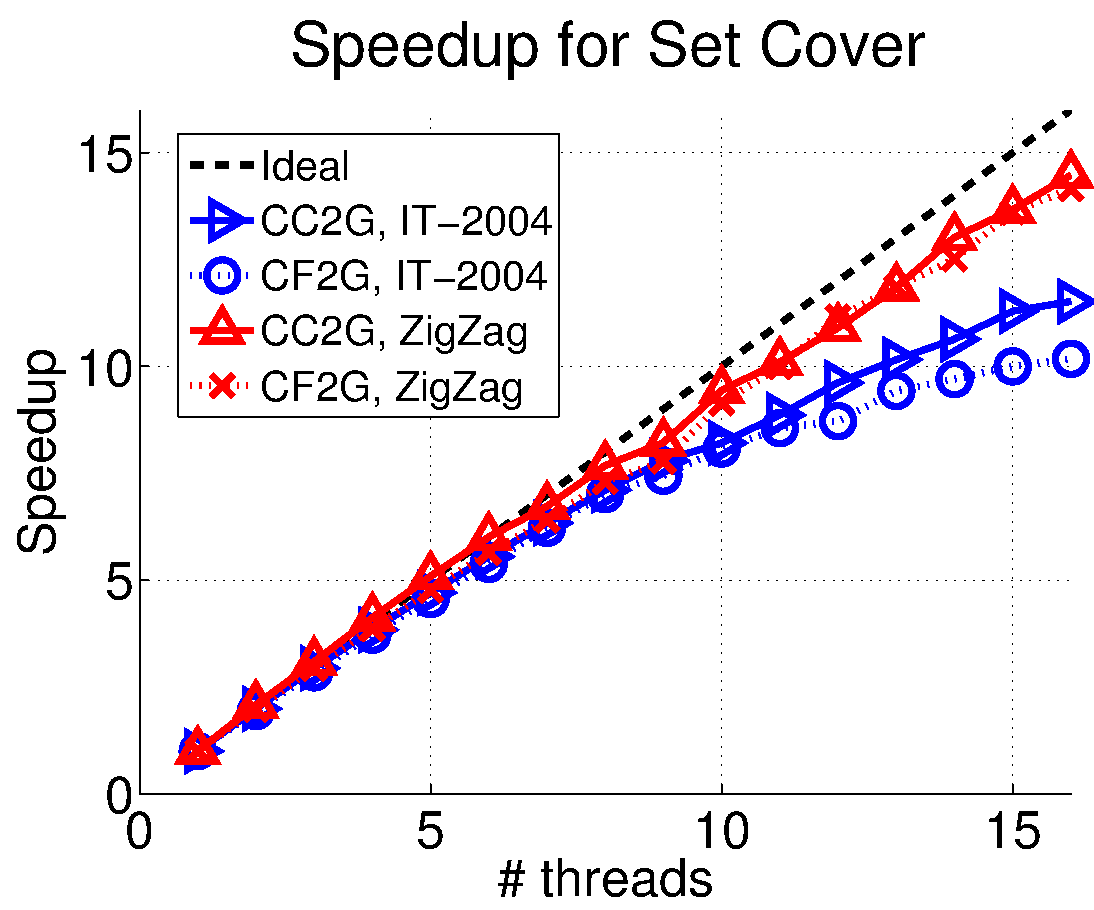
\includegraphics[width=130pt]{images/summary_speedup_setcover.pdf}
			\caption{}
			\label{fig:speedup_setcover}
	  \end{subfigure} \\
	  \begin{subfigure}[h]{0.30\textwidth}
	  	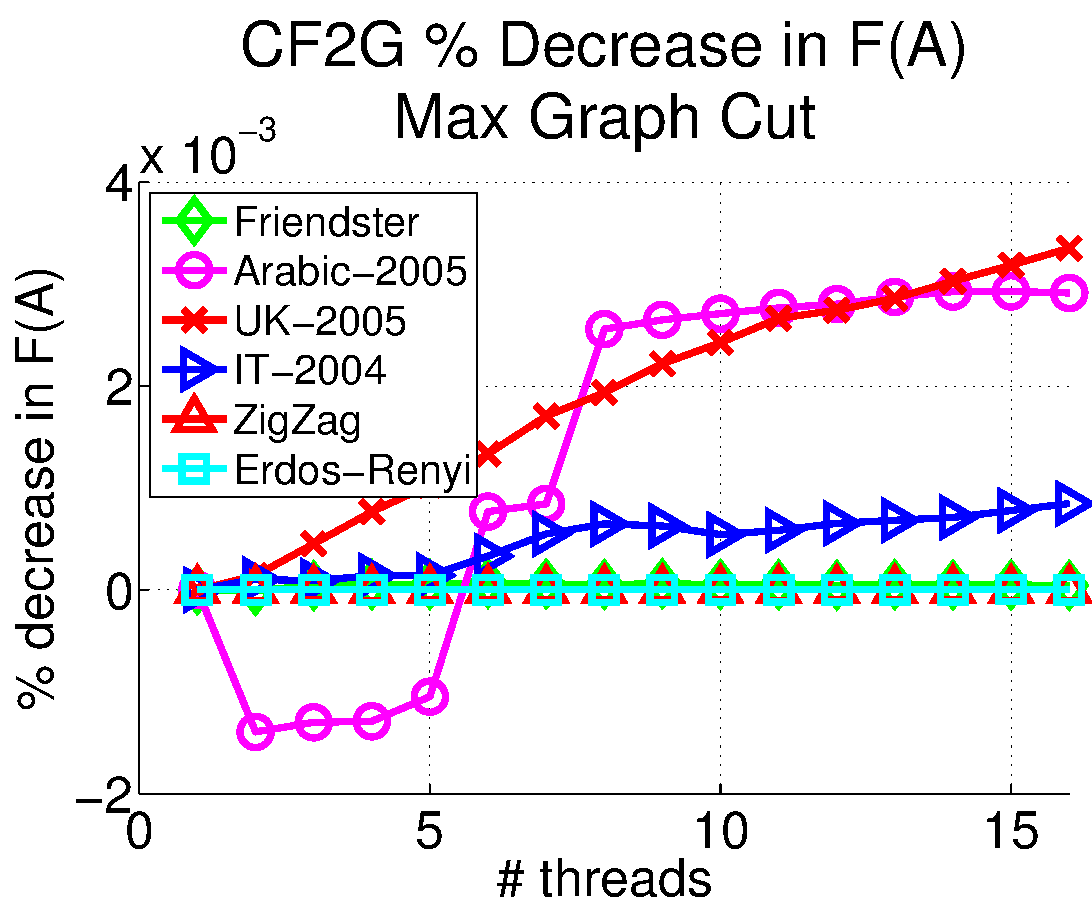
\includegraphics[width=130pt]{images/summary_diffFA_maxgraphcut.pdf}
			\caption{}
			\label{fig:difffa_maxgraphcut}
	  \end{subfigure} &
	  \begin{subfigure}[h]{0.30\textwidth}
	  	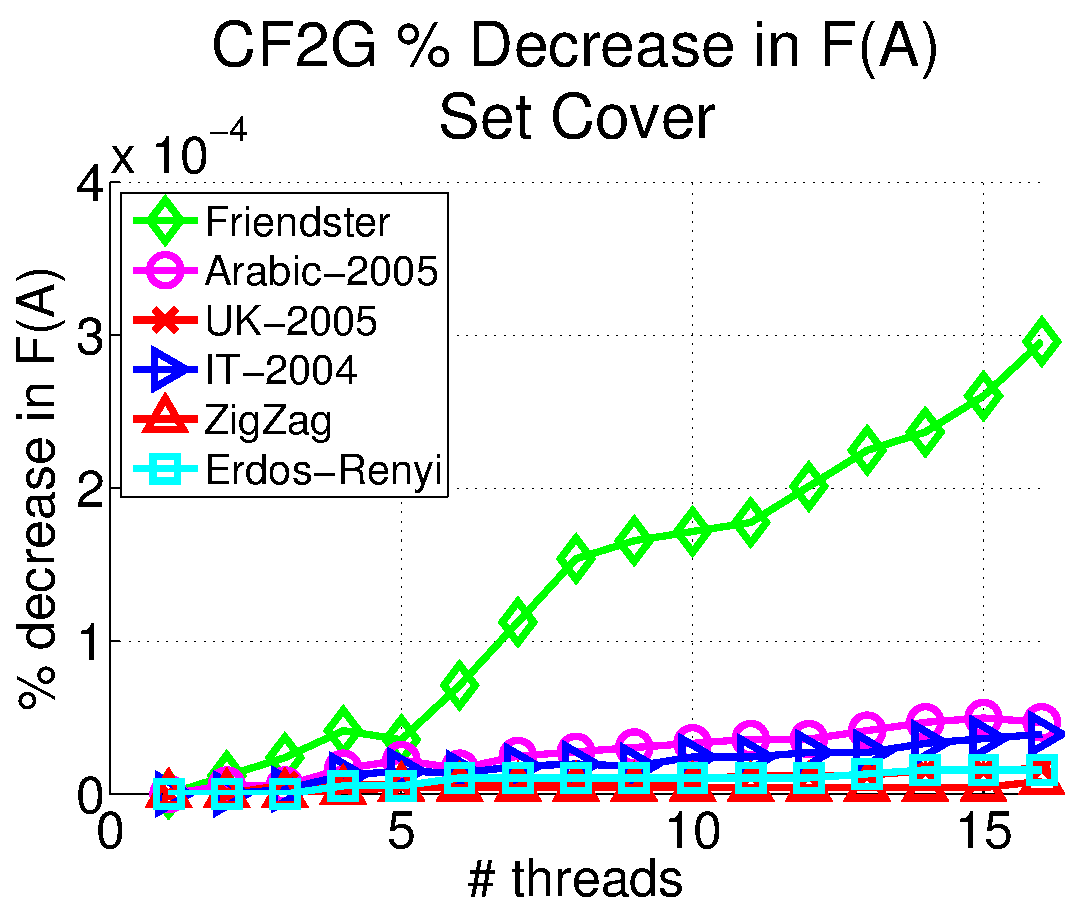
\includegraphics[width=130pt]{images/summary_diffFA_setcover.pdf}
			\caption{}
			\label{fig:difffa_setcover}
	  \end{subfigure} &
	  \begin{subfigure}[h]{0.30\textwidth}
	  	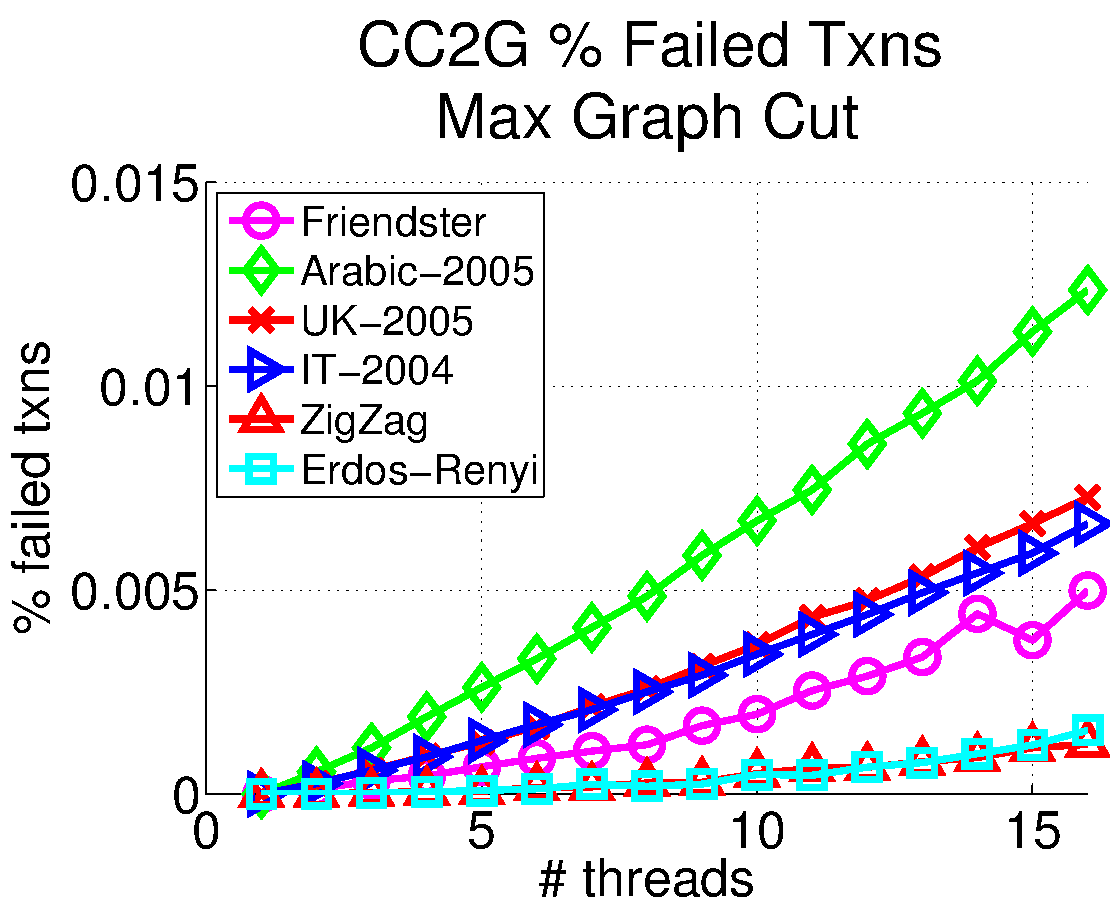
\includegraphics[width=130pt]{images/summary_validated_maxgraphcut.pdf}
			\caption{}
			\label{fig:validated_maxgraphcut}
	  \end{subfigure} \\
  \end{tabular}
  \caption{\footnotesize Experimental results.
  \figref{fig:relruntime} -- runtime of the parallel algorithms as a ratio to that of the sequential algorithm. Each curve shows the runtime of a parallel algorithm on a particular graph for a particular function $F$.
  \figref{fig:speedup_maxgraphcut}, \ref{fig:speedup_setcover} -- speedup (ratio of runtime on one thread to that on $p$ threads).
  \figref{fig:difffa_maxgraphcut}, \ref{fig:difffa_setcover} -- \% difference between objective values of \seqalg{} and \hogwild{}, i.e. $[F(A_{\hogwildshort{}}) / F(A_{\seqalgshort{}}) - 1] \times 100\%$.
  \figref{fig:validated_maxgraphcut} -- percentage of elements deferred by \occ{} on the max graph cut problem.
  }
\label{fig:results_quality}
\end{figure}


Due to space constraints, we only present part of our results in \figref{fig:results_quality}, deferring full results to Appendix \ref{app:exptresults}.
\textbf{Runtime, Speedup:} Both parallel algorithms are faster than the sequential algorithm with three or more threads, and show good speedup properties as more threads are added ($\sim$ 10x or more for all graphs and both functions).
\textbf{Objective value:} The objective value of \hogwild{} decreases with the number of threads, but differs from the sequential objective value by less than $0.01\%$.
\textbf{Deferments:} \occ{} defers more elements as threads are added, but less than 0.015\% are deferred with 16 threads, which has negligible effect on the runtime / speedup.

\subsection{Adversarial ordering}

To highlight the differences in approaches between the two parallel algorithms, we conducted experiments on a ring Cayley graph on $\mathbb{Z}_{10^6}$ with generating set $\{\pm 1,\dots, \pm 1000\}$.
The algorithms are presented with an adversarial ordering, without permutation, so vertices close in the ordering are adjacent to one another, and tend to be processed concurrently.
This causes \hogwild{} to make more mistakes, and \occ{} to defer more proposals.
% \xinghao{These experiments were conducted by using an atomic integer to select elements to process. We could instead use a partitioning scheme, which has 2 advantages. Firstly, there is less coordination -- for \hogwild{}, we essentially have no coordination.
% Secondly, when faced with an adversarial ordering, the partitioning scheme allows big jumps / re-orderings, which reduces the number of validations and \textit{increases} the objective value of both parallel algorithms.}
\footnote{
We point out by using a partitioning scheme, it is possible to avoid the problems caused by the adversarial ordering, and to improve scalability.
Nevertheless, we present results that do \emph{not} use the partitioning scheme, so as to better highlight the differences between the two parallel algorithms.
}
As \figref{fig:results_adversarial} shows, \occ{}  sacrifices speed to ensure serial equivalence, eventually deferring $>90\%$ of elements.
On the other hand, \hogwild{} focuses on speed, resulting in faster runtime, but delivering an objective value $F(A_{\hogwildshort{}})$ that is $20\%$ of $F(A_{\seqalgshort{}})$.
% For the set cover problem, we maintain statistics that are updated atomically by both algorithms.
% The adversarial ordering forces more concurrent atomic updates, and hence, \hogwild{} does not achieve good speedup.
% \footnote{We could have reduced coordination by computing $F$ directly, but doing so would result in longer runtimes.}

\begin{figure}[ht]
  \centering
  \begin{tabular}{cccc}
	  \begin{subfigure}[h]{0.30\textwidth}
	  	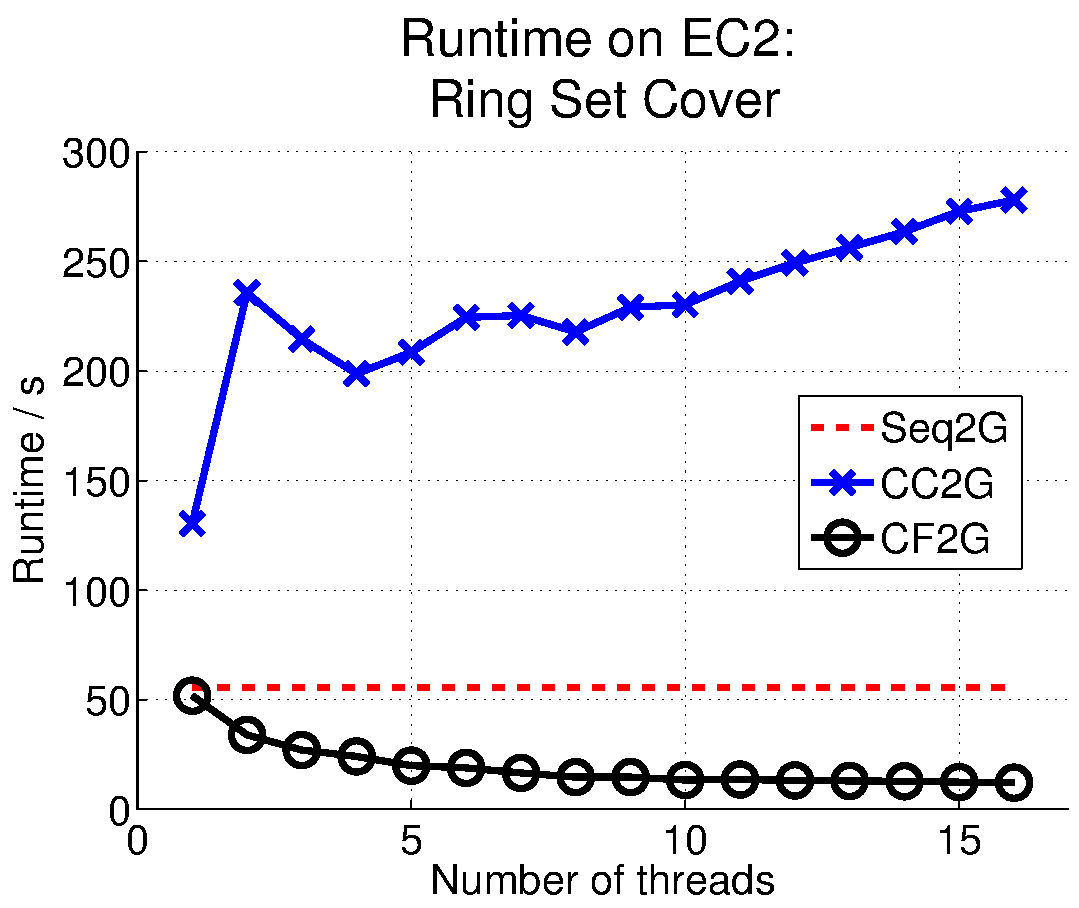
\includegraphics[width=130pt]{images/runtime_ring_setcover.pdf}
			\caption{}
			\label{fig:runtime_ring_setcover}
	  \end{subfigure} &
	  \begin{subfigure}[h]{0.30\textwidth}
	  	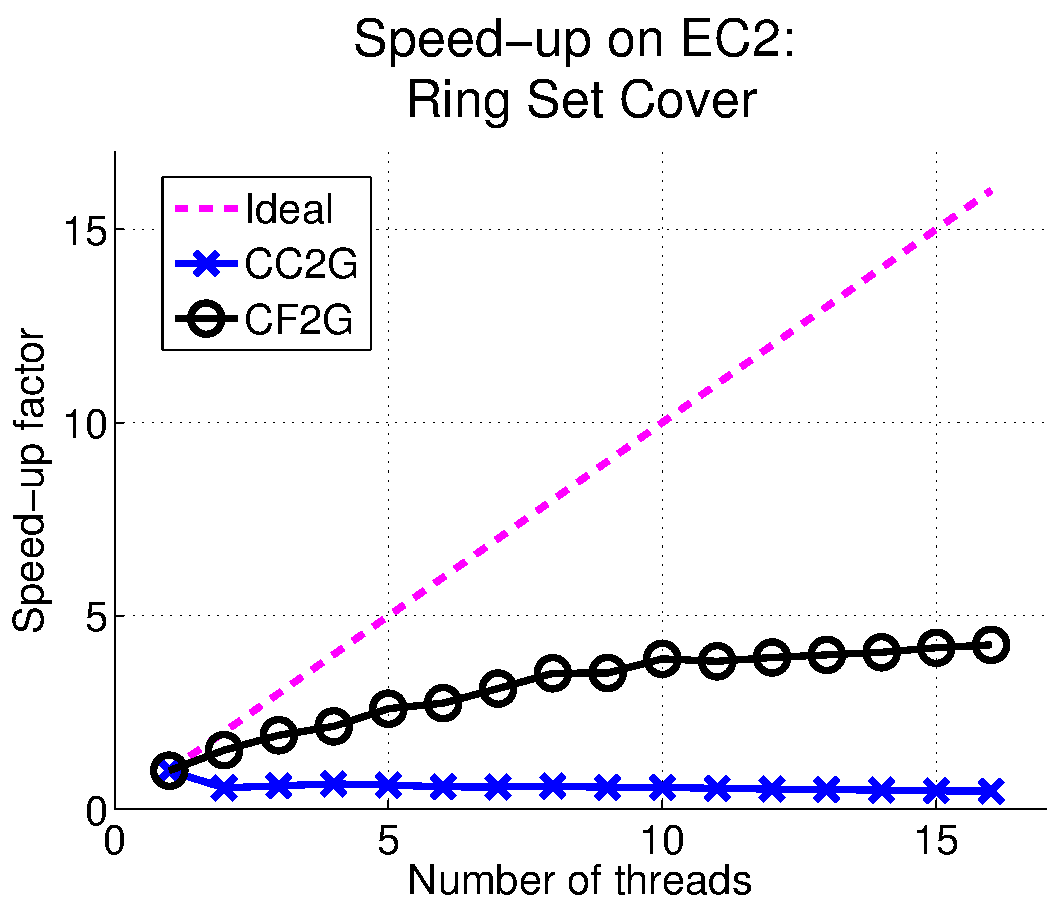
\includegraphics[width=130pt]{images/speedup_ring_setcover.pdf}
			\caption{}
			\label{fig:speedup_ring_setcover}
	  \end{subfigure} &
	  \begin{subfigure}[h]{0.30\textwidth}
	  	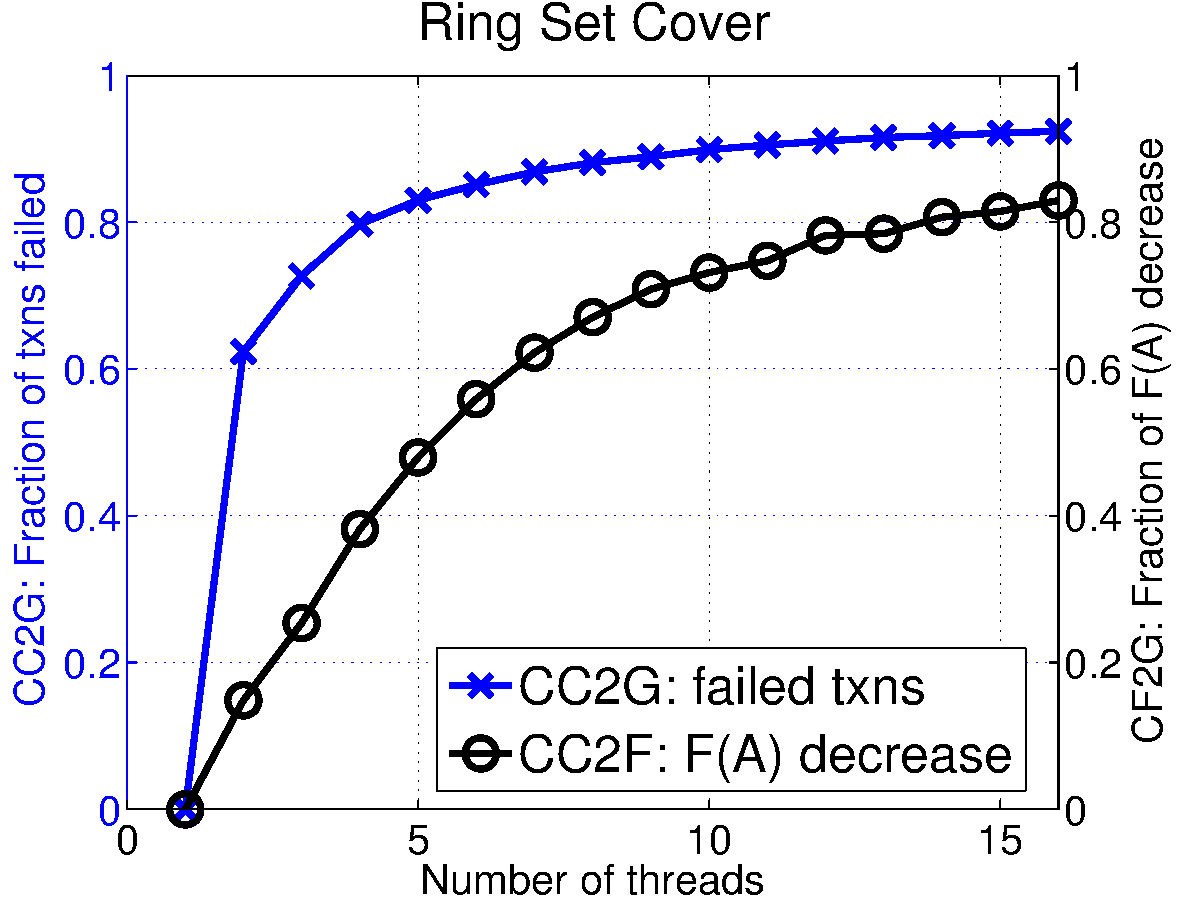
\includegraphics[width=130pt]{images/validateddiffFA_ring_setcover.pdf}
			\caption{}
			\label{fig:validateddiffFA_ring_setcover}
	  \end{subfigure} \\
  \end{tabular}
  \caption{\footnotesize Experimental results for ring graph on set cover problem.}
\label{fig:results_adversarial}
\end{figure}










\section{Related Work \label{sec:related}}
\textbf{Similar approach: }
Coordination-free solutions have been proposed for stochastic gradient descent \cite{Recht11} and collapsed Gibbs sampling \cite{Ahmed12}.
More generally, parameter servers \cite{li2013, ho2013} apply the \hogwildshort{} approach to larger classes of problems.
\cite{pan2013} applied concurrency control to parallelize some unsupervised learning algorithms.
\textbf{Similar problem: } \cite{Mirzasoleiman2013} explored distributed greedy submodular maximization, but only applied to monotone functions.






\section{Discussions \label{sec:discussions}}

We present two approaches to parallelizing the double greedy algorithm for unconstrained submodular maximization.
We quantify the weaker approximation guarantee of \hogwild{} and the additional coordination of \occ{}, allowing one to trade-off between performance and objective optimality.
Our evaluation on large scale data demonstrates the scalability and tradeoffs of the two approaches.

We believe there are a number of areas for future work.
One can imagine a system that allows a smooth interpolation between \hogwild{} and \occ{}.
While both \hogwild{} and \occ{} can be immediately implemented as distributed algorithms, higher communication costs and delays may pose additional challenges.
Finally, other problems such as constrained maximization of monotone / non-monotone functions could potentially be parallelized with the \hogwildshort{} and \occshort{} frameworks.

\newpage
{\footnotesize
%\subsection*{Acknowledgments}
%This research is supported in part by NSF CISE Expeditions award CCF-1139158 and DARPA XData Award FA8750-12-2-0331, and  gifts from Amazon Web Services, Google, SAP,  Blue Goji, Cisco, Clearstory Data, Cloudera, Ericsson, Facebook, General Electric, Hortonworks, Intel, Microsoft, NetApp, Oracle, Samsung, Splunk, VMware and Yahoo!.
%This material is also based upon work supported in part by the Office of
%Naval Research under contract/grant number N00014-11-1-0688.
%X. Pan's work is also supported in part by a DSO National Laboratories Postgraduate Scholarship.

% In the unusual situation where you want a paper to appear in the
% references without citing it in the main text, use \nocite
%\nocite{langley00}

\bibliographystyle{unsrtnat}
\bibliography{references_arxiv}
}

\newpage
\appendix



% \section{Parallel algorithms for separable sums}
\label{sec:sepsum}
\begin{figure}[H]
  \footnotesize
  \centering
  \begin{multicols}{2}
    \begin{minipage}{0.49\textwidth}
      \begin{algorithm}[H]
        \DontPrintSemicolon
        \caption{\hogwild{} for separable sums}
        \label{alg:hogwildsepsum}
        \lFor{$e\in V$}{$\hat{A}(e) = 0$}\;
        \lFor{$l = 1,\dots,L$}{$\hat\alpha_l = 0$, $\hat\beta_l = \sum_{e\in S_l}w_l(e)$}\;
        \ParForAll{$p \in \set{1, \ldots, P}$}{
          \While{$\exists$ element to process}{
            $e = $ next element to process\;
            $\Delta_+^{\max}(e) = -\lambda v(e) + \sum_{S_l\ni e} g(\hat\alpha_l + w_l(e)) - g(\hat\alpha_l)$\;
            $\Delta_-^{\max}(e) = +\lambda v(e) + \sum_{S_l\ni e} g(\hat\beta_l   - w_l(e)) - g(\hat\beta_l)$\;
            Draw $u_e\sim Unif(0,1)$\;
            \If {$u_e<\frac{[\Delta_{+}^{\max}(e)]_+}{[\Delta_{+}^{\min}(e)]_+ + [\Delta_{-}^{\max}(e)]_+}$}{
              $\hat{A}(e) \leftarrow 1$\;
              \lFor{$l: e \in S_l$}{
                $\hat\alpha_l \leftarrow \hat\alpha_l + w_l(e)$
              }
            }\lElse{
              \lFor{$l: e \in S_l$}{
                $\hat\beta_l \leftarrow \hat\beta_l - w_l(e)$
              }
            }
          }
        }
      \end{algorithm}
      \begin{algorithm}[H]
        \DontPrintSemicolon
        \caption{\occ{} validate for separable sums}
        \label{alg:occsepsumvalidate}
        \WaitUntil $\forall j < i$, processed$(j) = true$\;
        $\Delta_+^{\text{exact}}(e) = -\lambda v(e) + \sum_{S_l\ni e} g(\hat\alpha_l + w_l(e)) - g(\hat\alpha_l)$\;
        $\Delta_-^{\text{exact}}(e) = +\lambda v(e) + \sum_{S_l\ni e} g(\hat\beta_l   - w_l(e)) - g(\hat\beta_l)$\;
        \lIf {$u_e < \frac{[\Delta_+^{\text{exact}}(e)]_+}{[\Delta_+^{\text{exact}}(e)]_+ + [\Delta_-^{\text{exact}}(e)]_+}$}{
          result$(i) \leftarrow 1$\;
        }\lElse{
          result$(i) \leftarrow -1$\;
        }
      \end{algorithm}

    \end{minipage}

    \begin{minipage}{0.49\textwidth}
      \begin{algorithm}[H]
        \DontPrintSemicolon
        \caption{\occ{} for separable sums}
        \label{alg:occsepsum}
        \lFor{$e\in V$}{$\hat{A}(e) = \tilde{A}(e) = 0$, $\hat{B}(e) = \tilde{B}(e) = 1$}\;
        \For{$l = 1,\dots,L$}{
          $\hat\alpha_l = \tilde\alpha_l = 0$\;
          $\hat\beta_l = \tilde\beta_l = \sum_{e\in S_l}w_l(e)$\;
        }
        \lFor{$i = 1,\dots,|V|$}{result$(i) = 0$}\;
        \lFor{$i = 1,\dots,|V|$}{processed$(i) = false$}\;
        $\iota = 0$\;
        \ParForAll{$p \in \set{1, \ldots, P}$}{
          \While{$\exists$ element to process}{
            $e = $ next element to process\;
            $\tilde{A}(e) \leftarrow 1$\;
            $\tilde{B}(e) \leftarrow 0$\;
            \For{$l: e \in S_l$}{
              $\tilde\alpha_l \leftarrow \tilde\alpha_l + w_l(e)$\;
              $\tilde\beta_l  \leftarrow \tilde\beta_l  - w_l(e)$\;
            }
            $i = \iota$; $\iota \leftarrow \iota + 1$\;
            $\Delta_+^{\min}(e) = -\lambda v(e) + \sum_{S_l\ni e} g(\tilde\alpha_l) - g(\tilde\alpha_l - w_l(e))$\;
            $\Delta_+^{\max}(e) = -\lambda v(e) + \sum_{S_l\ni e} g(\hat\alpha_l + w_l(e)) - g(\hat\alpha_l)$\;
            $\Delta_-^{\min}(e) = +\lambda v(e) + \sum_{S_l\ni e} g(\tilde\beta_l) - g(\tilde\beta_l + w_l(e))$\;
            $\Delta_-^{\max}(e) = +\lambda v(e) + \sum_{S_l\ni e} g(\hat\beta_l   - w_l(e)) - g(\hat\beta_l)$\;
            Draw $u_e \sim Unif(0,1)$\;
            \If {$u_e < \frac{[\Delta_+^{\min}(e)]_+}{[\Delta_+^{\min}(e)]_+ + [\Delta_-^{\max}(e)]_+}$}{
              result$(i) \leftarrow 1$\;
            }\ElseIf {$u_e > \frac{[\Delta_+^{\max}(e)]_+}{[\Delta_+^{\max}(e)]_+ + [\Delta_-^{\min}(e)]_+}$}{
              result$(i) \leftarrow -1$\;
            }
            \WaitUntil $\forall j<i$, result$(j) \neq 0$\;
            \lIf {result$(i) = 0$}{validate($p$, $e$, $i$)}\;
            \If {result$(i) = 1$}{
              $\hat{A}(e)   \leftarrow 1$\;
              $\tilde{B}(e) \leftarrow 1$\;
              \For{$l: e \in S_l$}{
                $\hat\alpha_l   \leftarrow \hat\alpha_l   + w_l(e)$\;
                $\tilde\beta_l  \leftarrow \tilde\beta_l  + w_l(e)$\;
              }
            }\Else{
              $\tilde{A}(e) \leftarrow 0$\;
              $\hat{B}(e)   \leftarrow 0$\;
              \For{$l: e \in S_l$}{
                $\tilde\alpha_l \leftarrow \tilde\alpha_l - w_l(e)$\;
                $\hat\beta_l    \leftarrow \hat\beta_l    - w_l(e)$\;
              }
            }
            processed$(i) = true$\;
          }
        }
      \end{algorithm}
    \end{minipage}
  \end{multicols}
\end{figure}

For some functions $F$, we can maintain sketches / statistics to aid the computation of $\Delta_+^{\max}$, $\Delta_-^{\max}$, $\Delta_+^{\min}$, $\Delta_-^{\min}$.
In particular, we consider functions of the form
$F(X) = \sum_{l=1}^L g\left(\sum_{i\in X\cup S_l} w_l(i)\right) - \lambda\sum_{i\in X} v(i)$,
where $S_l \subseteq V$ are (possibly overlapping) groups of elements in the ground set, $g$ is a non-decreasing concave scalar function, and $w_l(i)$ and $v(i)$ are non-negative scalar weights.
It is easy to see that
$
F(X \cup e) - F(X) = \sum_{l: e\in S_l} \left[g\left(w_l(e) + \sum_{i\in X\cup S_l} w_l(i)\right) - g\left(\sum_{i\in X\cup S_l} w_l(i)\right)\right] - \lambda v(e)$.
Define
%  $\hat\alpha_l              = \sum_{j\in \hat{A}\cup S_l} w_l(j)$,
% $\hat\alpha_{l,e}          = \sum_{j\in \hat{A}_e\cup S_l} w_l(j)$,
% $\alpha_l^{\iota(e)-1} = \sum_{j\in A^{\iota(e)-1}\cup S_l} w_l(j)$.
%
%  $\hat\beta_l              = \sum_{j\in \hat{B}\cup S_l} w_l(j)$,
% $\hat\beta_{l,e}          = \sum_{j\in \hat{B}_e\cup S_l} w_l(j)$,
% $\beta_l^{\iota(e)-1} = \sum_{j\in B^{\iota(e)-1}\cup S_l} w_l(j)$.
%
\begin{align*}
  \hat\alpha_l              &= \sum_{j\in \hat{A}\cup S_l} w_l(j),
& \hat\alpha_{l,e}          &= \sum_{j\in \hat{A}_e\cup S_l} w_l(j),
& \alpha_l^{\iota(e)-1} &= \sum_{j\in A^{\iota(e)-1}\cup S_l} w_l(j).\\
  \hat\beta_l              &= \sum_{j\in \hat{B}\cup S_l} w_l(j),
& \hat\beta_{l,e}          &= \sum_{j\in \hat{B}_e\cup S_l} w_l(j),
& \beta_l^{\iota(e)-1} &= \sum_{j\in B^{\iota(e)-1}\cup S_l} w_l(j).
\end{align*}


\subsection{\hogwild{} for separable sums $F$}
Algorithm \ref{alg:hogwildsepsum} updates $\hat\alpha_l$ and $\hat\beta_l$, and computes $\Delta_+^{\max}(e)$ and $\Delta_-^{\max}(e)$ using $\hat\alpha_{l,e}$ and $\hat\beta_{l,e}$.
Following arguments analogous to that of Lemma \ref{lem:hog:set_bound}, we can show:

\begin{lem} For each $l$ and $e\in V$, $\hat\alpha_{l,e} \leq \alpha_l^{\iota(e)-1}$ and $\hat\beta_{l,e} \geq \beta_l^{\iota(e)-1}$.
\end{lem}

\begin{cor} Concavity of $g$ implies that $\Delta$'s computed by Algorithm \ref{alg:hogwildsepsum} satisfy
\begin{align*}
\Delta_+^{\max}(e)
&&\geq&& \sum_{S_l\ni e} \left[g(\alpha_l^{\iota(e)-1} + w_l(e)) - g(\alpha_l^{\iota(e)-1})\right] - \lambda v(e)
&&=&& \Delta_+(e),\\
\Delta_-^{\max}(e)
&&\geq&& \sum_{S_l\ni e} \left[g(\beta_l^{\iota(e)-1} - w_l(e)) - g(\beta_l^{\iota(e)-1})\right] + \lambda v(e)
&&=&& \Delta_-(e),
\end{align*}
\end{cor}

\subsection{\occ{} for separable sums $F$}
Analogous to the \hogwild{} algorithm, we maintain $\hat\alpha_l$, $\hat\beta_l$ and additionally $\tilde\alpha_l = \sum_{j\in \tilde{A}\cup S_l} w_l(j)$ and $\tilde\beta_l = \sum_{j \in \tilde{B}\cup S_l} w_l(j)$.
Following the arguments of Lemma \ref{lem:occ:set_bound} and Corollary \ref{cor:occ:delta_bound}, we can show the following.
\begin{lem} $\hat\alpha_{l,e} \leq \alpha^{\iota(e)-1} \leq \tilde\alpha_{l,e} - w_l(e)$ and $\hat\beta_{l,e} \geq \beta^{\iota(e)-1} \geq \tilde\beta_{l,e} + w_l(e)$
\end{lem}

\begin{cor} Concavity of $g$ implies that the $\Delta$'s computed by Algorithm \ref{alg:occsepsum} satisfy:
\begin{align*}
\Delta_+^{\max}(e)
&= - \lambda v(e) + \sum_{S_l \ni e} \left[g(\hat\alpha_{l,e} + w_l(e)) - g(\hat\alpha_{l,e})\right]\\
&\geq - \lambda v(e) + \sum_{S_l \ni e} \left[g(\hat\alpha_l^{\iota(e)-1} + w_l(e)) - g(\hat\alpha_l^{\iota(e)-1})\right]
&&= \Delta_+(e)\\
&\geq - \lambda v(e) + \sum_{S_l \ni e} \left[g(\tilde\alpha_{l,e}) - g(\tilde\alpha_{l,e} - w_l(e))\right]
&&= \Delta_+^{\min}(e),\\
\Delta_-^{\max}(e)
&= \lambda v(e) + \sum_{S_l \ni e} \left[g(\hat\beta_{l,e} - w_l(e)) - g(\hat\beta_{l,e})\right]\\
&\geq \lambda v(e) + \sum_{S_l \ni e} \left[g(\hat\beta_l^{\iota(e)-1} - w_l(e)) - g(\hat\beta_l^{\iota(e)-1})\right]
&&= \Delta_-(e)\\
&\geq \lambda v(e) + \sum_{S_l \ni e} \left[g(\tilde\beta_l^{\iota(e)-1}) - g(\tilde\beta_l^{\iota(e)-1} + w_l(e))\right]
&&= \Delta_-^{\min}(e).
\end{align*}
\end{cor}

\newpage\section{Proofs of $\tilde{A}_e$, $\hat{A}_e$, $\tilde{B}_e$, $\hat{B}_e$ as bounds on $A^{\iota(e)-1}$ and $B^{\iota(e)-1}$}
\label{app:algoproof}

\lemhogsetbound*
\begin{proof}
For any element $e$, we write $T_e$ to denote the time at which \algref{alg:hogwild} line \ref{alg:hogwild:time} is executed.
Consider any element $e'\in V$.
If $e'\in \hat{A}_e$, it must be the case that the algorithm set $\hat{A}(e')$ to 1 (line \ref{alg:hogwild:add}) before $T_e$, which implies $\iota(e') < \iota(e)$, and hence $e' \in A^{\iota(e)-1}$.
So $\hat{A}_e \subseteq A^{\iota(e)-1}$.

Similarly, if $e'\not\in \hat{B}_e$, then the algorithm set $\hat{B}(e')$ to 0 (line \ref{alg:hogwild:rem}) before $T_e$, so $\iota(e') < \iota(e)$.
Also, $e'\not\in A$ because the execution of line \ref{alg:hogwild:rem} excludes the execution of line \ref{alg:hogwild:add}.
Therefore, $e'\not\in A^{\iota(e)-1}$, and $e'\not\in B^{\iota(e)-1}$.
So $\hat{B}_e \supseteq B^{\iota(e)-1}$.
\end{proof}



~



\lemoccsetbound*
\begin{proof}

Clearly, $e \in \tilde{B}_e\cup e$ but $e\not\in \tilde{A}_e\backslash e$.
By definition, $e \in B^{\iota(e)-1}$ but $e\not\in A^{\iota(e)-1}$.
\occ{} only modifies $\hat{A}(e)$ and $\hat{B}(e)$ when committing the transaction on $e$, which occurs after obtaining the bounds in getGuarantee$(e)$, so $e \in \hat{B}_e$ but $e\not\in \hat{A}_e$.

Consider any $e'\neq e$.
Suppose $e' \in \hat{A}_e$.
This is only possible if we have committed the transaction on $e'$ before the call getGuarantee$(e)$, so it must be the case that $\iota(e') < \iota(e)$.
Thus, $e' \in A^{\iota(e)-1}$.

Now suppose $e' \in A^{\iota(e)-1}$.
By definition, this implies $\iota(e') < \iota(e)$ and $e' \in A$.
Hence, it must be the case that we have already set $\tilde{A}(e') \leftarrow 1$ (by the ordering imposed by $\iota$ on Line \ref{alg:occ:time}), but never execute $\tilde{A}(e') \leftarrow 0$ (since $e' \in A$), so $e' \in \tilde{A}_e$.

An analogous argument shows $e' \not\in \hat{B}_e \implies e' \not\in B^{\iota(e)-1} \implies e' \not\in\tilde{B}_e \cup e$.
\end{proof}



~




\lemoccdefer*
\begin{proof}
\algref{alg:occcommit} Line \ref{alg:occ:processedwait} ensures that all elements ordered before $e$ are committed, and that no element ordered after $e$ are committed.
This suffices to guarantee that $e' \in \hat{A} \iff e' \in A^{\iota(e)-1}$ and $e' \in \hat{B} \iff e' \in B^{\iota(e)-1}$.
\end{proof}





~



\section{Proof of serial equivalence of \occ{}}
\label{app:occserializable}
\thmoccserializable*
\begin{proof}
We will denote by $A_{seq}^i$, $B_{seq}^i$ the sets generated by \seqalg{}, reserving $A^i$, $B^i$ for sets generated by the \occ{} algorithm.
It suffices to show by induction that $A_{seq}^i = A^i$ and $B_{seq}^i = B^i$.
For the base case, $A^0 = \emptyset = A_{seq}^0$, and $B^0 = V = B_{seq}^0$.
Consider any element $e$.
The \occ{} algorithm includes $e \in A$ iff $u_e < [\Delta_+^{\min}(e)]_+ ([\Delta_+^{\min}(e)]_+ + [\Delta_-^{\max}(e)]_+)^{-1}$ on \algref{alg:occ} Line \ref{alg:occ:decisioninclude} or $u_e < [\Delta_+^{\text{exact}}(e)]_+ ([\Delta_+^{\text{exact}}(e)]_+ + [\Delta_-^{\text{exact}}(e)]_+)^{-1}$ on \algref{alg:occcommit} Line \ref{alg:occcommit:decisioninclude}.
In both cases, Corollary \ref{cor:occ:delta_bound} implies $u_e < [\Delta_+(e)]_+ ([\Delta_+(e)]_+ + [\Delta_-(e)]_+)^{-1}$.
By induction, $A^{\iota(e)-1} = A_{seq}^{\iota(e)-1}$ and $B^{\iota(e)-1} = B_{seq}^{\iota(e)-1}$, so the threshold is exactly that computed by \seqalg{}.
Hence, the \occ{} algorithm includes $e \in A$ iff \seqalg{} includes $e \in A$.
(An analogous argument works for the case where $e$ is excluded from $B$.)
\end{proof}


\newpage\section{Proof of bound for \hogwild{}}
\label{app:proofhogwild}


We follow the proof outline of \cite{buchbinder2012}.

Consider an ordering $\iota$ inducted by running \hogwild{}.
For convenience, we will use $i$ to flexibly denote the element $e$ and its ordering $\iota(e)$.

Let $OPT$ be an optimal solution to the problem.
Define $O^i := (OPT \cup A^i) \cap B^i$.
Note that $O^i$ coincides with $A^i$ and $B^i$ on elements $1,\dots,i$, and $O^i$ coincides with $OPT$ on elements $i+1,\dots, n$.
Hence,
\begin{align*}
O^i \backslash i+1 &\supseteq A^i \text{\stef{Is this $(i+1)$ or adding one?}}\\
O^i \cup i+1 &\subseteq B^i.
\end{align*}

\begin{lem}\label{lem:positivesum} For every $1 \leq i \leq n$, $\Delta_+(i) + \Delta_-(i) \geq 0$.
\end{lem}
\begin{proof} This is just Lemma II.1 of \cite{buchbinder2012}.
\end{proof}

\begin{lem}\label{lem:singleelement}
Let $\rho_i = \max\{\Delta_+^{\max}(e) - \Delta_+(e), \Delta_-^{\max}(e) - \Delta_-(e)\}$.
For every $1 \leq i \leq n$,
\[E[F(O^{i-1})-F(O^i)] \leq \frac{1}{2} E[F(A^i) - F(A^{i-1}) + F(B^i) - F(B^{i-1}) + \rho_i].\]
\end{lem}
\begin{proof}
We follow the proof outline of \cite{buchbinder2012}.
First, note that it suffices to prove the inequality conditioned on knowing $A^{i-1}$, $\hat{A}_i$ and $\hat{B}_i$, then applying the law of total expectation.
Under this conditioning, we also know $B^{i-1}$, $O^{i-1}$, $\Delta_+(i)$, $\Delta_+^{\max}(i)$, $\Delta_-(i)$, and $\Delta_-^{\max}(i)$.



We consider the following 6 cases.


\begin{description}

\item\textbf{Case 1:} $0 < \Delta_+(i) \leq \Delta_+^{\max}(i)$, $0 \leq \Delta_-^{\max}(i)$.
Since both $\Delta_+^{\max}(i)>0$ and $\Delta_-^{\max}(i)>0$, the probability of including $i$ is just $\Delta_+^{\max}(i) / (\Delta_+^{\max}(i) + \Delta_-^{\max}(i))$, and the probability of excluding $i$ is $\Delta_-^{\max}(i) / (\Delta_+^{\max}(i) + \Delta_-^{\max}(i))$.
\begin{align*}
E[F(A^i) - F(A^{i-1}) | A^{i-1}, \hat{A}_i, \hat{B}_i]
&= \frac{\Delta_+^{\max}(i)}{\Delta_+^{\max}(i) + \Delta_-^{\max}(i)} (F(A^{i-1}\cup i) - F(A^{i-1}))\\
&= \frac{\Delta_+^{\max}(i)}{\Delta_+^{\max}(i) + \Delta_-^{\max}(i)} \Delta_+(i)\\
&\geq \frac{\Delta_+^{\max}(i)}{\Delta_+^{\max}(i) + \Delta_-^{\max}(i)} (\Delta_+^{\max}(i) - \rho_i)\\
E[F(B^i) - F(B^{i-1}) | A^{i-1}, \hat{A}_i, \hat{B}_i]
&= \frac{\Delta_-^{\max}(i)}{\Delta_+^{\max}(i) + \Delta_-^{\max}(i)} (F(B^{i-1}\backslash i) - F(B^{i-1}))\\
&= \frac{\Delta_-^{\max}(i)}{\Delta_+^{\max}(i) + \Delta_-^{\max}(i)} \Delta_-(i)\\
&\geq \frac{\Delta_-^{\max}(i)}{\Delta_+^{\max}(i) + \Delta_-^{\max}(i)} (\Delta_-^{\max}(i) - \rho_i)
\end{align*}
\begin{align*}
&E[F(O^{i-1}) - F(O^i) | A^{i-1}, \hat{A}_i, \hat{B}_i]\\
=&   \frac{\Delta_+^{\max}(i)}{\Delta_+^{\max}(i) + \Delta_-^{\max}(i)} (F(O^{i-1}) - F(O^{i-1} \cup i)) \\
 & + \frac{\Delta_-^{\max}(i)}{\Delta_+^{\max}(i) + \Delta_-^{\max}(i)} (F(O^{i-1}) - F(O^{i-1} \backslash i)) \\
=&\begin{cases}
    \frac{\Delta_+^{\max}(i)}{\Delta_+^{\max}(i) + \Delta_-^{\max}(i)} (F(O^{i-1}) - F(O^{i-1} \cup i))       & \text{if $i\not\in OPT$}\\
    \frac{\Delta_-^{\max}(i)}{\Delta_+^{\max}(i) + \Delta_-^{\max}(i)} (F(O^{i-1}) - F(O^{i-1} \backslash i)) & \text{if $i    \in OPT$}\\
\end{cases}\\
\leq&\begin{cases}
    \frac{\Delta_+^{\max}(i)}{\Delta_+^{\max}(i) + \Delta_-^{\max}(i)} (F(B^{i-1}\backslash i) - F(B^{i-1})) & \text{if $i\not\in OPT$}\\
    \frac{\Delta_-^{\max}(i)}{\Delta_+^{\max}(i) + \Delta_-^{\max}(i)} (F(A^{i-1}\cup i) - F(A^{i-1}))       & \text{if $i    \in OPT$}\\
\end{cases}\\
=&\begin{cases}
    \frac{\Delta_+^{\max}(i)}{\Delta_+^{\max}(i) + \Delta_-^{\max}(i)} \Delta_-(i) & \text{if $i\not\in OPT$}\\
    \frac{\Delta_-^{\max}(i)}{\Delta_+^{\max}(i) + \Delta_-^{\max}(i)} \Delta_+(i) & \text{if $i    \in OPT$}\\
\end{cases}\\
\leq&\begin{cases}
    \frac{\Delta_+^{\max}(i)}{\Delta_+^{\max}(i) + \Delta_-^{\max}(i)} \Delta_-^{\max}(i) & \text{if $i\not\in OPT$}\\
    \frac{\Delta_-^{\max}(i)}{\Delta_+^{\max}(i) + \Delta_-^{\max}(i)} \Delta_+^{\max}(i) & \text{if $i    \in OPT$}\\
\end{cases}\\
=& \frac{\Delta_+^{\max}(i)\Delta_-^{\max}(i)}{\Delta_+^{\max}(i) + \Delta_-^{\max}(i)}
\end{align*}
where the first inequality is due to submodularity: $O^{i-1}\backslash i \supseteq A^{i-1}$ and $O^{i-1}\cup i \subseteq B^{i-1}$.

Putting the above inequalities together:
\begin{align*}
&E\left[F(O^{i-1}) - F(O^i) - \frac{1}{2} \bigg(F(A^i) - F(A^{i-1}) + F(B^i) - F(B^{i-1}) + \rho_i\bigg) \bigg| A^{i-1}, \hat{A}_i, \hat{B}_i\right]\\
&\leq \frac{1/2}{\Delta_+^{\max}(i) + \Delta_-^{\max}(i)}\bigg[
2\Delta_+^{\max}(i)\Delta_-^{\max}(i)
- \Delta_-^{\max}(i)(\Delta_-^{\max}(i) - \rho_i)\\
&\quad\quad\quad\quad\quad\quad\quad\quad\quad\quad- \Delta_+^{\max}(i)(\Delta_+^{\max}(i) - \rho_i)
\bigg]- \frac{1}{2}\rho_i\\
&= \frac{1/2}{\Delta_+^{\max}(i) + \Delta_-^{\max}(i)}\bigg[-(\Delta_+^{\max}(i) - \Delta_-^{\max}(i))^2 + \rho_i(\Delta_+^{\max}(i) + \Delta_-^{\max}(i))\bigg] - \frac{1}{2}\rho_i\\
&\leq \frac{\frac{1}{2}\rho_i(\Delta_+^{\max}(i) + \Delta_-^{\max}(i))}{\Delta_+^{\max}(i) + \Delta_-^{\max}(i)} - \frac{1}{2}\rho_i\\
&= 0.
\end{align*}

\item\textbf{Case 2:} $0 < \Delta_+(i) \leq \Delta_+^{\max}(i)$, $\Delta_-^{\max}(i) < 0$.
In this case, the algorithm always choses to include $i$, so $A^i = A^{i-1} \cup i$, $B^i = B^{i-1}$ and $O^i = O^{i-1} \cup i$:
\begin{align*}
E[F(A^i) - F(A^{i-1}) | A^{i-1}, \hat{A}_i, \hat{B}_i] &= F(A^{i-1} \cup i) - F(A^{i-1}) = \Delta_+(i) > 0\\
E[F(B^i) - F(B^{i-1}) | A^{i-1}, \hat{A}_i, \hat{B}_i] &= F(B^{i-1}) - F(B^{i-1}) = 0\\
E[F(O^{i-1}) - F(O^i) | A^{i-1}, \hat{A}_i, \hat{B}_i] &= F(O^{i-1}) - F(O^{i-1} \cup i) \\
&\leq \begin{cases}0 & \text{if $i\in OPT$} \\ F(B^{i-1} \backslash i) - F(B^{i-1}) & \text{if $i\not\in OPT$}\end{cases}\\
&= \begin{cases}0 & \text{if $i\in OPT$} \\ \Delta_-(i) & \text{if $i\not\in OPT$}\end{cases}\\
&\leq 0\\
&< \frac{1}{2} E[F(A^i) - F(A^{i-1}) + F(B^i) - F(B^{i-1}) + \rho_i | A^{i-1}, \hat{A}_i, \hat{B}_i]
\end{align*}
where the first inequality is due to submodularity: $O^{i-1}\cup i \subseteq B^{i-1}$.


\item\textbf{Case 3:} $\Delta_+(i) \leq 0 < \Delta_+^{\max}(i)$, $0 < \Delta_-(i) < \Delta_-^{\max}(i)$.
Analogous to Case 1.



\item\textbf{Case 4:} $\Delta_+(i) \leq 0 < \Delta_+^{\max}(i)$, $\Delta_-(i) \leq 0$.
This is not possible, by Lemma \ref{lem:positivesum}.

\item\textbf{Case 5:} $\Delta_+(i) \leq \Delta_+^{\max}(i) \leq 0$, $0 < \Delta_-(i) \leq \Delta_-^{\max}(i)$.
Analogous to Case 2.

\item\textbf{Case 6:} $\Delta_+(i) \leq \Delta_+^{\max}(i) \leq 0$, $\Delta_-(i) \leq 0$.
This is not possible, by Lemma \ref{lem:positivesum}.


\end{description}
\end{proof}







\begin{comment}

(\xinghao{Note} If we weaken the assumption of $\Delta_+(i) \leq \Delta_+^{\max}(i)$ to $\Delta_+(i) \leq \Delta_+^{\max}(i) + \epsilon_i$, then in Case 6 above, we can instead bound
\begin{align*}
E[F(O^{i-1})-F(O^i)|A^{i-1}, j]
&\leq \frac{\Delta_+^{\max}(i) \Delta_-^{\max}(i) + \epsilon\max(\Delta_+^{\max}(i), \Delta_-^{\max})}{\Delta_+^{\max}(i) + \Delta_-^{\max}(i)}\\
&\leq \frac{\Delta_+^{\max}(i) \Delta_-^{\max}(i) + \epsilon(\Delta_+^{\max}(i) + \Delta_-^{\max})}{\Delta_+^{\max}(i) + \Delta_-^{\max}(i)}.
\end{align*}
The bound of Lemma \ref{lem:singleelement} becomes
\[E[F(O^{i-1})-F(O^i)] \leq \frac{1}{2} E[F(A^i) - F(A^{i-1}) + F(B^i) - F(B^{i-1}) + \rho_i + 2\epsilon_i],\]
and the bound of Theorem \ref{thm:randomapprox} becomes $E[F(A)] \geq \frac{1}{2} F^* - \frac{1}{4}\sum_iE[\rho_i + 2\epsilon_i]$.
)

\end{comment}







We will now prove the main theorem.

\thmrandomapprox*

\begin{proof}
Summing up the statement of Lemma \ref{lem:singleelement} for all $i$ gives us a telescoping sum, which reduces to:
\begin{align*}
E[F(O^0)-F(O^n)]
&\leq \frac{1}{2} E[F(A^n) - F(A^0) + F(B^n) - F(B^0)] + \frac{1}{2}\sum_{i=1}^nE[\rho_i]\\
&\leq \frac{1}{2} E[F(A^n) + F(B^n)] + \frac{1}{2}\sum_{i=1}^nE[\rho_i].
\end{align*}
Note that $O^0 = OPT$ and $O^n = A^n = B^n$, so $E[F(A^n)] \geq \frac{1}{2} F^* - \frac{1}{4}\sum_iE[\rho_i]$.
\end{proof}









\subsection{Example: max graph cut}
Let $C_i = (A^{i-1}\backslash \hat{A}_i) \cup (\hat{B}_i\backslash B^{i-1})$ be the set of elements concurrently processed with $i$ but ordered after $i$, and $D_i = B^i\backslash A^i$ be the set of elements ordered after $i$.
Denote $\bar{A}_j = V\backslash \hat{A}_i\backslash C_i\backslash D_i = \{1,\dots,j\}\backslash \hat{A}_i$ be the elements up to $j$ that are not included in $A$ \stef{$\hat{A}^i$?}. \stef{Parentheses to help parse multiple setminuses}
Let $w_i(S) = \sum_{j\in S, (i,j)\in E} w(i,j)$.
For the max graph cut function, it is easy to see that \stef{what is the index $j$? any arbitrary index?}
\begin{align*}
\Delta_+        &\geq - w_i(\hat{A}_i) -w_i(C_i) + w_i(D_i) + w_i(\bar{A}_j)\\
\Delta_+^{\max} &=    - w_i(\hat{A}_i) + w_i(C_i) + w_i(D_i) + w_i(\bar{A}_j)\\
\Delta_-        &\geq + w_i(\hat{A}_i) - w_i(C_i) + w_i(D_i) - w_i(\bar{A}_j)\\
\Delta_-^{\max} &= + w_i(\hat{A}_i) + w_i(C_i) + w_i(D_i) - w_i(\bar{A}_j)
\end{align*}
\stef{If there is time, an illustration would maybe make things clear.}

Thus, we can see that $\rho_i \leq 2w_i(C_i)$.

Suppose we have bounded delay $\tau$, so $|C_i| \leq \tau$.
Then $w_i(C_i)$ has a hypergeometric distribution with mean $\frac{\text{deg}(i)}{N}\tau$, and $E[\rho_i] \leq 2\tau\frac{\text{deg}(i)}{N}$.
The approximation of the hogwild algorithm is then $E[F(A^n)] \geq \frac{1}{2} F^* - \tau\frac{\#\text{edges}}{2N}$.
In sparse graphs, the hogwild algorithm is off by a small additional term, which albeit grows linearly in $\tau$.
In a complete graph, $F^* = \frac{1}{2}\#\text{edges}$, so $E[F(A^n)] \geq F^*\left(\frac{1}{2} - \frac{\tau}{N}\right)$, which makes it possible to scale $\tau$ linearly with $N$ while retaining the same approximation factor.



\subsection{Example: set cover}
% \xinghao{For now, consider a toy problem, with (1) disjoint sets, (2) bounded delay, (3) $\lambda \leq 1$.}

Consider the simple set cover function, for $\lambda < L/N$:
\[ F(A) = \sum_{l=1}^L \min(1,|A\cap S_l|) - \lambda|A| = |\{l: A\cap S_l \neq\emptyset\}| - \lambda|A|.\]

We assume that there is some bounded delay $\tau$.

Suppose also that the sets $S_l$ form a partition, so each element $e$ belongs to exactly one set.
Let $n_l = |S_l|$ denote the size of $S_l$.
Given any ordering $\pi$, let $e_l^t$ be the $t$th element of $S_l$ in the ordering, i.e. $|\{e': \pi(e') \leq \pi(e_l^t) \wedge e'\in S_l\}| = t$.

For any $e \in S_l$, we get 
\begin{align*}
\Delta_+       (e) &= -\lambda + 1\{A^{\iota(e)-1}\cap S_l = \emptyset\}\\
\Delta_+^{\max}(e) &= -\lambda + 1\{\hat{A}_e\cap S_l = \emptyset\}\\
\Delta_-       (e) &= +\lambda - 1\{B^{\iota(e)-1}\backslash e\cap S_l = \emptyset\}\\
\Delta_-^{\max}(e) &= +\lambda - 1\{\hat{B}_e\backslash e\cap S_l = \emptyset\}
\end{align*}

Let $\eta$ be the position of the first element of $S_l$ to be accepted, i.e. $\eta = \min\{t : e_l^t \in A \cap S_l\}$.
(For convenience, we set $\eta = n_l$ if $A \cap S_l = \emptyset$.)
We first show that $\eta$ is independent of $\pi$: for $\eta < n_l$,
\begin{align*}
P(\eta|\pi)
&= \frac{\Delta_+^{\max}(e_l^\eta)}{\Delta_+^{\max}(e_l^\eta) + \Delta_-^{\max}(e_l^\eta)} \prod_{t=1}^{\eta-1} \frac{\Delta_-^{\max}(e_l^t)}{\Delta_+^{\max}(e_l^t) + \Delta_-^{\max}(e_l^t)}\\
&= \frac{1-\lambda}{1-\lambda+\lambda} \prod_{t=1}^{\eta-1} \frac{\lambda}{1-\lambda+\lambda}\\
&= (1-\lambda)\lambda^{\eta-1},
\end{align*}
and $P(\eta=n_l | \pi) = \lambda^{\eta-1}$.
% \xinghao{This independence depends on the assumption of disjoint sets, which in turn allows us to decouple the randomness of the algorithm from the randomness of ordering in the below proof.}

Note that, $\Delta_-^{\max}(e)-\Delta_-(e) = 1$ iff $e=e_l^{n_l}$ is the last element of $S_l$ in the ordering, there are no elements accepted up to $\hat{B}_{e_l^{n_l}}\backslash e_l^{n_l}$, and there is some element $e'$ in $\hat{B}_{e_l^{n_l}}\backslash {e_l^{n_l}}$ that is rejected and not in $B^{\iota(e_l^{n_l})-1}$.
Denote by $m_l \leq \min(\tau,n_l-1)$ the number of elements before $e_l^{n_l}$ that are inconsistent between $\hat{B}_{e_l^{n_l}}$ and $B^{\iota(e_l^{n_l})-1}$.
Then $\mathbb{E}[\Delta_-^{\max}(e_l^{n_l}) - \Delta_-(e_l^{n_l})] = P(\Delta_-^{\max}(e_l^{n_l}) \neq \Delta_-(e_l^{n_l}))$ is
\begin{align*}
\lambda^{n_l-1-m_l}(1-\lambda^{m_l})
&&=&& \lambda^{n_l-1}(\lambda^{-m_l}-1)
&&\leq&& \lambda^{n_l-1}(\lambda^{-\min(\tau,n_l-1)}-1)
&&\leq&& 1 - \lambda^\tau.
\end{align*}
If $\lambda=1$, $\Delta_+^{\max}(e) \leq 0$, so no elements before $e_l^{n_l}$ will be accepted, and $\Delta_-^{\max}(e_l^{n_l}) = \Delta_-(e_l^{n_l})$.

On the other hand, $\Delta_+^{\max}(e)-\Delta_+(e) = 1$ iff $(A^{\iota(e)-1}\backslash\hat{A}_e)\cap S_l \neq\emptyset$, that is, if an element has been accepted in $A$ but not yet observed in $\hat{A}_e$.
Since we assume a bounded delay, only the first $\tau$ elements after the first acceptance of an $e\in S_l$ may be affected.
\begin{align*}
&\mathbb{E}\left[\sum_{e\in S_l}\Delta_+^{\max}(e) - \Delta_+(e)\right]\\
&= \mathbb{E}[\#\{e: e \in S_l \wedge e_l^\eta \in A^{\iota(e)-1} \wedge e_l^\eta \not\in \hat{A}_e\}]\\
&= \mathbb{E}[\mathbb{E}[\#\{e: e \in S_l \wedge e_l^\eta \in A^{\iota(e)-1} \wedge e_l^\eta \not\in \hat{A}_e\} ~|~ \eta = t, \pi(e_l^t)=k]]\\
&= \sum_{t=1}^{n_l}\sum_{k=t}^{N-n+t} P(\eta=t, \pi(e_l^t)=k) \mathbb{E}[\#\{e: e \in S_l \wedge e_l^\eta \in A^{\iota(e)-1} \wedge e_l^\eta \not\in \hat{A}_e\} ~|~ \eta = t, \pi(e_l^t)=k]\\
&= \sum_{t=1}^{n_l} P(\eta=t) \sum_{k=t}^{N-n+t} P(\pi(e_l^t)=k) \mathbb{E}[\#\{e: e \in S_l \wedge e_l^\eta \in A^{\iota(e)-1} \wedge e_l^\eta \not\in \hat{A}_e\} ~|~ \eta = t, \pi(e_l^t)=k].
\end{align*}

Under the assumption that every ordering $\pi$ is equally likely, and a bounded delay $\tau$,
conditioned on $\eta = t, \pi(e_l^t)=k$, the random variable $\#\{e: e \in S_l \wedge e_l^\eta \in A^{\iota(e)-1} \wedge e_l^\eta \not\in \hat{A}_e\}$ has hypergeometric distribution with mean $\frac{n_l-t}{N-k}\tau$.
Also, $P(\pi(e_l^t) = k) = \frac{n_l}{N}{n-1 \choose t-1}{N-n \choose k-t} / {N-1 \choose k-1}$, so the above expression becomes
\begin{align*}
&\mathbb{E}\left[\sum_{e\in S_l}\Delta_+^{\max}(e) - \Delta_+(e)\right]\\
&= \sum_{t=1}^{n_l} P(\eta=t) \sum_{k=t}^{N-n+t} \frac{n_l}{N} \frac{{n-1 \choose t-1}{N-n \choose k-t}}{{N-1 \choose k-1}} \frac{n-t}{N-k} \tau\\
&= \frac{n_l}{N} \tau \sum_{t=1}^{n_l} P(\eta=t) \sum_{k=t}^{N-n+t} \frac{{k-1 \choose t-1}{N-k \choose n-t}}{{N-1 \choose n-1}} \frac{n-t}{N-k} & \text{(symmetry of hypergeometric)} \\
&= \frac{n_l}{N} \tau \sum_{t=1}^{n_l} \frac{P(\eta=t)}{{N-1 \choose n-1}} \sum_{k=t}^{N-n+t} {k-1 \choose t-1}{N-k-1 \choose n-t-1} \\
&= \frac{n_l}{N} \tau \sum_{t=1}^{n_l} \frac{P(\eta=t)}{{N-1 \choose n-1}} {N-1 \choose n-1} & \text{(Lemma \ref{lem:sumbinomial}, $a=N-2$, $b=n_l-2$, $j=1$)} \\
&= \frac{n_l}{N} \tau \sum_{t=1}^{n_l} P(\eta=t) \\
&= \frac{n_l}{N} \tau.
\end{align*}

Since $\Delta_+^{\max}(e) \geq \Delta_+(e)$ and $\Delta_-^{\max}(e) \geq \Delta_-^{\max}(e)$, we have that $\rho_e \leq \Delta_+^{\max}(e) - \Delta_+(e) + \Delta_-^{\max}(e) - \Delta_-(e)$, so
\begin{align*}
\mathbb{E}\left[\sum_e \rho_e\right]
&= \mathbb{E}\left[\sum_e \Delta_+^{\max}(e) - \Delta_+(e) + \Delta_-^{\max}(e) - \Delta_-(e) \right]\\
&= \sum_l \mathbb{E}\left[\sum_{e\in S_l} \Delta_+^{\max}(e) - \Delta_+(e)\right] + \mathbb{E}\left[\sum_{e\in S_l} \Delta_-^{\max}(e) - \Delta_-(e) \right]\\
&\leq \tau\frac{\sum_l n_l}{N} + L(1-\lambda^\tau)\\
&= \tau + L(1-\lambda^\tau).
\end{align*}
Note that $\mathbb{E}\left[\sum_e \rho_e\right]$ does not depend on $N$ and is linear in $\tau$.
Also, if $\tau=0$ in the sequential case, we get $\mathbb{E}\left[\sum_e \rho_e\right] \leq 0$.



\newpage\section{Upper bound on expected number of elements sent for validation}
\label{app:proofocc}
Let $N$ be the number of elements, i.e. the cardinality of the ground set.
Let $P$ be the number of processors.

We assume that the total ordering assigns elements to processors in a round robin fashion.
Thus, we assume $C^{ji}=\{i-p+1,\dots,i-1\}$ has $p-1$ elements.

We call element $i$ \textit{dependent} on $i'$ if $\exists A, F(A\cup i)-F(A) \neq F(A\cup i' \cup i)-F(A\cup i')$ or $\exists B, F(B\backslash i)-F(B) \neq F(B\cup i'\backslash i) - F(B\cup i')$, i.e. the result of the transaction on $i'$ will affect the computation of $\Delta$'s for $i$.
For example, for the graph cut problem, every vertex is dependent on its neighbors; for the separable sums problem, $i$ is dependent on $\{i': \exists S_l, i\in S_l, i'\in S_l\}$.

Let $n_i$ be the number of elements that $i$ is dependent on.

Now, we note that if $C^{ji}$ does not contain any elements on which $i$ is dependent, then $\Delta_{+}^\text{max}(i) = \Delta_{+}(i) = \Delta_{+}^\text{min}(i)$ and $\Delta_{-}^\text{max}(i) = \Delta_{-}(i) = \Delta_{-}^\text{min}(i)$, so $i$ will not be validated (in either deterministic or probabilistic versions).
Conversely, if $i$ is validated, there must be some element $i'\in C^{ji}$ such that $i$ is dependent on $i'$.

\begin{align*}
&E(\text{number of validated elements})\\
=& \sum_i P(i \text{ validated})\\
\leq& \sum_i P(\exists i'\in C^{ji}, i \text{ depends on } i')\\
=& \sum_i 1-P(\forall i'\in C^{ji}, i \text{ does not depend on } i')\\
=& \sum_i 1-\prod_{k=1}^{P-1}\frac{N-k-n_i}{N-k}\\
=& \sum_i 1-\prod_{k=1}^{P-1}\left(1-\frac{n_i}{N-k}\right)\\
\leq& \sum_i 1-\left(1-\sum_{k=1}^{P-1}\frac{n_i}{N-k}\right) & \text{(Weierstrass inequality)}\\
=& \left(\sum_i n_i\right)\left(\sum_{k=1}^{P-1}\frac{1}{N-k}\right)\\
\leq& \frac{P-1}{N-P+1}\sum_i n_i.
\end{align*}

The key quantity in the above inequality is $\sum_i n_i$.
Typically, we expect each element $i$ to depend on a small fraction of the ground set.
For example, in the graph cut problem, $\sum_i n_i = 2|E|$ is twice the number of edges.
If the graph is sparse with $|E|\approx s|V|\log|V|$, where $0\leq s\ll 1$ and $P\ll N$, then $\frac{P-1}{N-P+1}\sum_i n_i \approx 2s(P-1)\log N$, which grows sublinearly with $N$.

Note that the bound established above is generic to all algorithms that follow the basic transactional model we proposed (round-robin optimistic concurrency control), and is not specific to $F$ or even submodular maximization.
Thus, while our bounds provide a fundamental limit, additional knowledge of $F$ can lead to better analyses on the algorithm's concurrency.




\subsection{Tighter general bound?}
Define $\rho_i = \max_{S\subseteq V} \{[F(S\cup i) - F(S)] - [F(S \cup C^{ji} \cup i) - F(S \cup C^{ji})]\} \leq F(i) - F(V) + F(V\backslash i)$

\xinghao{Is there theory along these lines?}

Then, we can bound
\begin{align*}
\Delta_+^{\min} \leq \Delta_+^{\max} \leq \Delta_+^{\min} + \rho_i && \text{(choosing $S=A^j$)}\\
\Delta_-^{\min} \leq \Delta_-^{\max} \leq \Delta_-^{\min} + \rho_i && \text{(choosing $S=A^j\cup D^i$)}
\end{align*}

Thus,
\begin{align*}
&E(\text{number of validated elements})\\
=& \sum_i P(i \text{ validated})\\
=& \sum_i P\left(\frac{\Delta_+^{\min}}{\Delta_+^{\min} + \Delta_-^{\max}} \leq u_i \leq \frac{\Delta_+^{\max}}{\Delta_+^{\max} + \Delta_-^{\min}}\right)\\
=& \sum_i\frac{\Delta_+^{\max}}{\Delta_+^{\max} + \Delta_-^{\min}} - \frac{\Delta_+^{\min}}{\Delta_+^{\min} + \Delta_-^{\max}}\\
\leq& \sum_i\frac{\Delta_+^{\min}+\rho_i}{\Delta_+^{\min} + \rho_i + \Delta_-^{\min}} - \frac{\Delta_+^{\min}}{\Delta_+^{\min} + \rho_i + \Delta_-^{\min}}\\
=& \sum_i\frac{\rho_i}{\Delta_+^{\min} + \rho_i + \Delta_-^{\min}}
\end{align*}




\subsection{Upper bound for max graph cut}
Denote $\tilde{A}^j = V\backslash A^j\backslash C^{ji}\backslash D^i = \{1,\dots,j\}\backslash A^j$ be the elements up to $j$ that are not included in $A$.
Let $w_i(S) = \sum_{j\in S, (i,j)\in E} w(i,j)$.
For the max graph cut function, it is easy to see that 
\begin{align*}
\Delta_+^{\min} &= \max(0, - w_i(A^j) -w_i(C^{ji}) + w_i(D^i) + w_i(\tilde{A}^j))\\
\Delta_+^{\max} &= \max(0, - w_i(A^j) + w_i(C^{ji}) + w_i(D^i) + w_i(\tilde{A}^j))\\
\Delta_-^{\min} &= \max(0, + w_i(A^j) - w_i(C^{ji}) + w_i(D^i) - w_i(\tilde{A}^j))\\
\Delta_-^{\max} &= \max(0, + w_i(A^j) + w_i(C^{ji}) + w_i(D^i) - w_i(\tilde{A}^j))
\end{align*}

Consider the following cases.
\begin{itemize}
\item $\Delta_+^{\max} = 0$. Then $\Delta_+^{\min} = 0$ and also
\begin{align*}
w_i(A^j) &> w_i(C^{ji})+ w_i(D^i) + w_i(\tilde{A}^j)
\quad\implies\quad w_i(A^j) + w_i(D^i) > w_i(C^{ji}) + w_i(\tilde{A}^j)
\end{align*}
so $\Delta_-^{\min} > 0$ and $\Delta_-^{\max}>0$.
Thus $\frac{\Delta_+^{\max}}{\Delta_+^{\max} + \Delta_-^{\min}} - \frac{\Delta_+^{\min}}{\Delta_+^{\min} + \Delta_-^{\max}} = 0-0 = 0$.

\item $\Delta_-^{\max} = 0$. Then $\Delta_-^{\min} = 0$ and also
\begin{align*}
w_i(\tilde{A}^j) &> w_i(C^{ji})+ w_i(D^i) + w_i(A^j)
\quad\implies\quad w_i(\tilde{A}^j) + w_i(D^i) > w_i(C^{ji}) + w_i(A^j)
\end{align*}
so $\Delta_+^{\min} > 0$ and $\Delta_+^{\max} > 0$.
Thus $\frac{\Delta_+^{\max}}{\Delta_+^{\max} + \Delta_-^{\min}} - \frac{\Delta_+^{\min}}{\Delta_+^{\min} + \Delta_-^{\max}} = 1-1 = 0$.

\item $\Delta_+^{\max}>0$ and $\Delta_-^{\max}>0$.
Then,
\begin{align*}
&\frac{\Delta_+^{\max}}{\Delta_+^{\max} + \Delta_-^{\min}} - \frac{\Delta_+^{\min}}{\Delta_+^{\min} + \Delta_-^{\max}} \\
=& \frac{- w_i(A^j) + w_i(C^{ji}) + w_i(D^i) + w_i(\tilde{A}^j)}{- w_i(A^j) + w_i(C^{ji}) + w_i(D^i) + w_i(\tilde{A}^j) + \max(0, + w_i(A^j) - w_i(C^{ji}) + w_i(D^i) - w_i(\tilde{A}^j))}\\
 &- \frac{\max(0, - w_i(A^j) -w_i(C^{ji}) + w_i(D^i) + w_i(\tilde{A}^j))}{\max(0, - w_i(A^j) -w_i(C^{ji}) + w_i(D^i) + w_i(\tilde{A}^j)) + w_i(A^j) + w_i(C^{ji}) + w_i(D^i) - w_i(\tilde{A}^j)}\\
=& \min\left(1,\frac{ - w_i(A^j) + w_i(C^{ji}) + w_i(D^i) + w_i(\tilde{A}^j)}{2w_i(D^i)}\right)\\
 & -\max\left(0,\frac{- w_i(A^j) - w_i(C^{ji}) + w_i(D^i) + w_i(\tilde{A}^j)}{2w_i(D^i)}\right)\\
=& \min\left(1,\frac{ w_i(C^{ji})}{w_i(D^i)}\right)
\end{align*}
\end{itemize}

Thus,
\begin{align*}
E(\text{\# of validated elements})
= \sum_i\frac{\Delta_+^{\max}}{\Delta_+^{\max} + \Delta_-^{\min}} - \frac{\Delta_+^{\min}}{\Delta_+^{\min} + \Delta_-^{\max}}
\leq \sum_i \min\left(1,\frac{ w_i(C^{ji})}{w_i(D^i)}\right)
\end{align*}

\xinghao{Not sure how to sum this over $i$.}

\[
\sum_\pi \sum_i \min(1, w_i(C) / w(D^i)) \leq  E( \sum_i w_i(C))  =  c* \sum_i deg(i) / n
\]


\subsection{Upper bound for set cover}

We make the same assumptions as before in the hogwild analysis, i.e. the sets $S_l$ form a partition of $V$, there is a bounded delay $\tau$.


Observe that for any $e\in S_l$, $\Delta_-^{\min}(e) \neq \Delta_-^{\max}(e)$ if $\hat{B}_e\backslash e \cap S_l \neq\emptyset$ and $\tilde{B}_e\backslash e \cap S_l = \emptyset$.

This is only possible if $e_l^{n_l} \not\in \tilde{B}_e$ and $\tilde{B}_e\supset\hat{A}_e \cap S_l = \emptyset$, that is $\pi(e) \geq \pi(e_l^{n_l}) - \tau$ and $\forall e' \in S_l, (\pi(e') < \pi(e_l^{n_l}) - \tau) \implies (e' \not\in A)$.
The latter condition is achieved with probability $\lambda^{n_l-m_l}$, where $m_l = \#\{e' : \pi(e') \geq \pi(e_l^{n_l})-\tau\}$.
Thus,
\begin{align*}
\mathbb{E}\left[\#\{e : \Delta_-^{\min}(e)\neq\Delta_-^{\max}(e)\}\right]
&= \mathbb{E}[m_l ~ 1(\forall e' \in S_l, (\pi(e') < \pi(e_l^{n_l}) - \tau) \implies (e' \not\in A))]\\
&= \mathbb{E}[\mathbb{E}[m_l ~ 1(\forall e' \in S_l, (\pi(e') < \pi(e_l^{n_l}) - \tau) \implies (e' \not\in A))|u_{1:N}]]\\
&= \mathbb{E}[m_l ~ \mathbb{E}[1(\forall e' \in S_l, (\pi(e') < \pi(e_l^{n_l}) - \tau) \implies (e' \not\in A))|u_{1:N}]]\\
&= \mathbb{E}[m_l \lambda^{n_l-m_l}]\\
&\leq \lambda^{(n_l-\tau)_+} \mathbb{E}[m_l]\\
&= \lambda^{(n_l-\tau)_+} \mathbb{E}[\mathbb{E}[m_l | \pi(e_l^{n_l}) = k]]\\
&= \lambda^{(n_l-\tau)_+} \sum_{k=n_l}^N P(\pi(e_l^{n_l}) = k) \mathbb{E}[m_l | \pi(e_l^{n_l}) = k]].
\end{align*}
Conditioned on $\pi(e_l^{n_l}) = k$, $m_l$ is a hypergeometric random variable with mean $\frac{n_l-1}{k-1}\tau$.
Also $P(\pi(e_l^{n_l}) = k) = \frac{n_l}{N} {n_l-1 \choose 0} {N-n_l \choose N-k} / {N-1 \choose N-k}$.
The above expression is therefore
\begin{align*}
&\mathbb{E}\left[\#\{e : \Delta_-^{\min}(e)\neq\Delta_-^{\max}(e)\}\right]\\
&= \lambda^{(n_l-\tau)_+} \sum_{k=n_l}^N \frac{n_l}{N} \frac{{n_l-1 \choose 0} {N-n_l \choose N-k}}{{N-1 \choose N-k}} \frac{n_l-1}{k-1}\tau\\
&= \lambda^{(n_l-\tau)_+} \frac{n_l}{N} \tau \sum_{k=n_l}^N \frac{{N-k \choose 0} {k-1 \choose n_l-1}}{{N-1 \choose n_l-1}} \frac{n_l-1}{k-1} & \text{(symmetry of hypergeometric)} \\
&= \lambda^{(n_l-\tau)_+} \frac{n_l}{N} \frac{\tau}{{N-1 \choose n_l-1}} \sum_{k=n_l}^N {N-k \choose 0} {k-2 \choose n_l-2} \\
&= \lambda^{(n_l-\tau)_+} \frac{n_l}{N} \frac{\tau}{{N-1 \choose n_l-1}} {N-1 \choose n_l-1} & \text{(Lemma \ref{lem:sumbinomial}, $a=N-2$, $b=n_l-2$, $j=2$, $t=n_l$)} \\
&= \lambda^{(n_l-\tau)_+} \frac{n_l}{N} \tau.
\end{align*}

Now we consider any element $e \in S_l$ with $\pi(e) < \pi(e_l^{n_l}) - \tau$ that is validated.
(Note that $e_l^{n_l} \in \hat{B}_e$ and $\tilde{B}_e$, so $\Delta_-^{\min}(e) = \Delta_-^{\max}(e) = \lambda$.)
It must be the case that $\hat{A}_e \cap S_l = \emptyset$, for otherwise $\Delta_+^{\min}(e) = \Delta_+^{\max}(e) = -\lambda$ and we do not need to validate.
This implies that $\Delta_+^{\max}(e) = 1-\lambda \geq u_i$.
At validation, if $A^{\iota(e)-1} \cap S_l = \emptyset$, we accept $e$ into $A$.
Otherwise, $A^{\iota(e)-1} \cap S_l \neq \emptyset$, which implies that some other element $e' \in S_l$ has been accepted.
Thus, we conclude that every element $e\in S_l$ that is validated must be within $\tau$ of the first accepted element $e_l^\eta \ in S_l$.
The expected number of such elements is exactly as we computed in the hogwild analysis: $\frac{n_l}{N}\tau$.

Hence, the expected number of elements that we need to validate is upper bounded as
\begin{align*}
\mathbb{E}[\#\text{validated}]
&\leq \sum_l (1+\lambda^{(n_l-\tau)_+}) \frac{n_l}{N} \tau\\
&\leq \sum_l 2\frac{n_l}{N} \tau\\
&= 2\tau.
\end{align*}






\newpage\section{Lemma}
\begin{lem}\label{lem:sumbinomial} $\sum_{k=t}^{a-b+t} {k-j \choose t-j} {a-k+j \choose b-t+j} = {a+1 \choose b+1}$.
\end{lem}
\begin{proof}
\begin{align*}
&\sum_{k=t}^{a-b+t} {k-j \choose t-j} {a-k+j \choose b-t+j}\\
&= \sum_{k'=0}^{a-b} {k'+t-j \choose t-j} {a-k'-t+j \choose b-t+j} \\
&= \sum_{k'=0}^{a-b} {k'+t-j \choose k'} {a-k'-t+j \choose a-b-k'} & \text{(symmetry of binomial coeff.)}\\
&= (-1)^{a-b}\sum_{k'=0}^{a-b} {-t+j-1 \choose k'} {-b+t-j-1 \choose a-b-k'} & \text{(upper negation)}\\
&= (-1)^{a-b} {-b-2 \choose a-b} & \text{(Chu-Vandermonde's identity)}\\
&= {a+1 \choose a-b} & \text{(upper negation)}\\
&= {a+1 \choose b+1} & \text{(symmetry of binomial coeff.)}\\
\end{align*}
\end{proof}

\newpage\section{Full experiment results}
\label{app:exptresults}
\begin{figure}[ht]
  \centering
  \begin{tabular}{cccc}
	  \begin{subfigure}[b]{0.22\textwidth}
	  	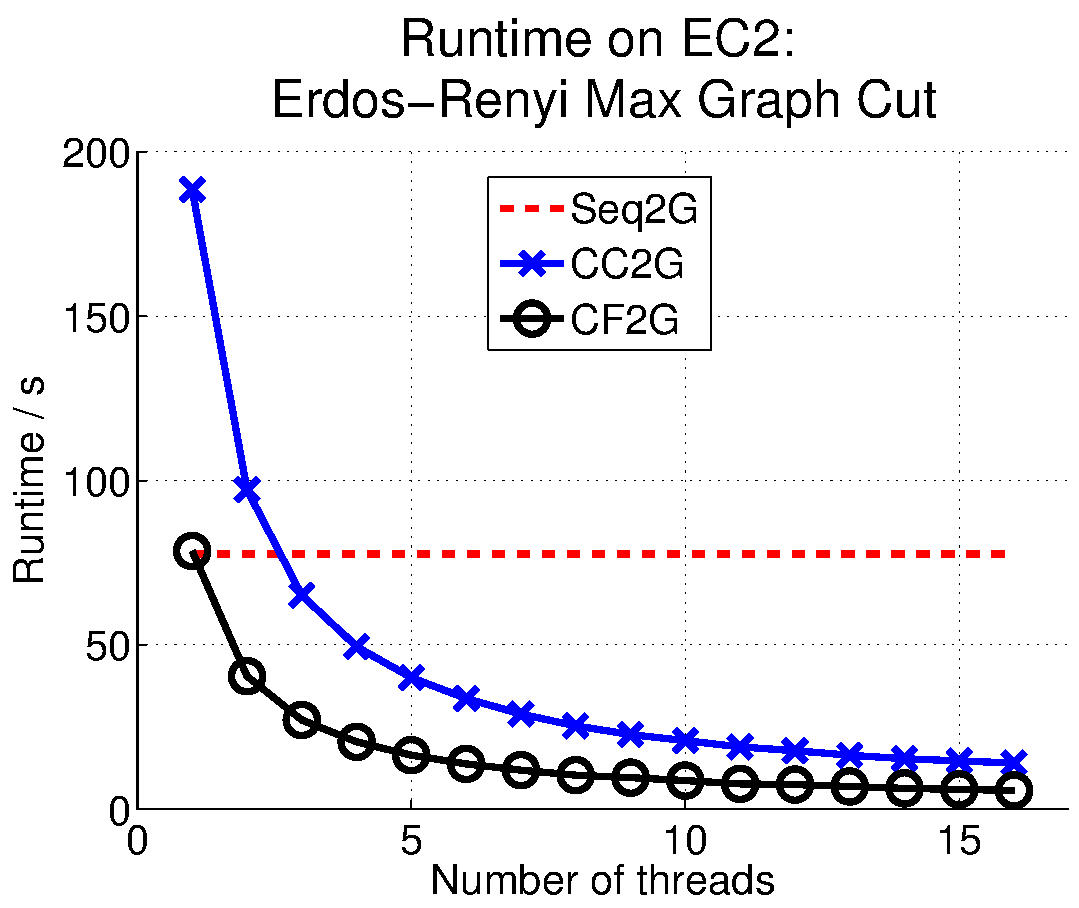
\includegraphics[width=110pt]{images/runtime_bigsynthetic_maxgraphcut.pdf}
			\caption{}
			\label{appfig:runtime_bigsynthetic_maxgraphcut}
	  \end{subfigure} &
	  \begin{subfigure}[b]{0.22\textwidth}
	  	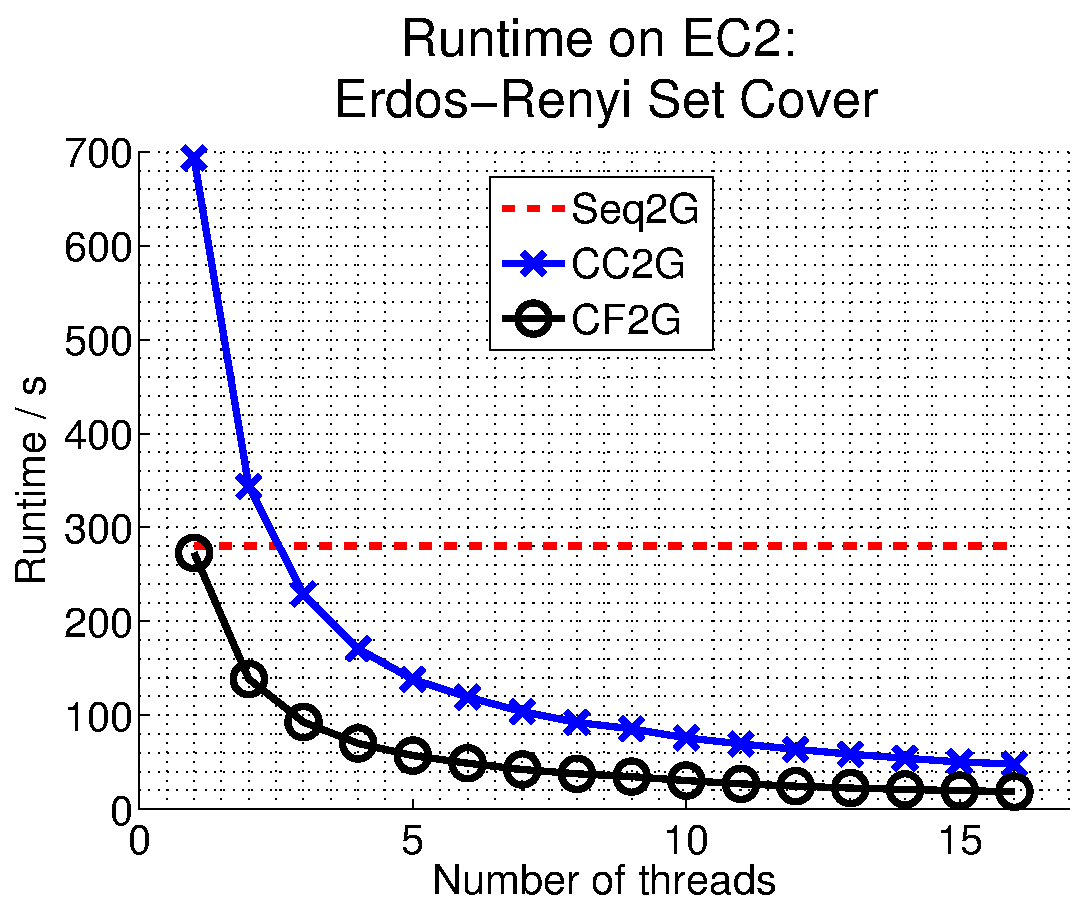
\includegraphics[width=110pt]{images/runtime_bigsynthetic_setcover.pdf}
			\caption{}
			\label{appfig:runtime_bigsynthetic_setcover}
	  \end{subfigure} &
	  \begin{subfigure}[b]{0.22\textwidth}
	  	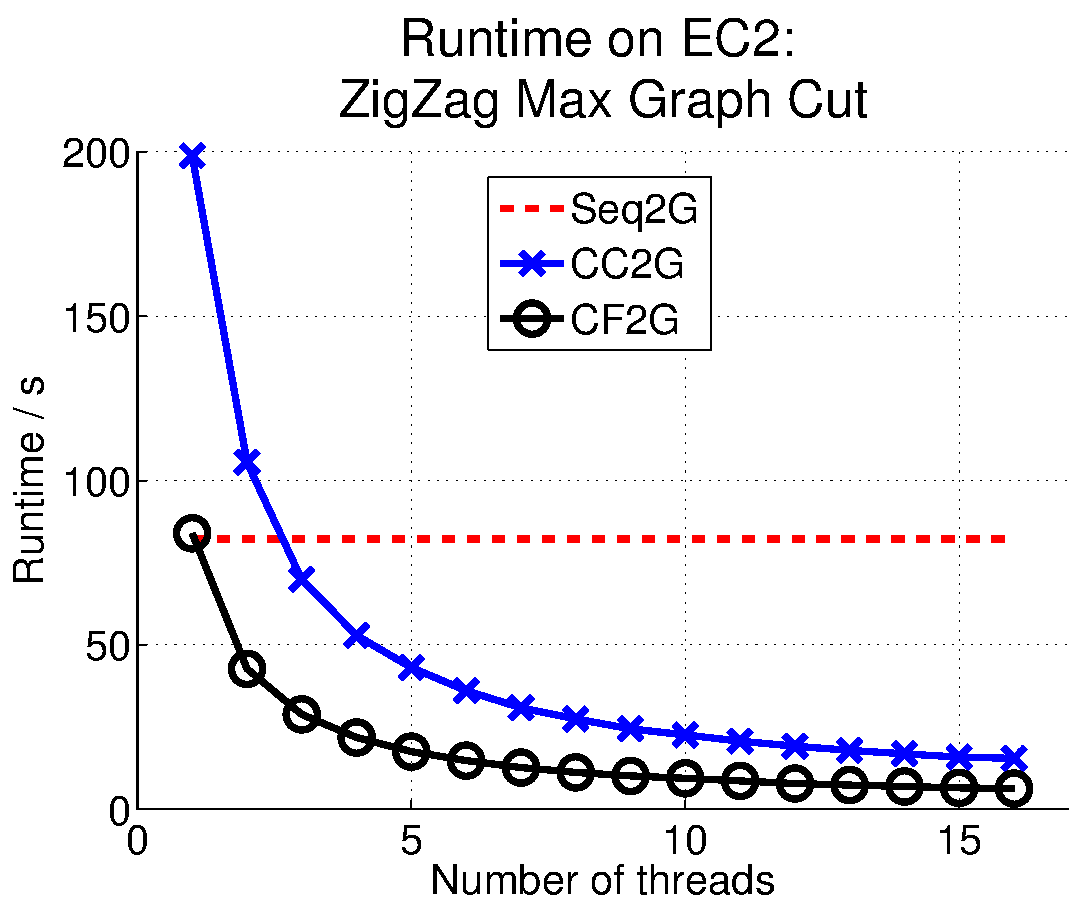
\includegraphics[width=110pt]{images/runtime_zigzag_maxgraphcut.pdf}
			\caption{}
			\label{appfig:runtime_zigzag_maxgraphcut}
	  \end{subfigure} &
	  \begin{subfigure}[b]{0.22\textwidth}
	  	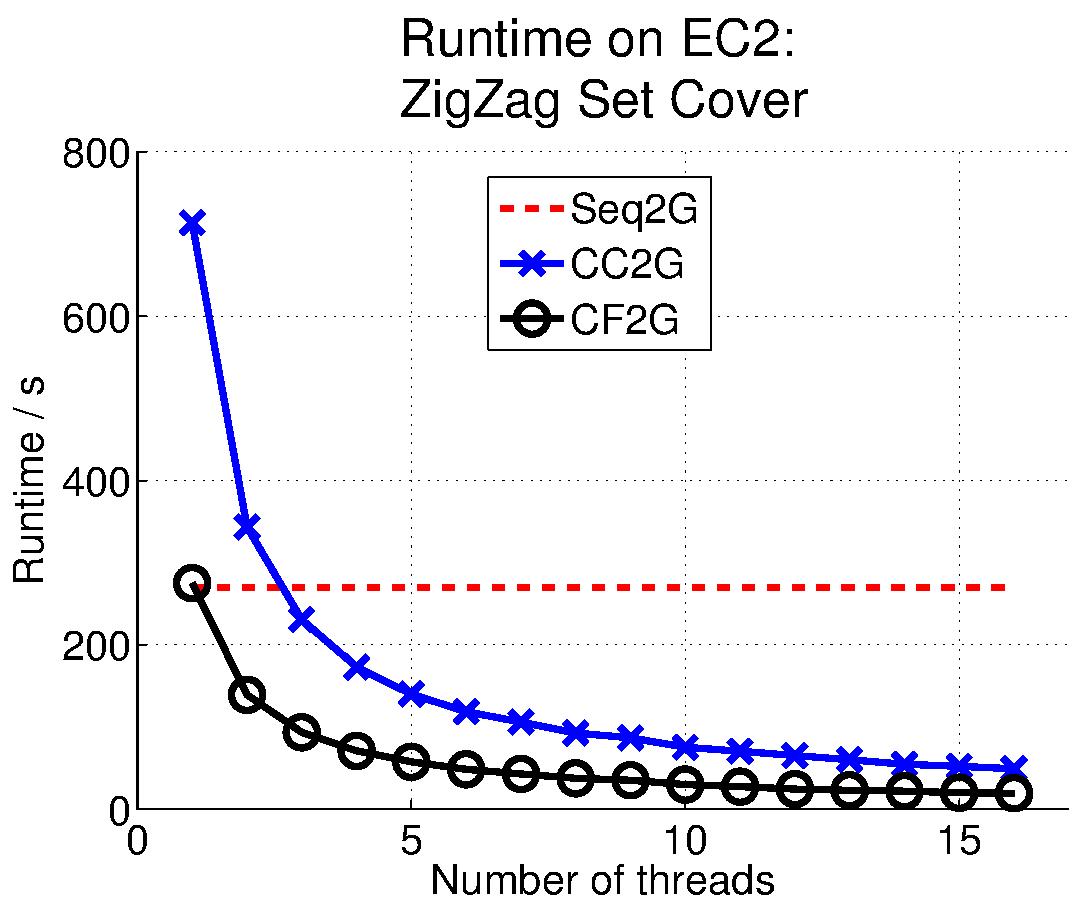
\includegraphics[width=110pt]{images/runtime_zigzag_setcover.pdf}
			\caption{}
			\label{appfig:runtime_zigzag_setcover}
	  \end{subfigure} \\
	  \begin{subfigure}[b]{0.22\textwidth}
	  	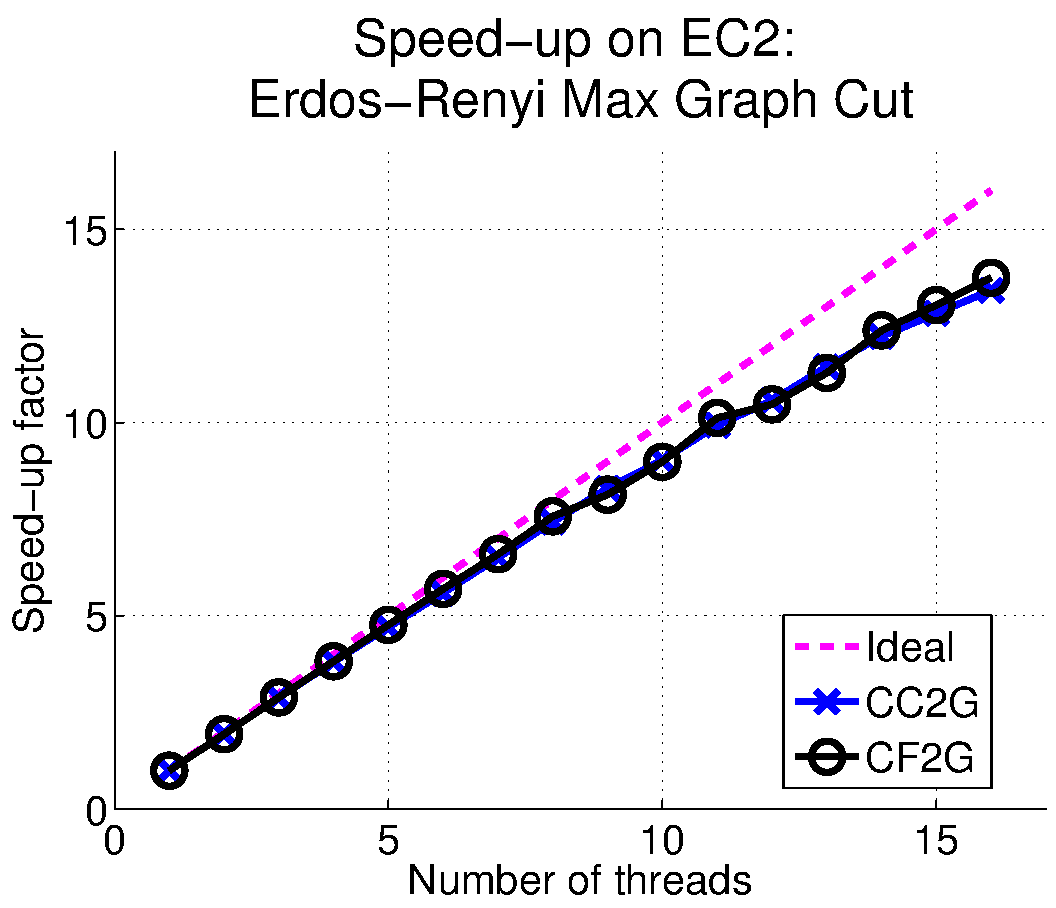
\includegraphics[width=110pt]{images/speedup_bigsynthetic_maxgraphcut.pdf}
			\caption{}
			\label{appfig:speedup_bigsynthetic_maxgraphcut}
	  \end{subfigure} &
	  \begin{subfigure}[b]{0.22\textwidth}
	  	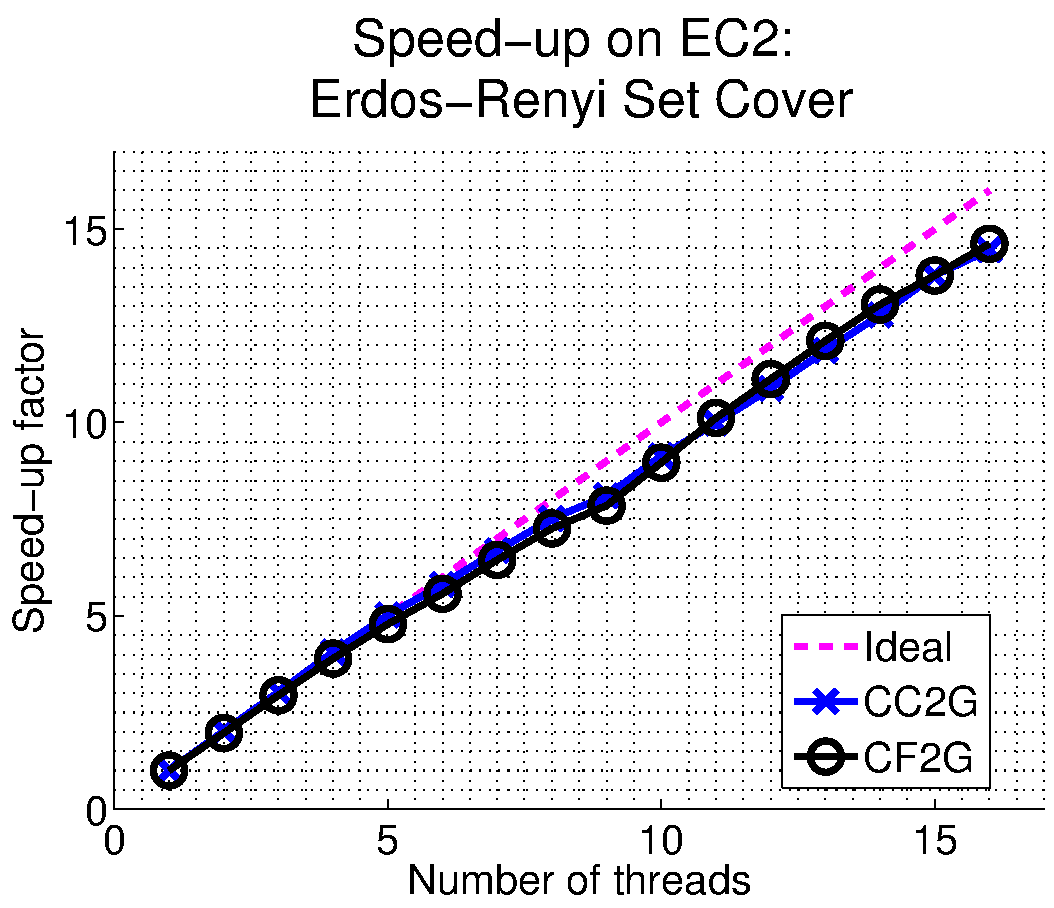
\includegraphics[width=110pt]{images/speedup_bigsynthetic_setcover.pdf}
			\caption{}
			\label{appfig:speedup_bigsynthetic_setcover}
	  \end{subfigure} &
	  \begin{subfigure}[b]{0.22\textwidth}
	  	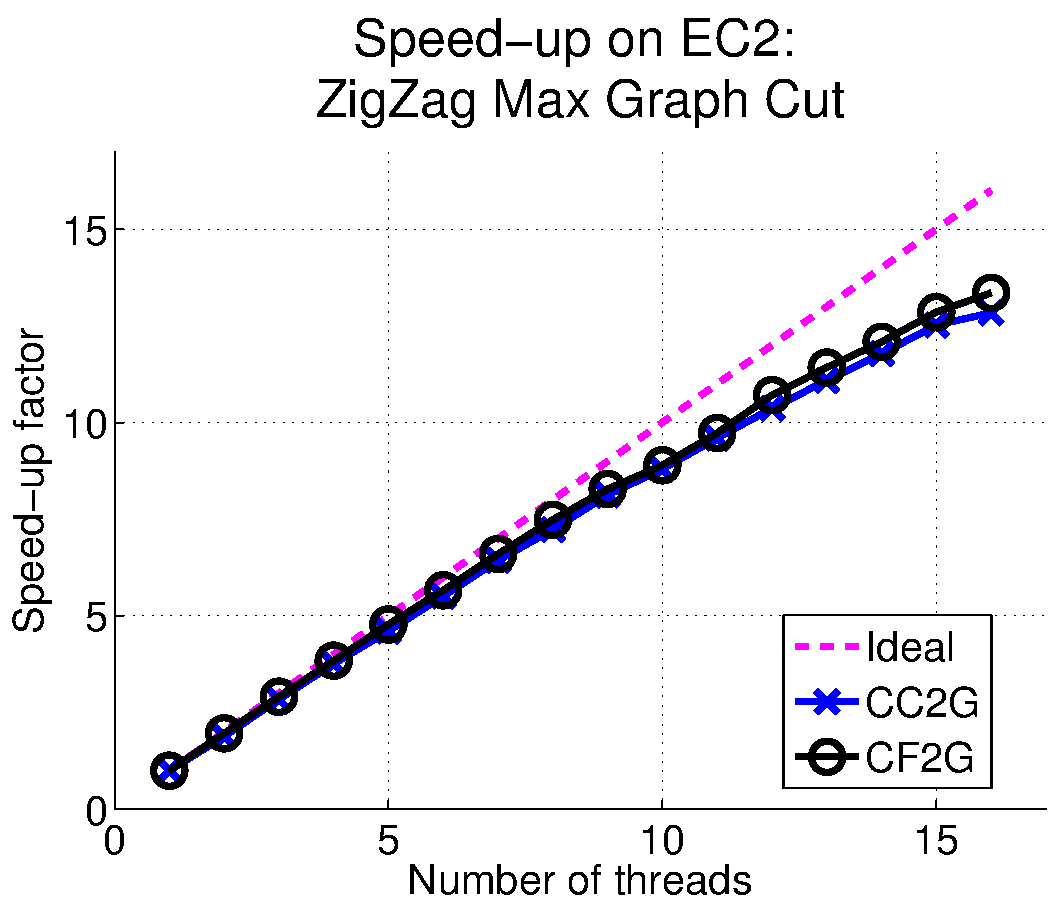
\includegraphics[width=110pt]{images/speedup_zigzag_maxgraphcut.pdf}
			\caption{}
			\label{appfig:speedup_zigzag_maxgraphcut}
	  \end{subfigure} &
	  \begin{subfigure}[b]{0.22\textwidth}
	  	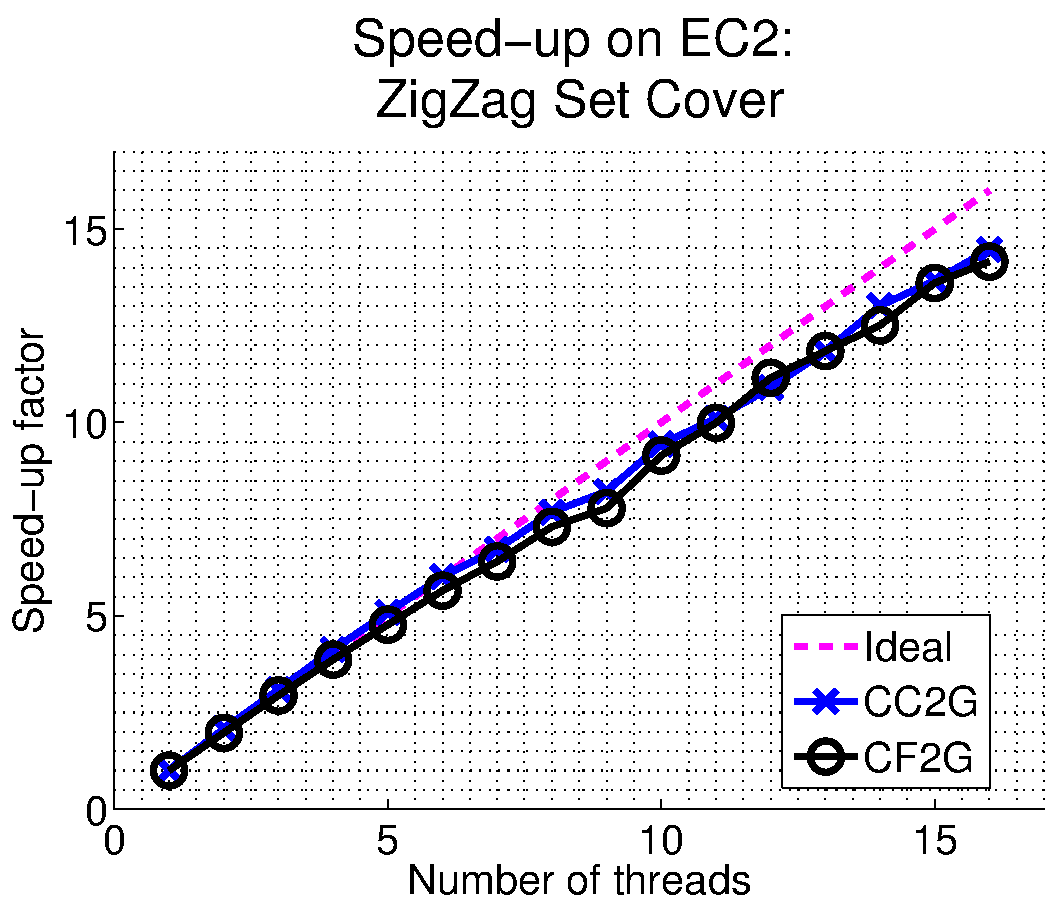
\includegraphics[width=110pt]{images/speedup_zigzag_setcover.pdf}
			\caption{}
			\label{appfig:speedup_zigzag_setcover}
	  \end{subfigure} \\
	  \begin{subfigure}[b]{0.22\textwidth}
	  	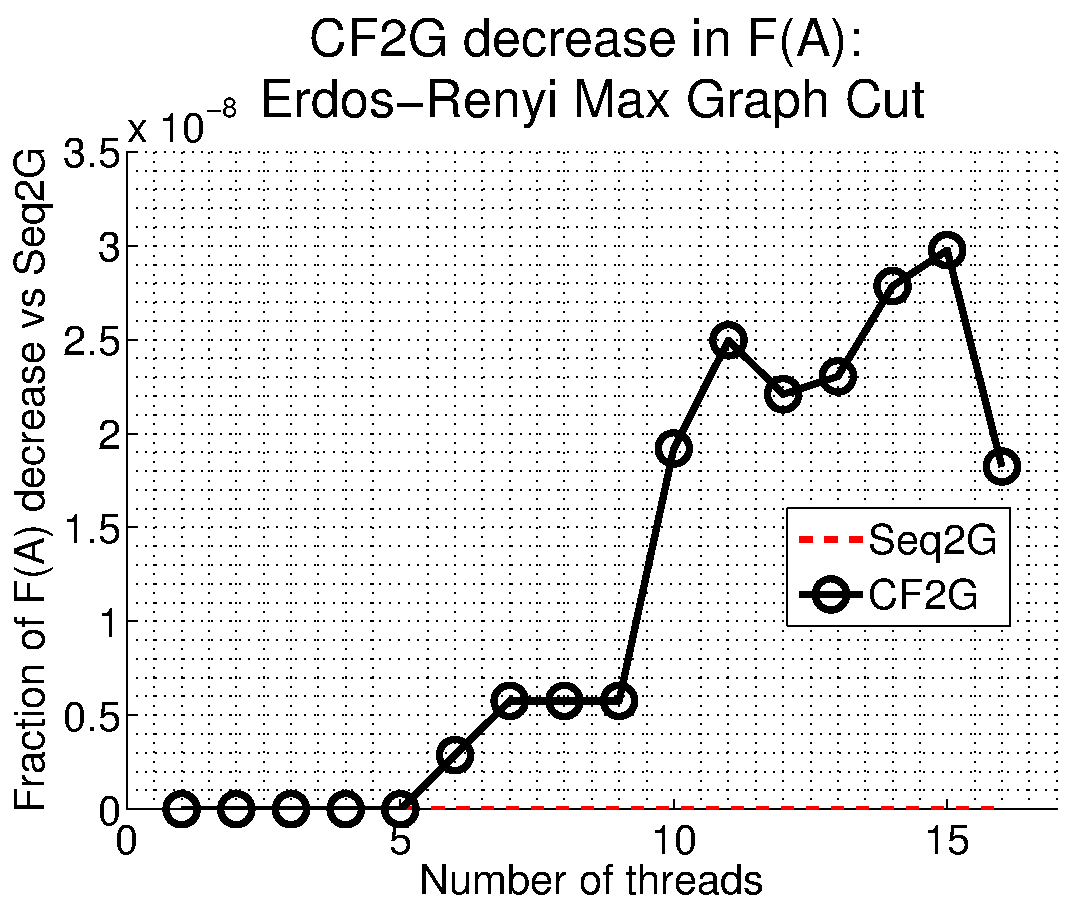
\includegraphics[width=110pt]{images/diffFA_CF2G_bigsynthetic_maxgraphcut.pdf}
			\caption{}
			\label{appfig:diffFA_CF2G_bigsynthetic_maxgraphcut}
	  \end{subfigure} &
	  \begin{subfigure}[b]{0.22\textwidth}
	  	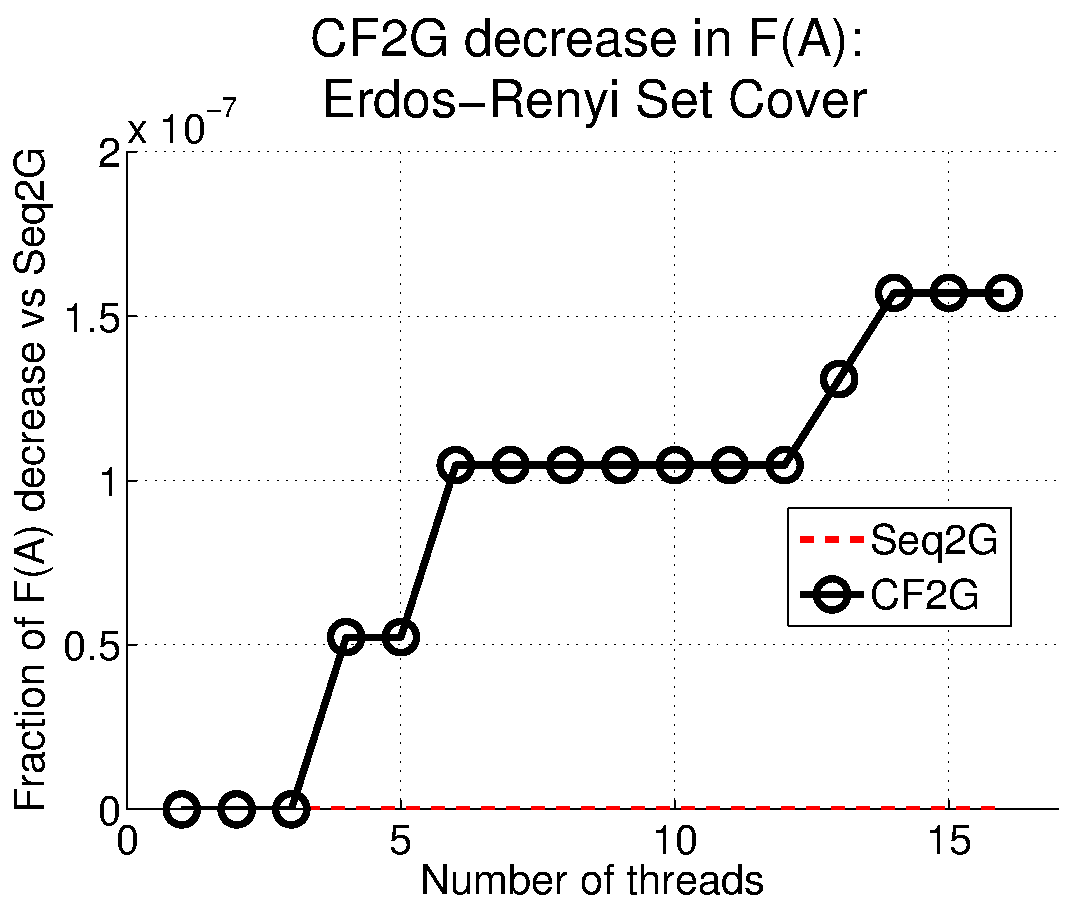
\includegraphics[width=110pt]{images/diffFA_CF2G_bigsynthetic_setcover.pdf}
			\caption{}
			\label{appfig:diffFA_CF2G_bigsynthetic_setcover}
	  \end{subfigure} &
	  \begin{subfigure}[b]{0.22\textwidth}
	  	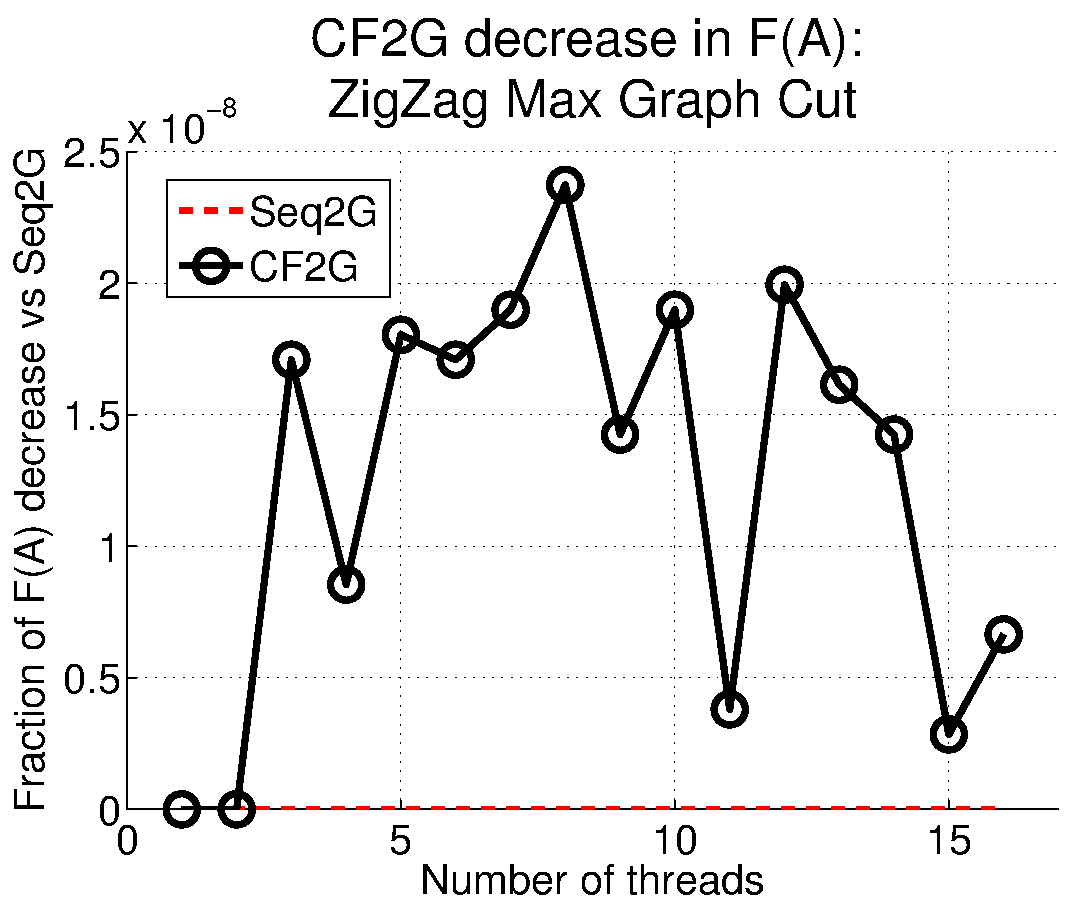
\includegraphics[width=110pt]{images/diffFA_CF2G_zigzag_maxgraphcut.pdf}
			\caption{}
			\label{appfig:diffFA_CF2G_zigzag_maxgraphcut}
	  \end{subfigure} &
	  \begin{subfigure}[b]{0.22\textwidth}
	  	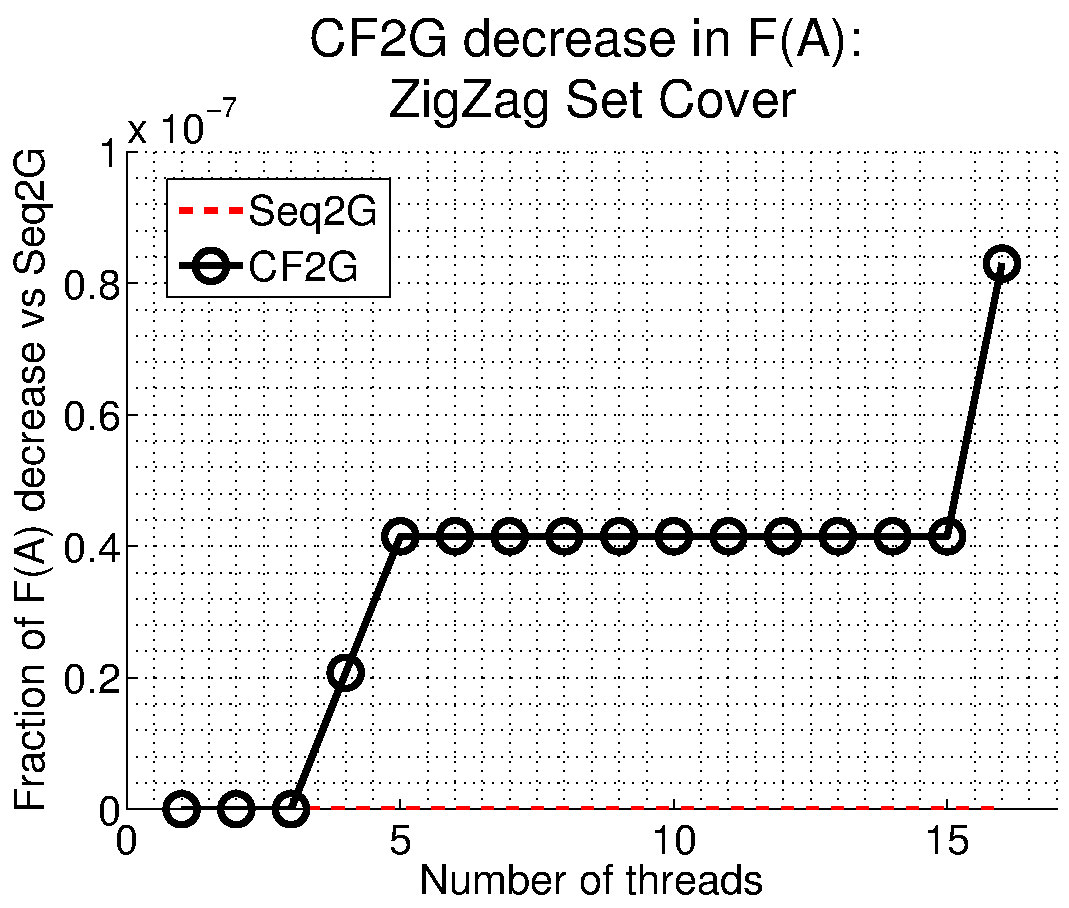
\includegraphics[width=110pt]{images/diffFA_CF2G_zigzag_setcover.pdf}
			\caption{}
			\label{appfig:diffFA_CF2G_zigzag_setcover}
	  \end{subfigure} \\
	  \begin{subfigure}[b]{0.22\textwidth}
	  	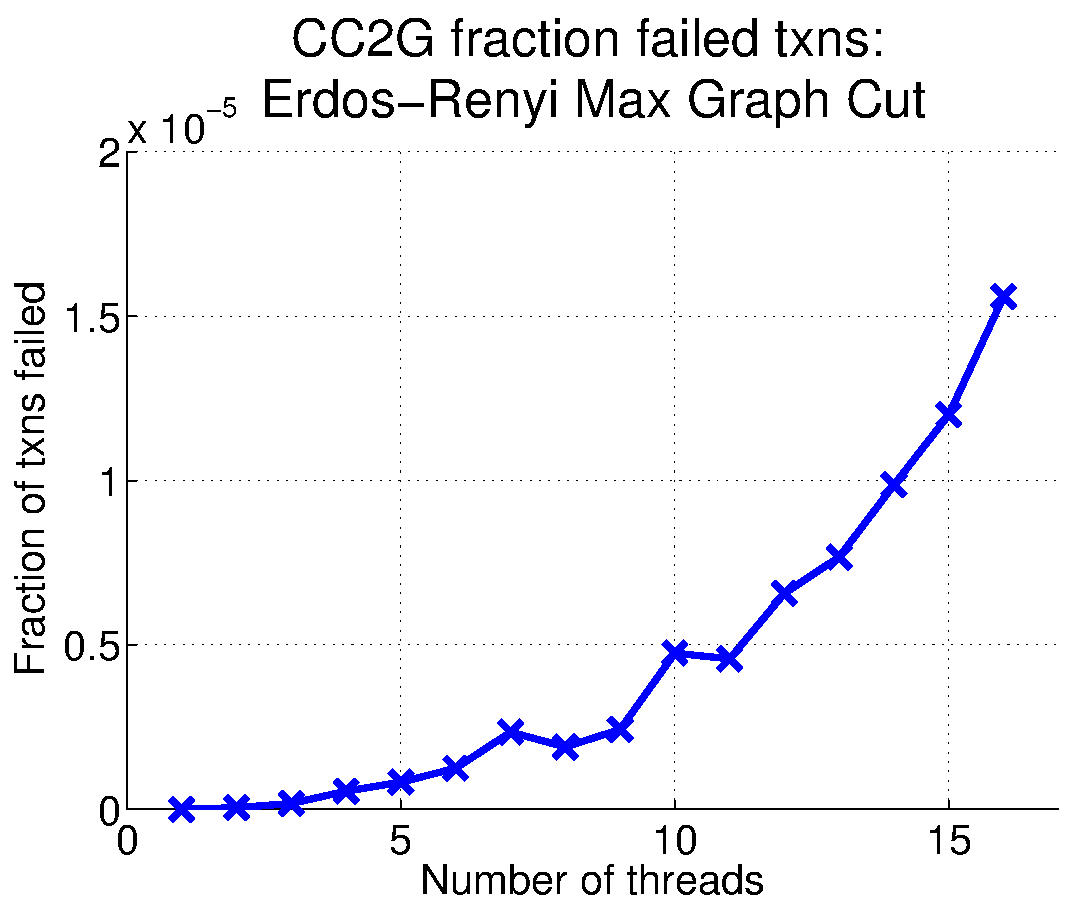
\includegraphics[width=110pt]{images/validated_CC2G_bigsynthetic_maxgraphcut.pdf}
			\caption{}
			\label{appfig:validated_CC2G_bigsynthetic_maxgraphcut}
	  \end{subfigure} &
	  \begin{subfigure}[b]{0.22\textwidth}
	  	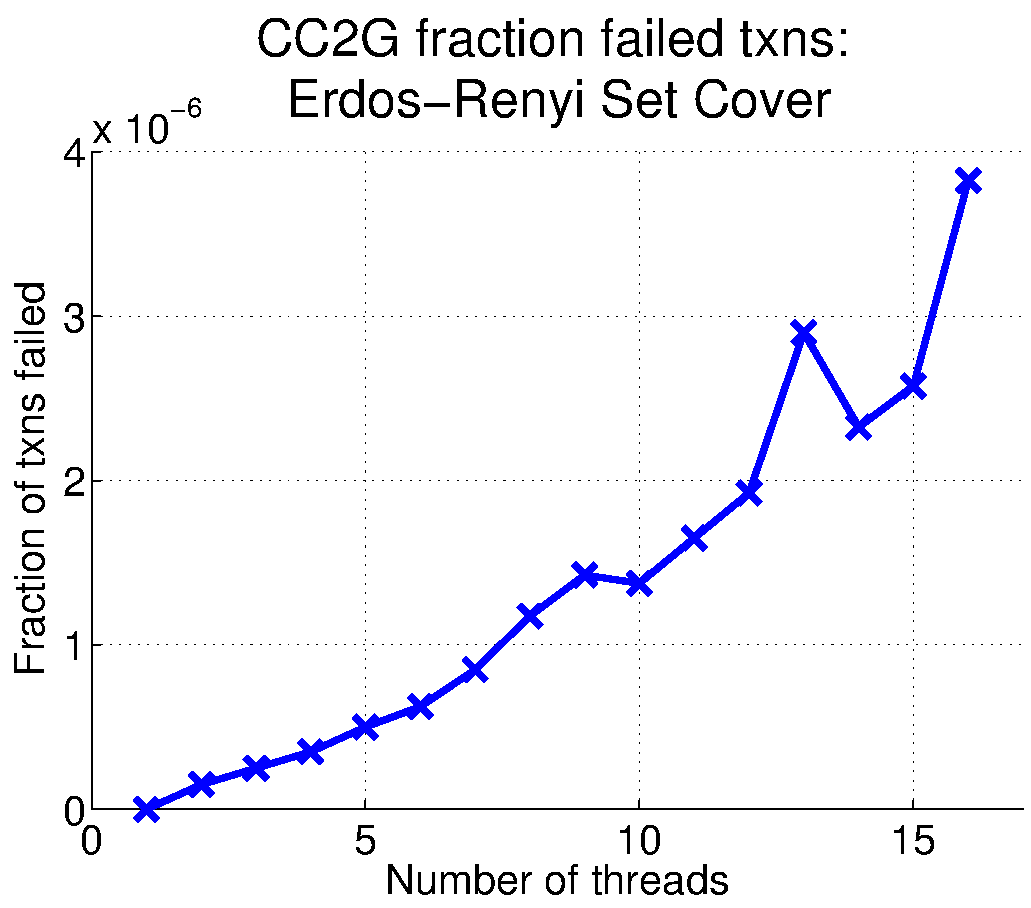
\includegraphics[width=110pt]{images/validated_CC2G_bigsynthetic_setcover.pdf}
			\caption{}
			\label{appfig:validated_CC2G_bigsynthetic_setcover}
	  \end{subfigure} &
	  \begin{subfigure}[b]{0.22\textwidth}
	  	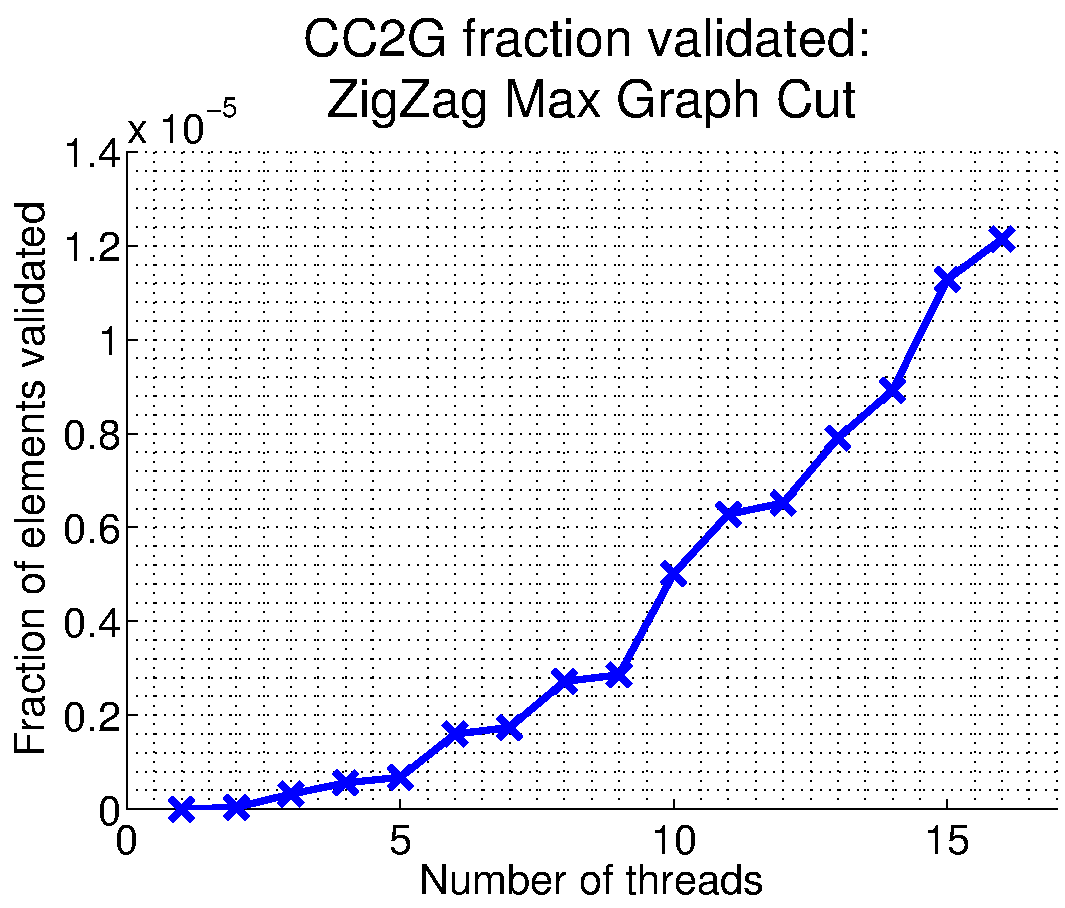
\includegraphics[width=110pt]{images/validated_CC2G_zigzag_maxgraphcut.pdf}
			\caption{}
			\label{appfig:validated_CC2G_zigzag_maxgraphcut}
	  \end{subfigure} &
	  \begin{subfigure}[b]{0.22\textwidth}
	  	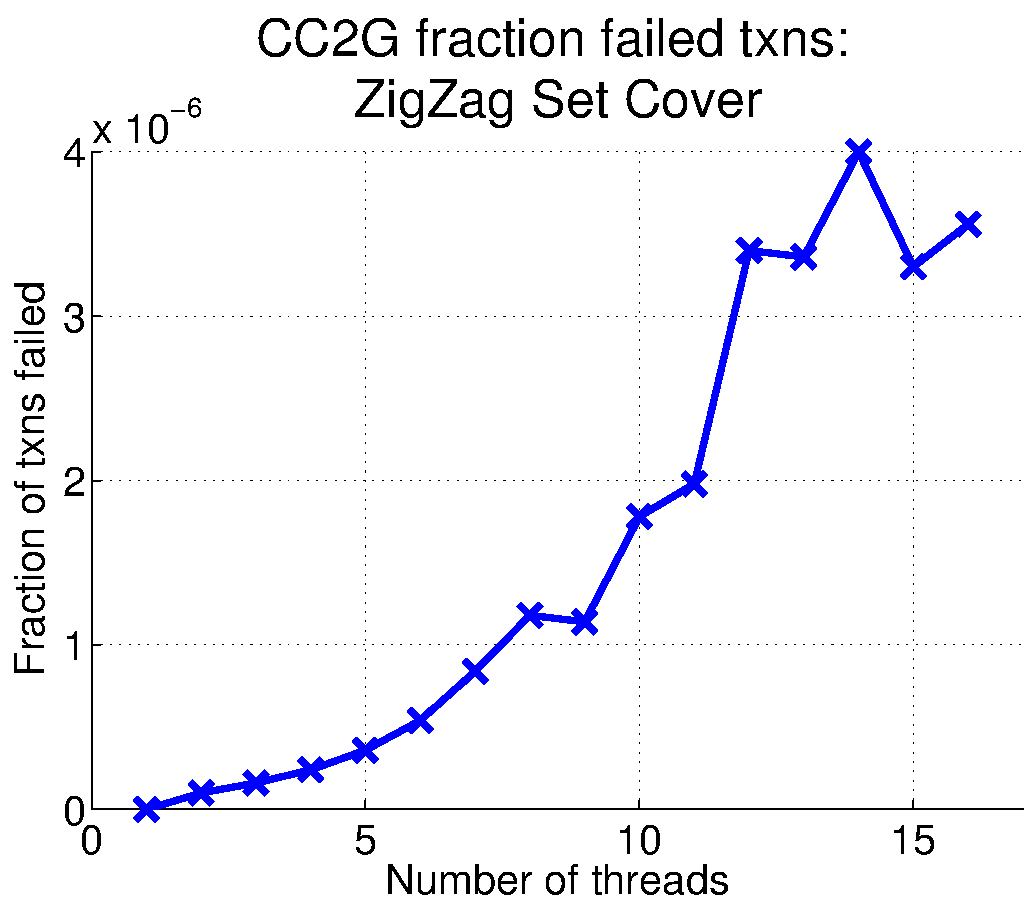
\includegraphics[width=110pt]{images/validated_CC2G_zigzag_setcover.pdf}
			\caption{}
			\label{appfig:validated_CC2G_zigzag_setcover}
	  \end{subfigure} \\
  \end{tabular}
  \caption{Experimental results on Erdos-Renyi and ZigZag synthetic graphs.}
\end{figure}


~\newpage\begin{figure}[ht]
  \centering
  \begin{tabular}{cccc}
	  \begin{subfigure}[b]{0.22\textwidth}
	  	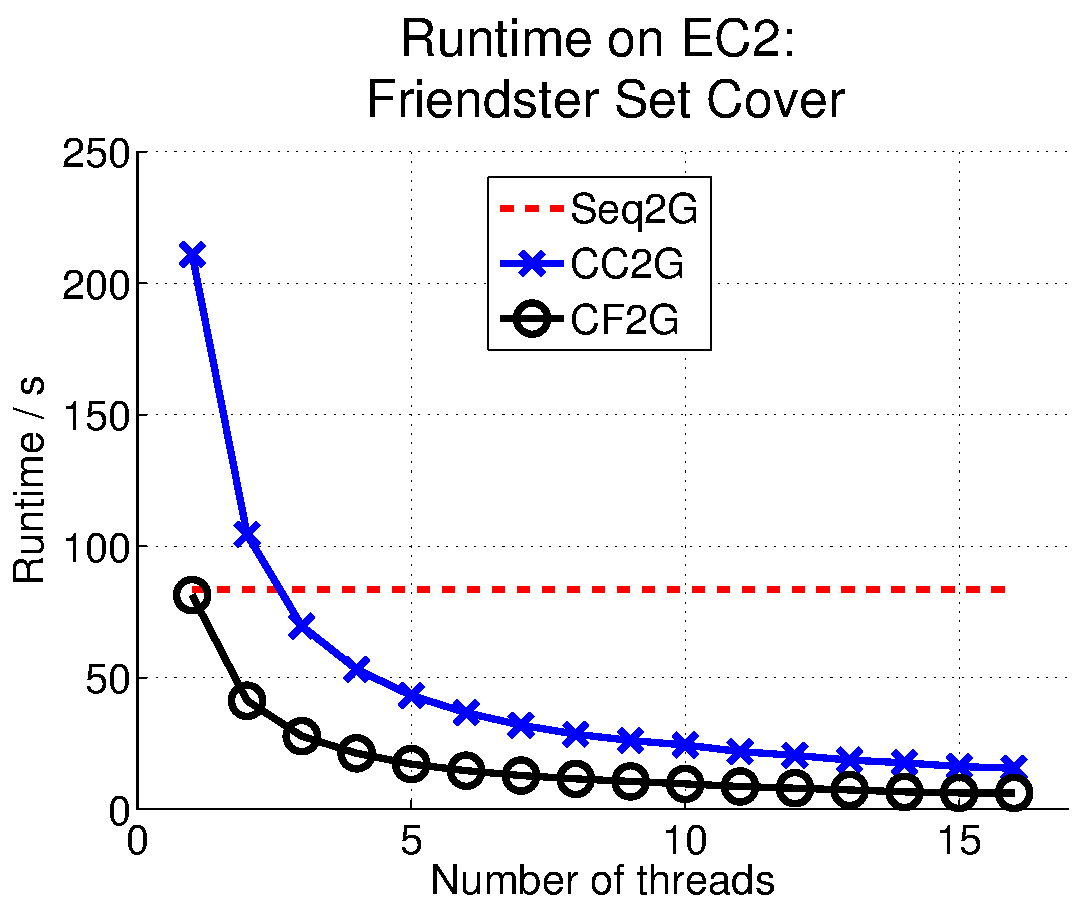
\includegraphics[width=110pt]{images/runtime_friendster10M_setcover.pdf}
			\caption{}
			\label{appfig:runtime_friendster10M_setcover}
	  \end{subfigure} &
	  \begin{subfigure}[b]{0.22\textwidth}
	  	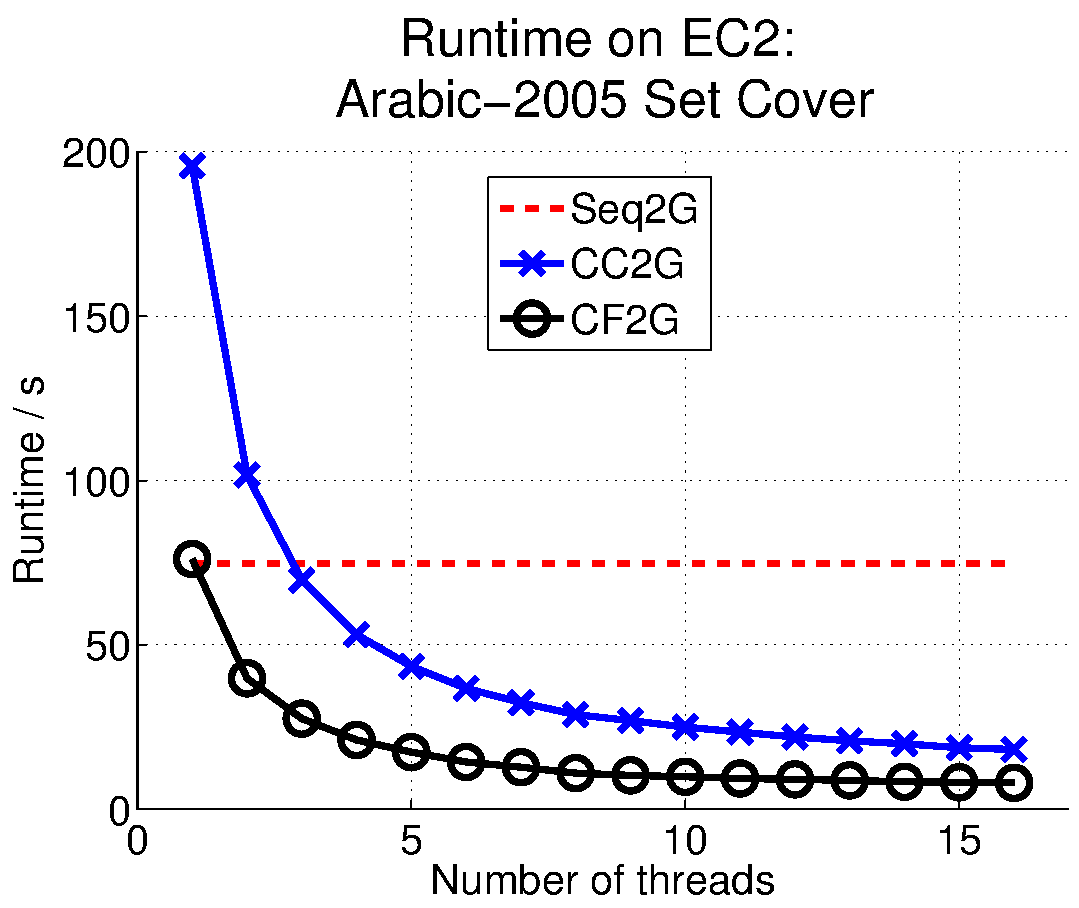
\includegraphics[width=110pt]{images/runtime_arabic2005_setcover.pdf}
			\caption{}
			\label{appfig:runtime_arabic2005_setcover}
	  \end{subfigure} &
	  \begin{subfigure}[b]{0.22\textwidth}
	  	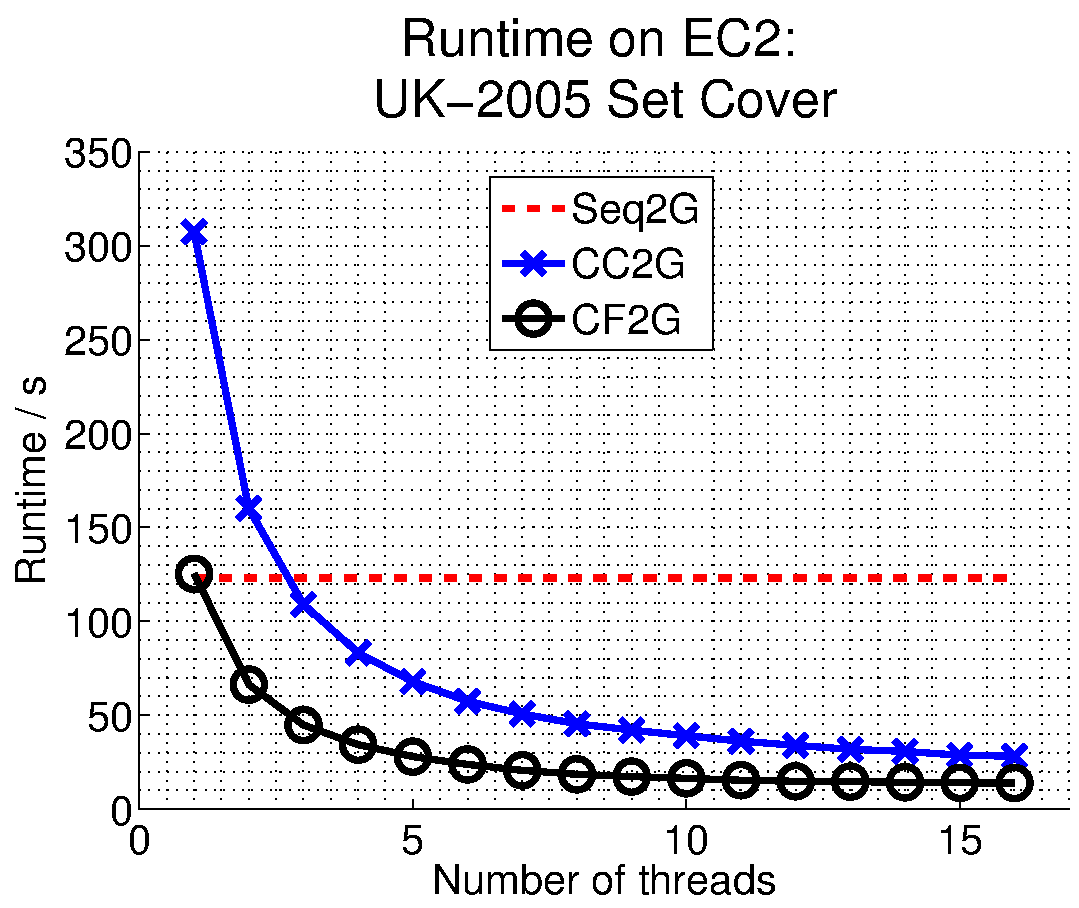
\includegraphics[width=110pt]{images/runtime_uk2005_setcover.pdf}
			\caption{}
			\label{appfig:runtime_uk2005_setcover}
	  \end{subfigure} &
	  \begin{subfigure}[b]{0.22\textwidth}
	  	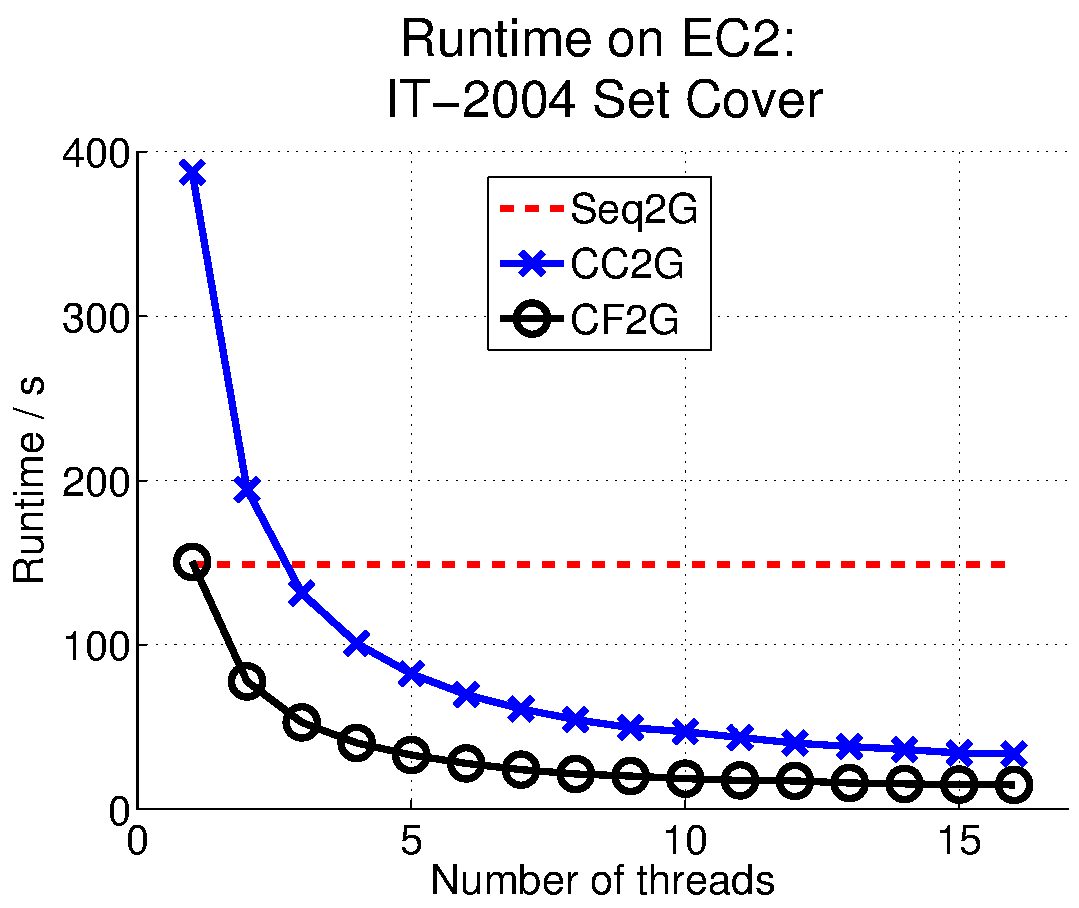
\includegraphics[width=110pt]{images/runtime_it2004_setcover.pdf}
			\caption{}
			\label{appfig:runtime_it2004_setcover}
	  \end{subfigure} \\
	  \begin{subfigure}[b]{0.22\textwidth}
	  	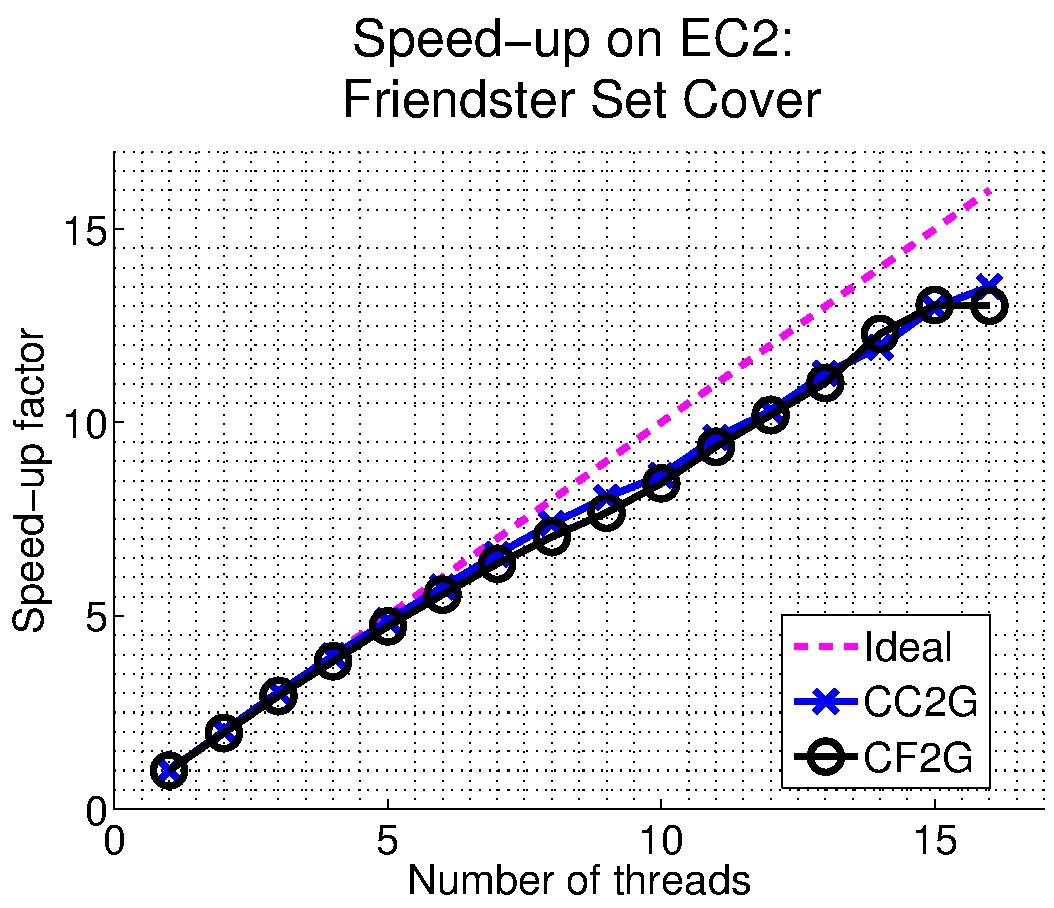
\includegraphics[width=110pt]{images/speedup_friendster10M_setcover.pdf}
			\caption{}
			\label{appfig:speedup_friendster10M_setcover}
	  \end{subfigure} &
	  \begin{subfigure}[b]{0.22\textwidth}
	  	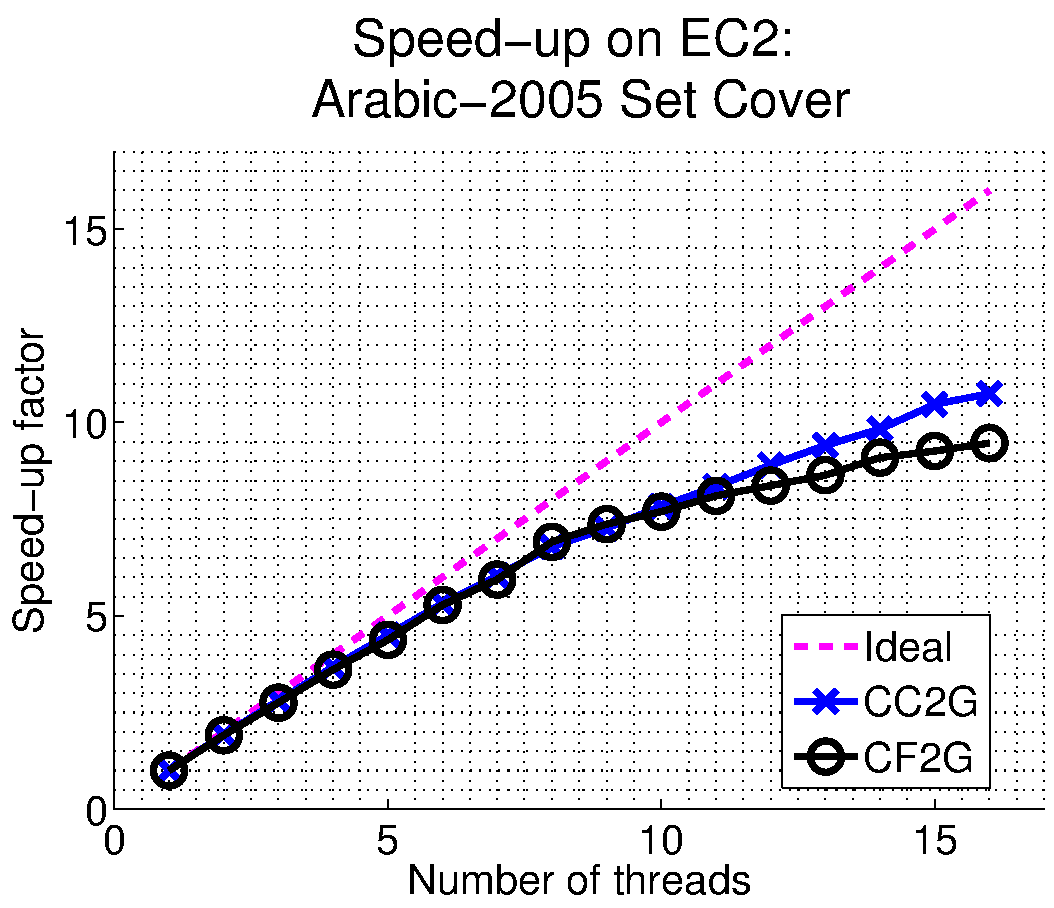
\includegraphics[width=110pt]{images/speedup_arabic2005_setcover.pdf}
			\caption{}
			\label{appfig:speedup_arabic2005_setcover}
	  \end{subfigure} &
	  \begin{subfigure}[b]{0.22\textwidth}
	  	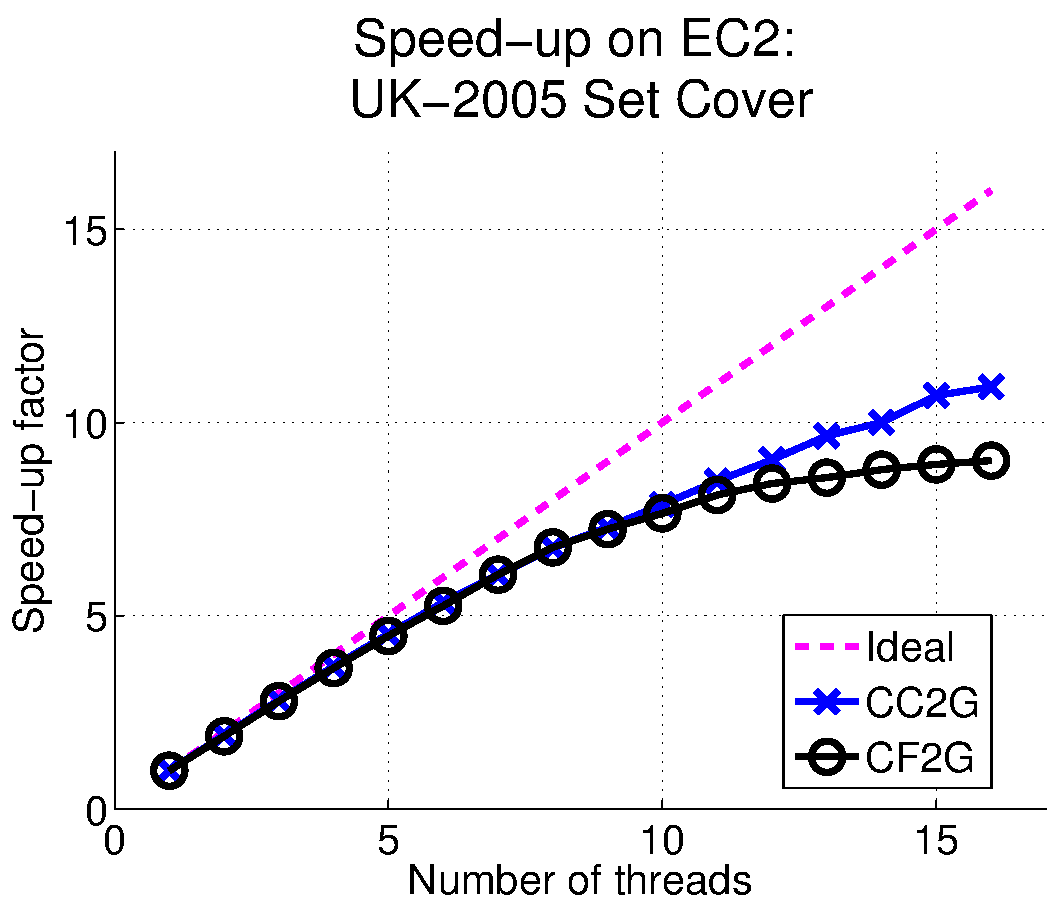
\includegraphics[width=110pt]{images/speedup_uk2005_setcover.pdf}
			\caption{}
			\label{appfig:speedup_uk2005_setcover}
	  \end{subfigure} &
	  \begin{subfigure}[b]{0.22\textwidth}
	  	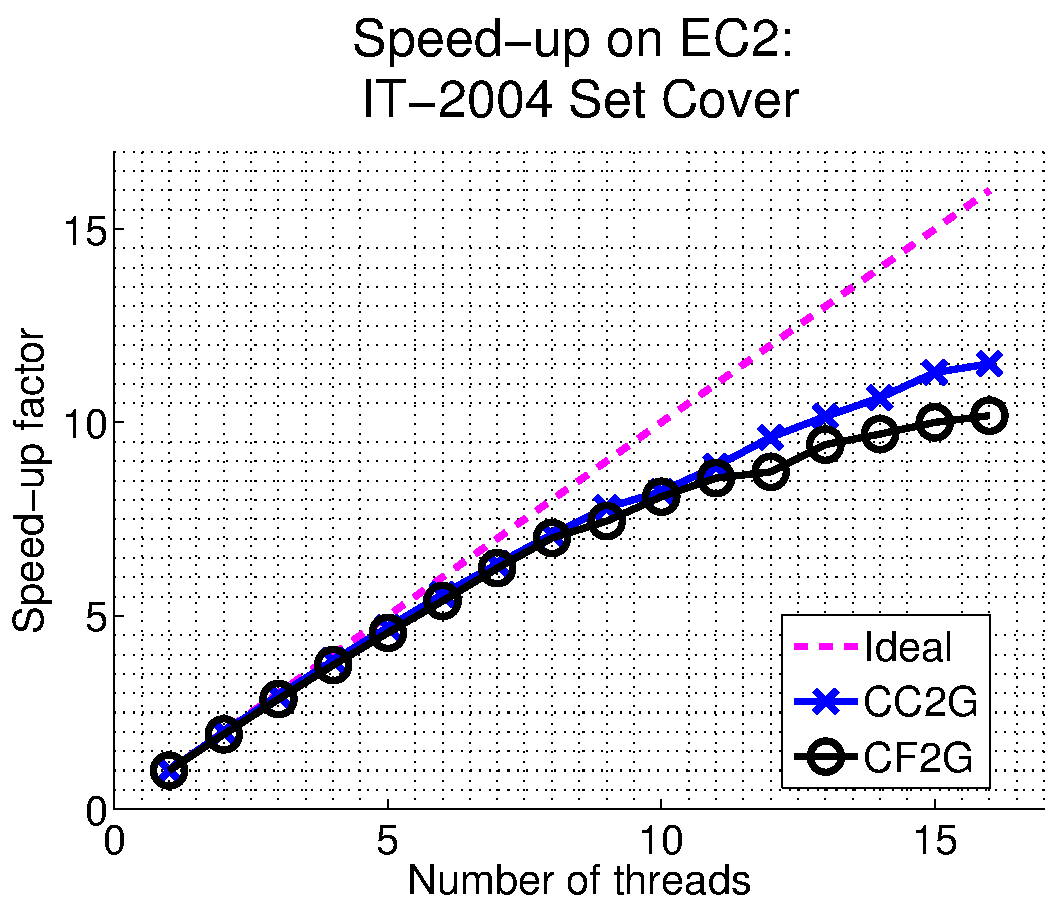
\includegraphics[width=110pt]{images/speedup_it2004_setcover.pdf}
			\caption{}
			\label{appfig:speedup_it2004_setcover}
	  \end{subfigure} \\
	  \begin{subfigure}[b]{0.22\textwidth}
	  	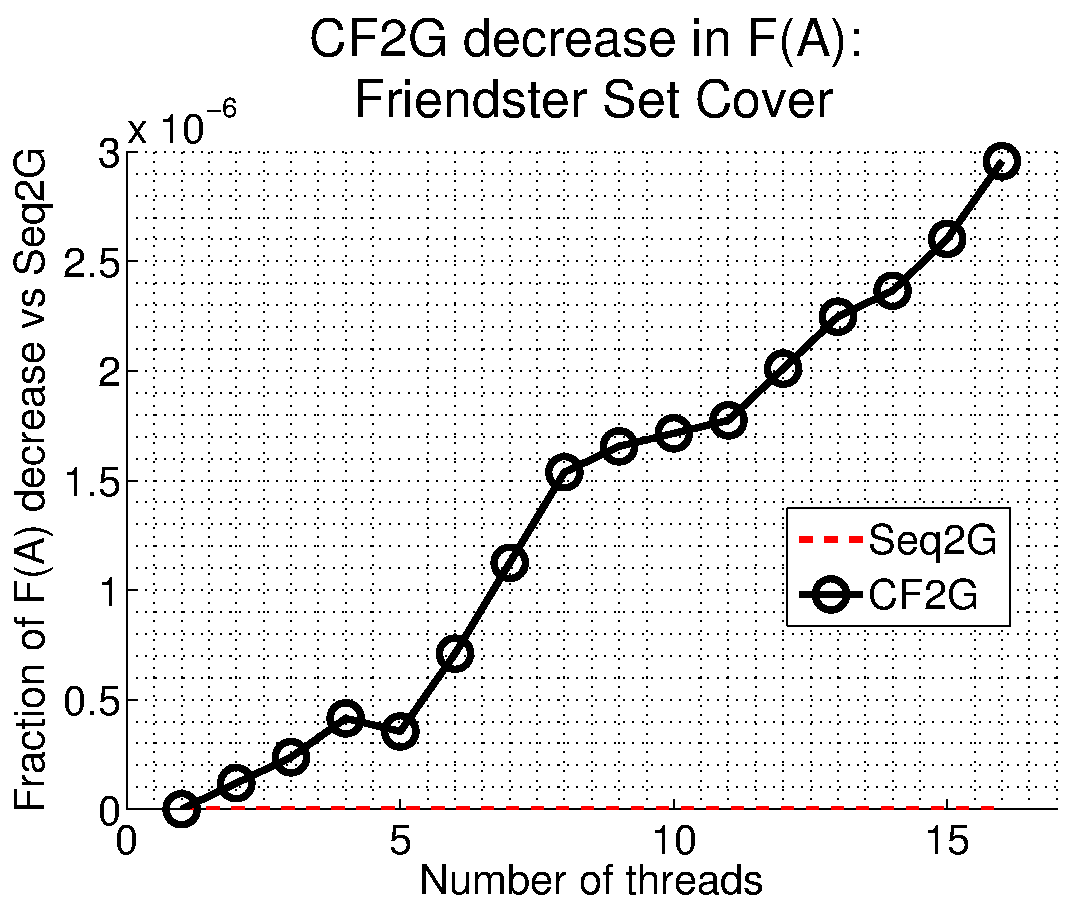
\includegraphics[width=110pt]{images/diffFA_CF2G_friendster10M_setcover.pdf}
			\caption{}
			\label{appfig:diffFA_CF2G_friendster10M_setcover}
	  \end{subfigure} &
	  \begin{subfigure}[b]{0.22\textwidth}
	  	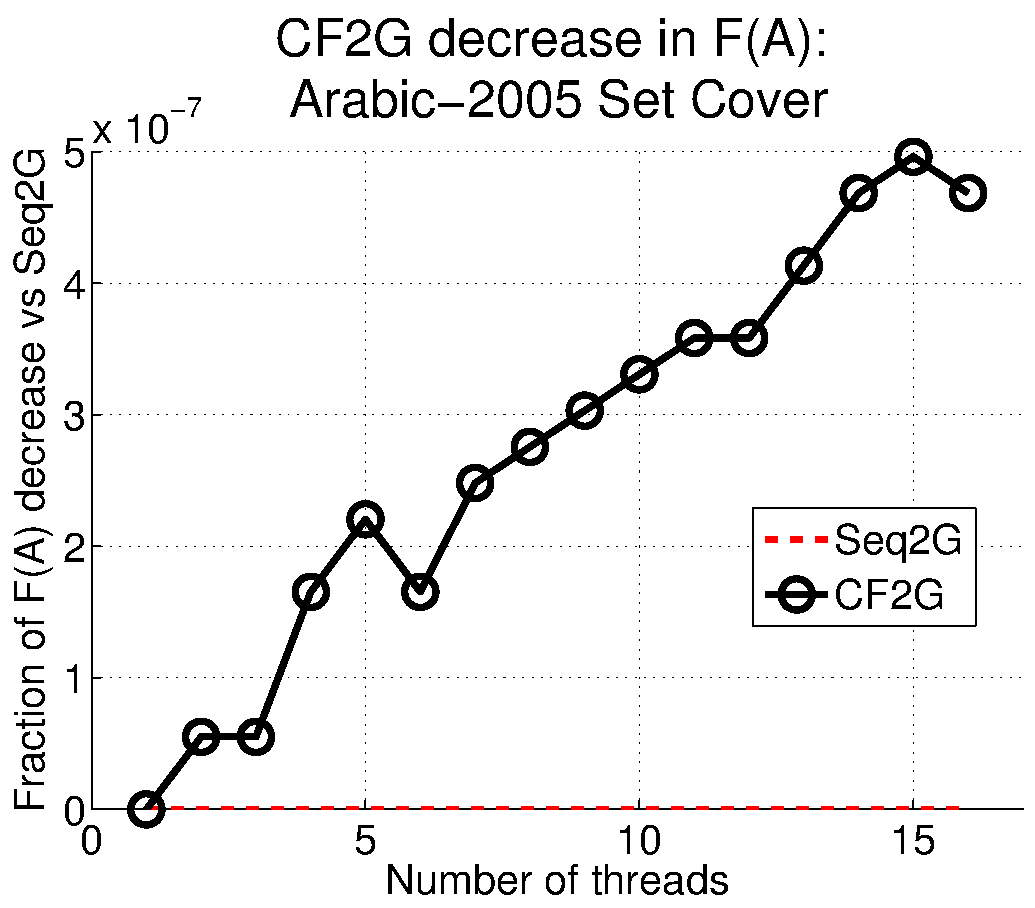
\includegraphics[width=110pt]{images/diffFA_CF2G_arabic2005_setcover.pdf}
			\caption{}
			\label{appfig:diffFA_CF2G_arabic2005_setcover}
	  \end{subfigure} &
	  \begin{subfigure}[b]{0.22\textwidth}
	  	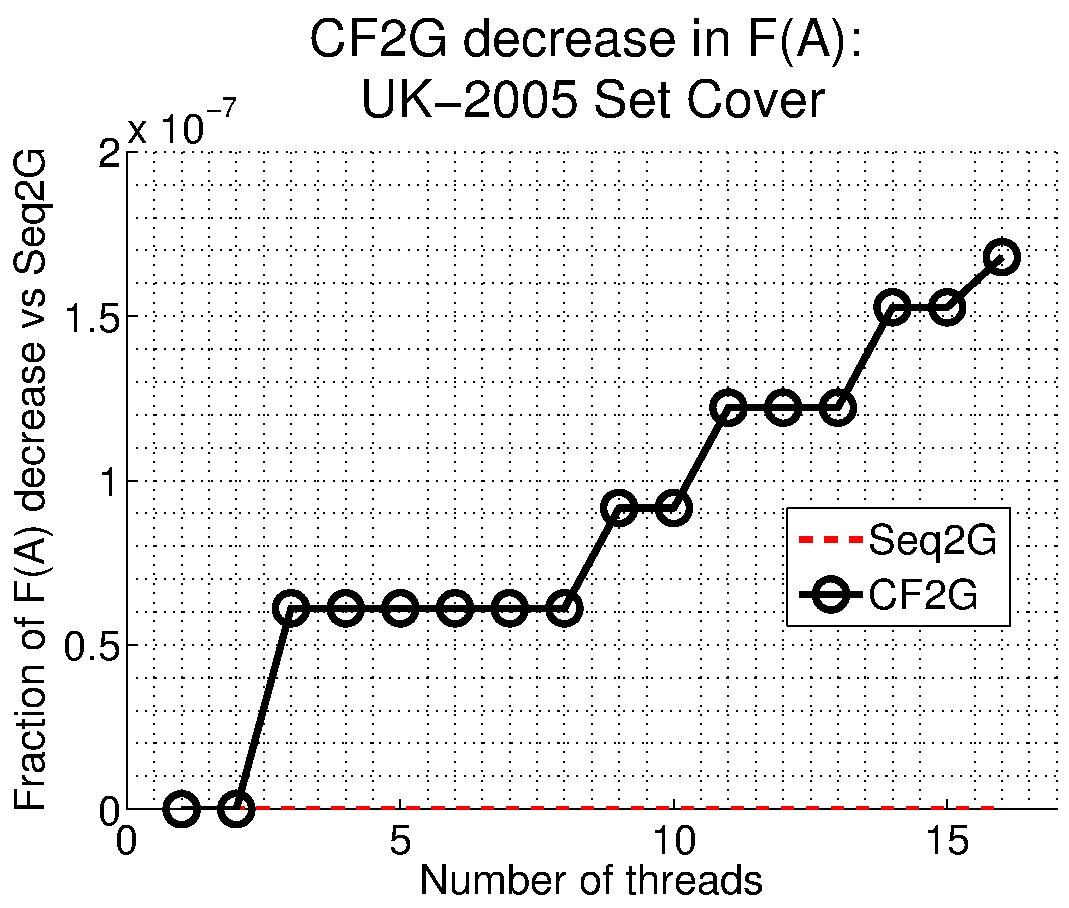
\includegraphics[width=110pt]{images/diffFA_CF2G_uk2005_setcover.pdf}
			\caption{}
			\label{appfig:diffFA_CF2G_uk2005_setcover}
	  \end{subfigure} &
	  \begin{subfigure}[b]{0.22\textwidth}
	  	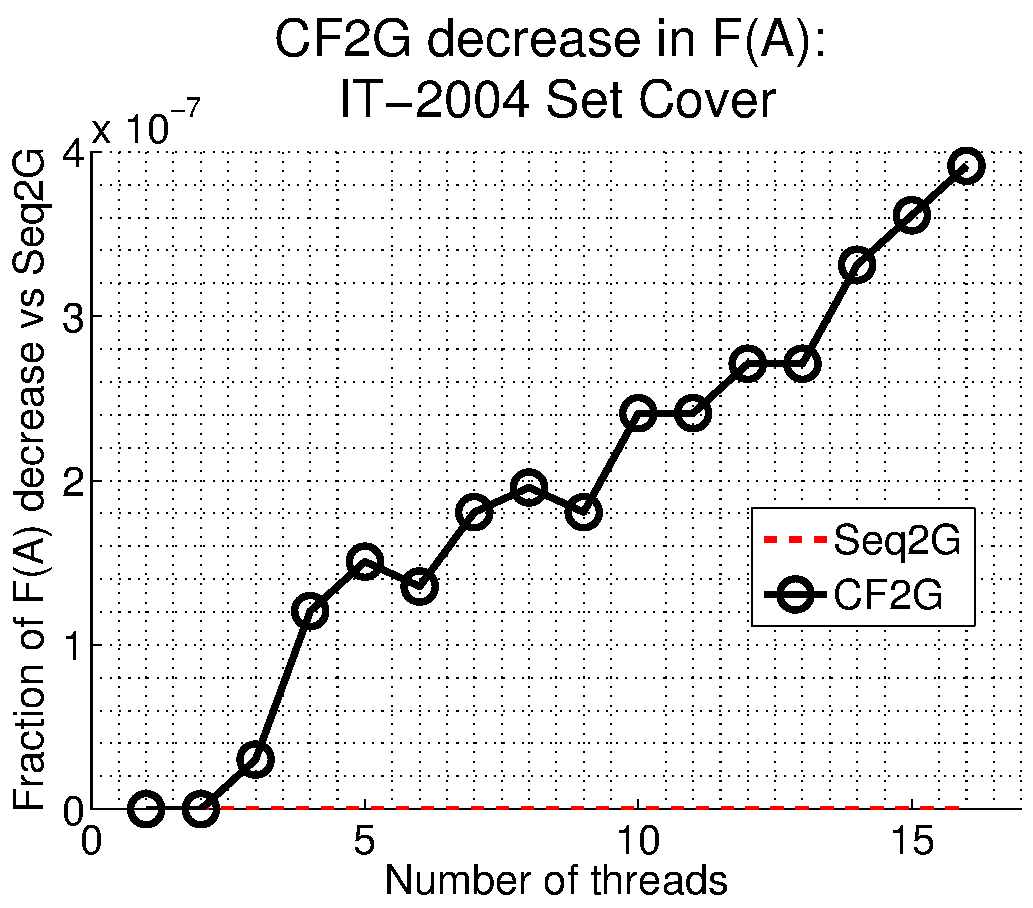
\includegraphics[width=110pt]{images/diffFA_CF2G_it2004_setcover.pdf}
			\caption{}
			\label{appfig:diffFA_CF2G_it2004_setcover}
	  \end{subfigure} \\
	  \begin{subfigure}[b]{0.22\textwidth}
	  	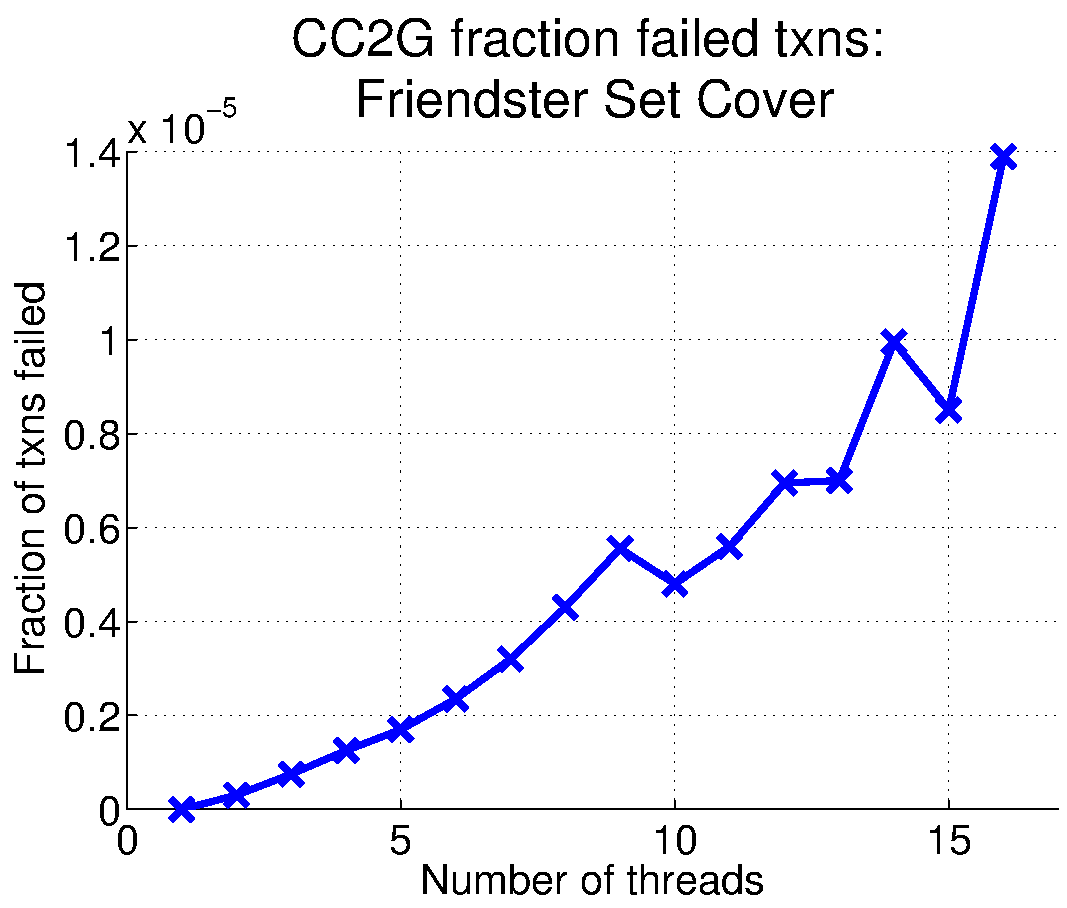
\includegraphics[width=110pt]{images/validated_CC2G_friendster10M_setcover.pdf}
			\caption{}
			\label{appfig:validated_CC2G_friendster10M_setcover}
	  \end{subfigure} &
	  \begin{subfigure}[b]{0.22\textwidth}
	  	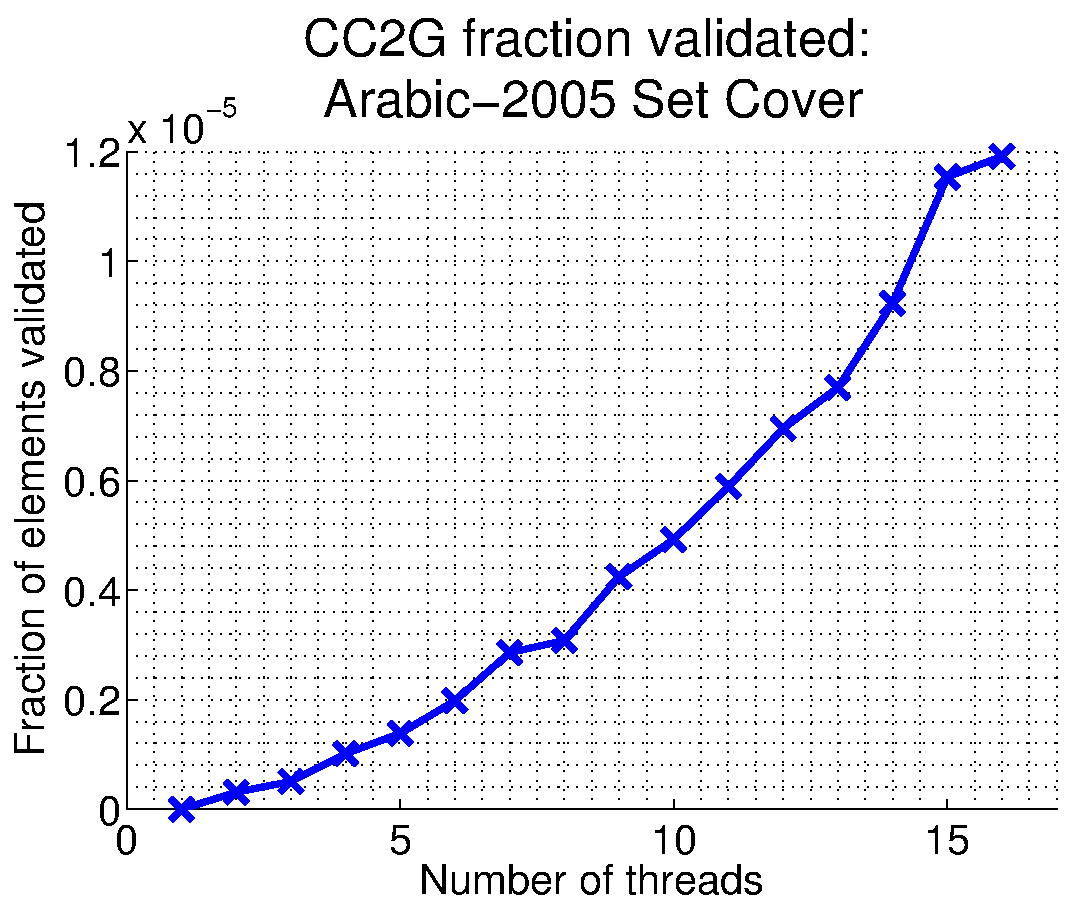
\includegraphics[width=110pt]{images/validated_CC2G_arabic2005_setcover.pdf}
			\caption{}
			\label{appfig:validated_CC2G_arabic2005_setcover}
	  \end{subfigure} &
	  \begin{subfigure}[b]{0.22\textwidth}
	  	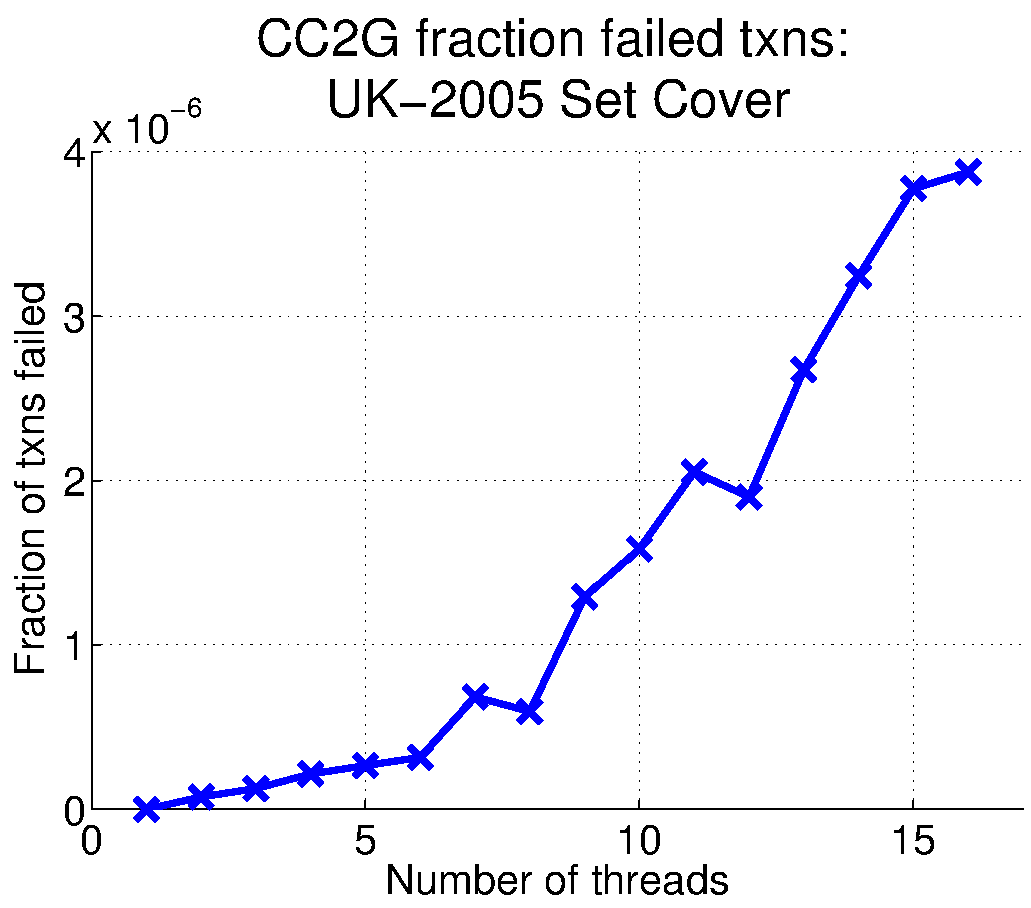
\includegraphics[width=110pt]{images/validated_CC2G_uk2005_setcover.pdf}
			\caption{}
			\label{appfig:validated_CC2G_uk2005_setcover}
	  \end{subfigure} &
	  \begin{subfigure}[b]{0.22\textwidth}
	  	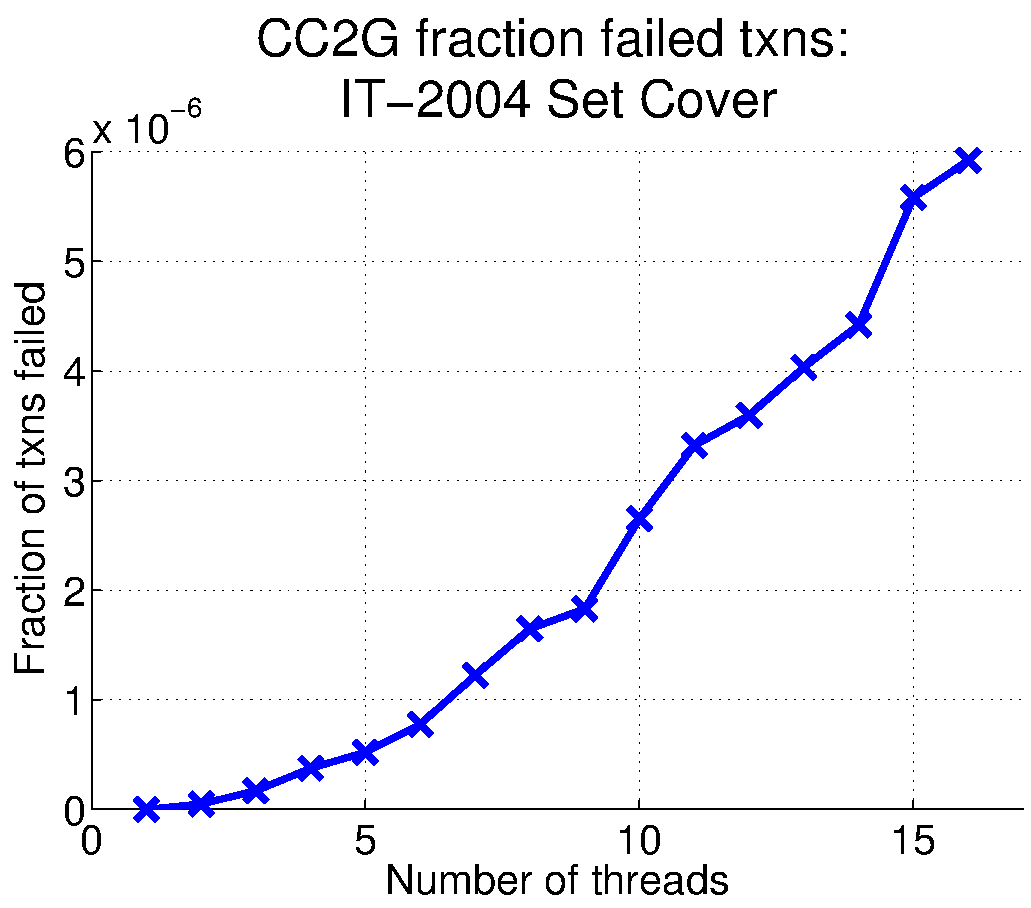
\includegraphics[width=110pt]{images/validated_CC2G_it2004_setcover.pdf}
			\caption{}
			\label{appfig:validated_CC2G_it2004_setcover}
	  \end{subfigure} \\
  \end{tabular}
  \caption{Set cover on 4 real graphs.}
\end{figure}



~\newpage\begin{figure}[ht]
  \centering
  \begin{tabular}{cccc}
	  \begin{subfigure}[b]{0.22\textwidth}
	  	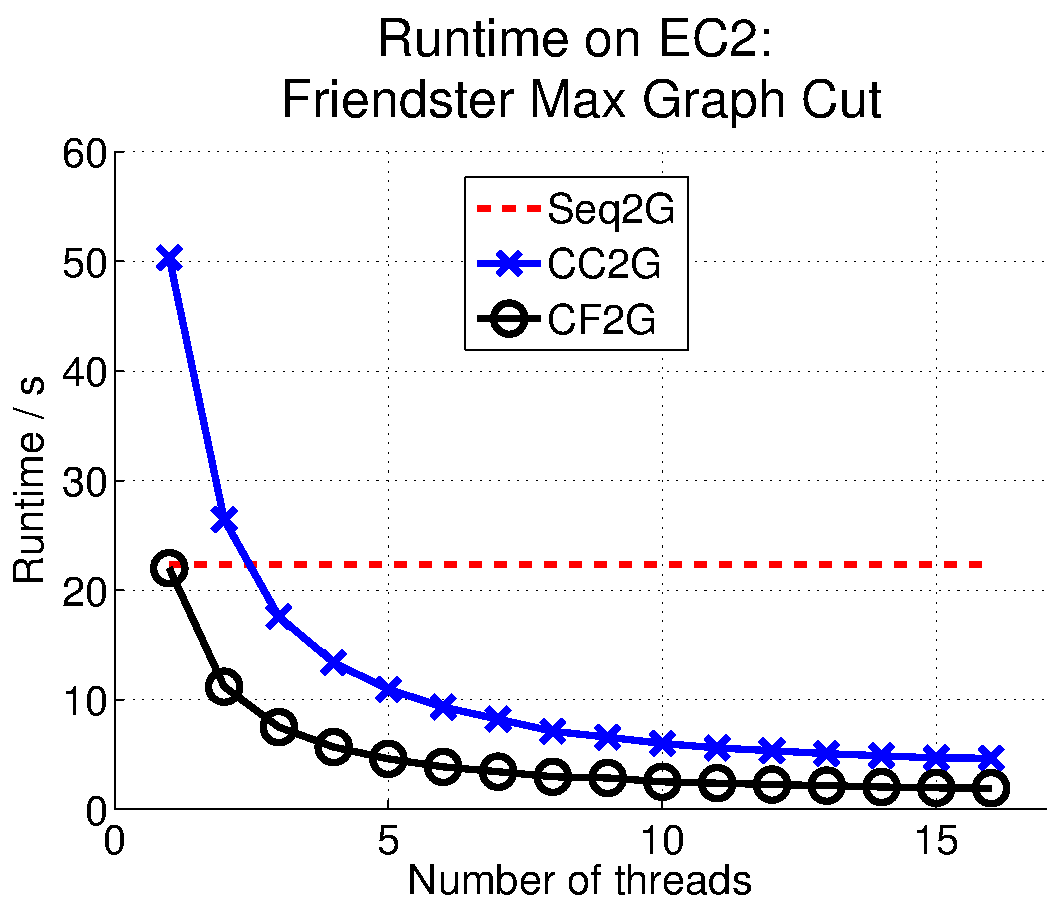
\includegraphics[width=110pt]{images/runtime_friendster10M_maxgraphcut.pdf}
			\caption{}
			\label{appfig:runtime_friendster10M_maxgraphcut}
	  \end{subfigure} &
	  \begin{subfigure}[b]{0.22\textwidth}
	  	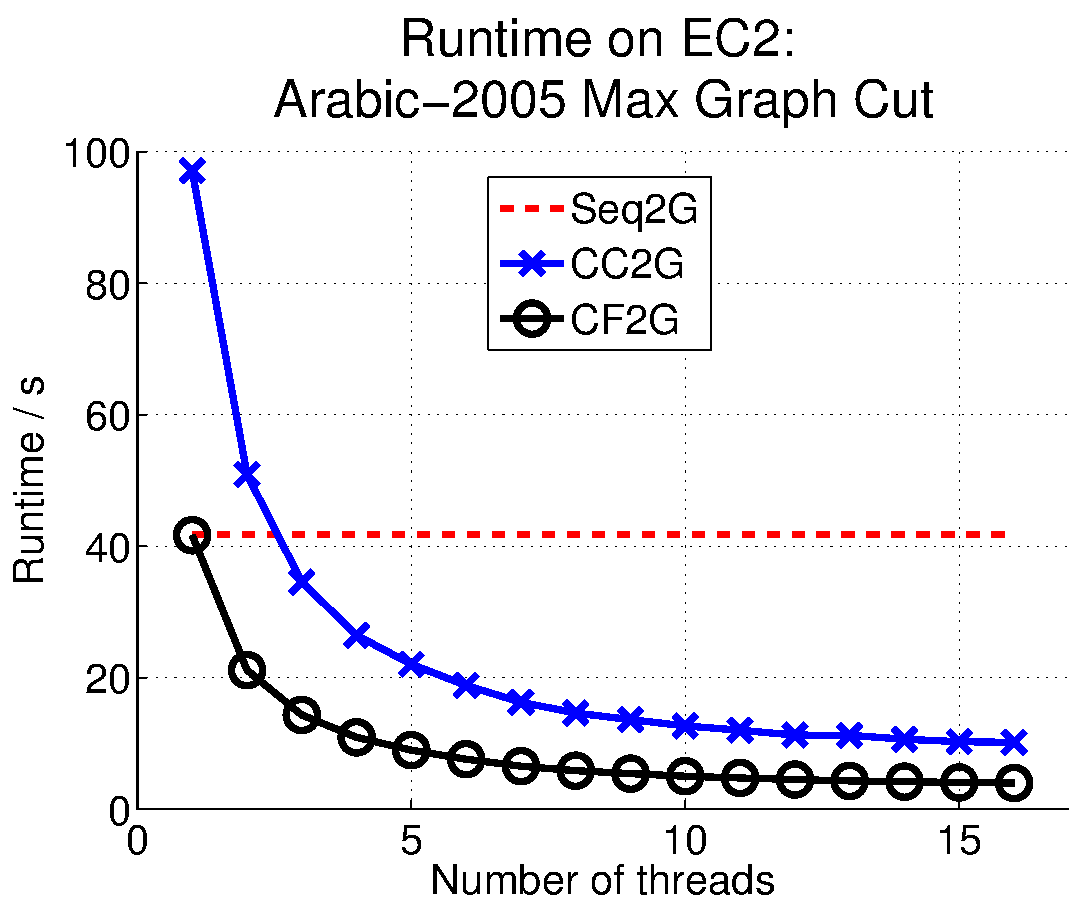
\includegraphics[width=110pt]{images/runtime_arabic2005_maxgraphcut.pdf}
			\caption{}
			\label{appfig:runtime_arabic2005_maxgraphcut}
	  \end{subfigure} &
	  \begin{subfigure}[b]{0.22\textwidth}
	  	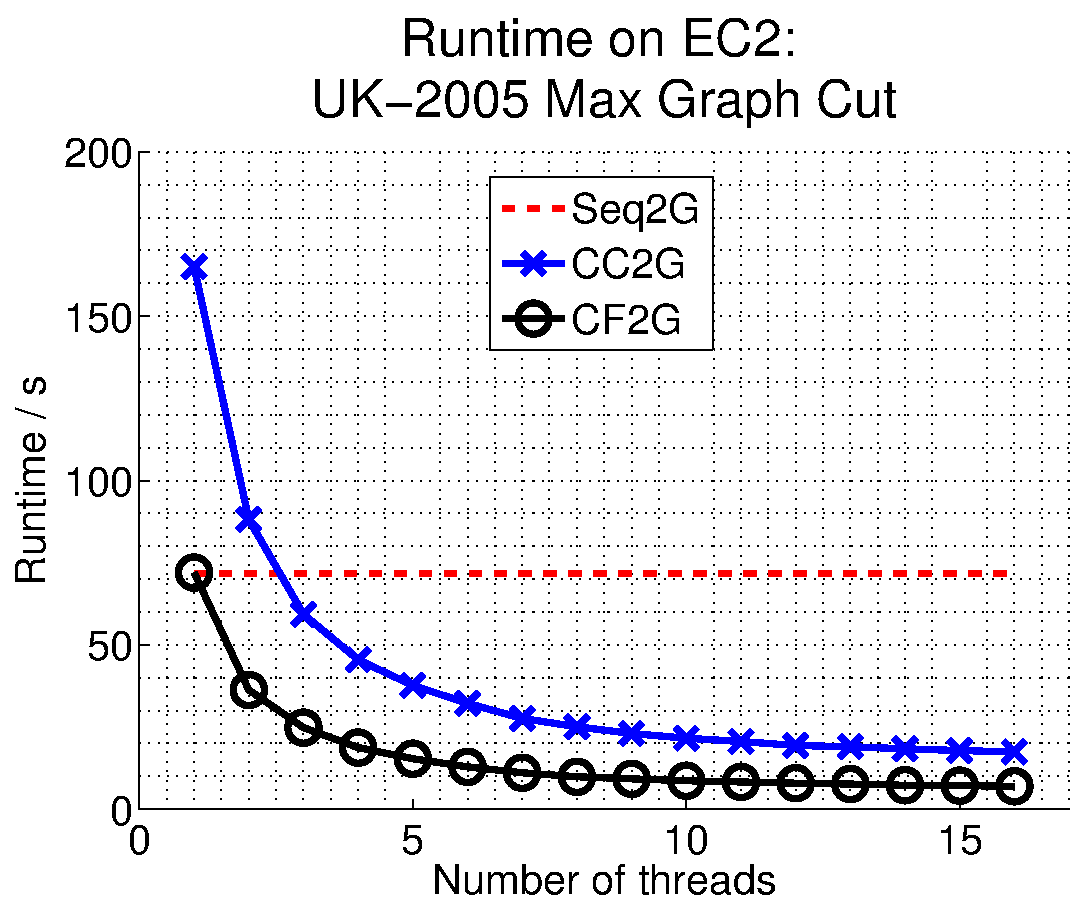
\includegraphics[width=110pt]{images/runtime_uk2005_maxgraphcut.pdf}
			\caption{}
			\label{appfig:runtime_uk2005_maxgraphcut}
	  \end{subfigure} &
	  \begin{subfigure}[b]{0.22\textwidth}
	  	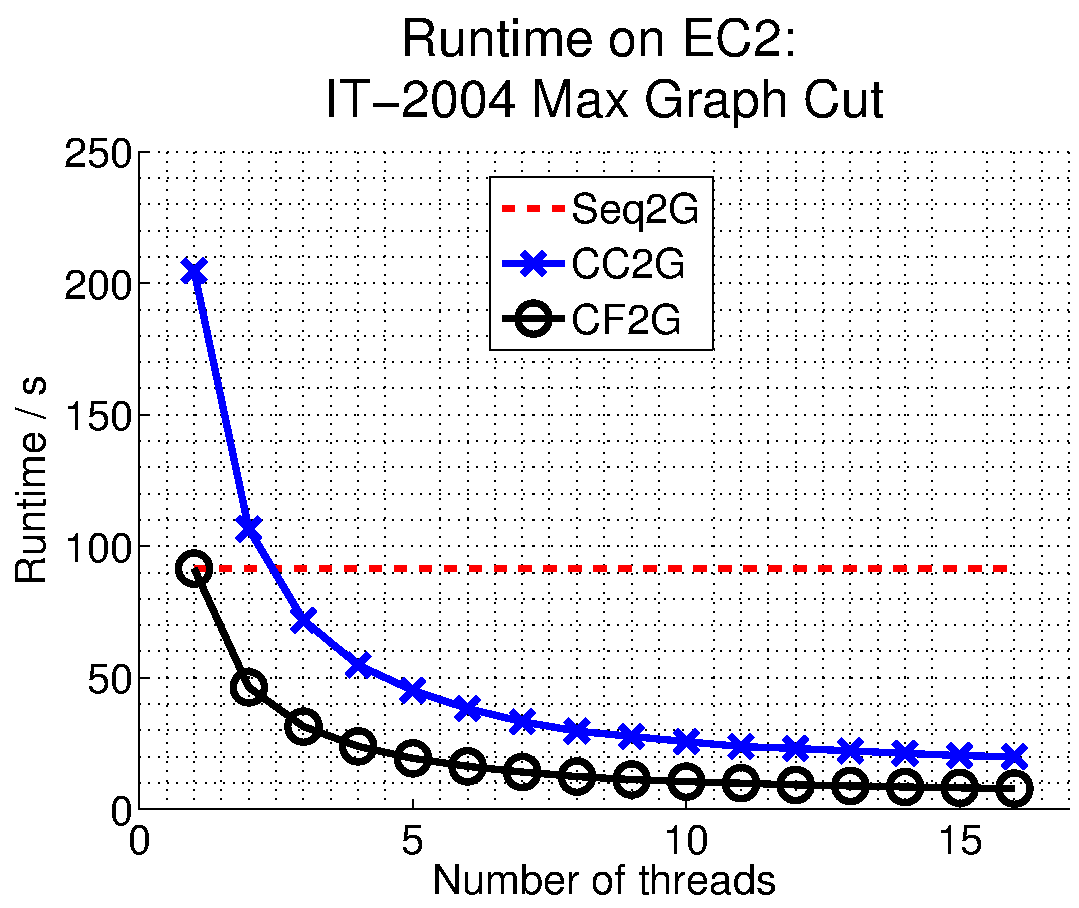
\includegraphics[width=110pt]{images/runtime_it2004_maxgraphcut.pdf}
			\caption{}
			\label{appfig:runtime_it2004_maxgraphcut}
	  \end{subfigure} \\
	  \begin{subfigure}[b]{0.22\textwidth}
	  	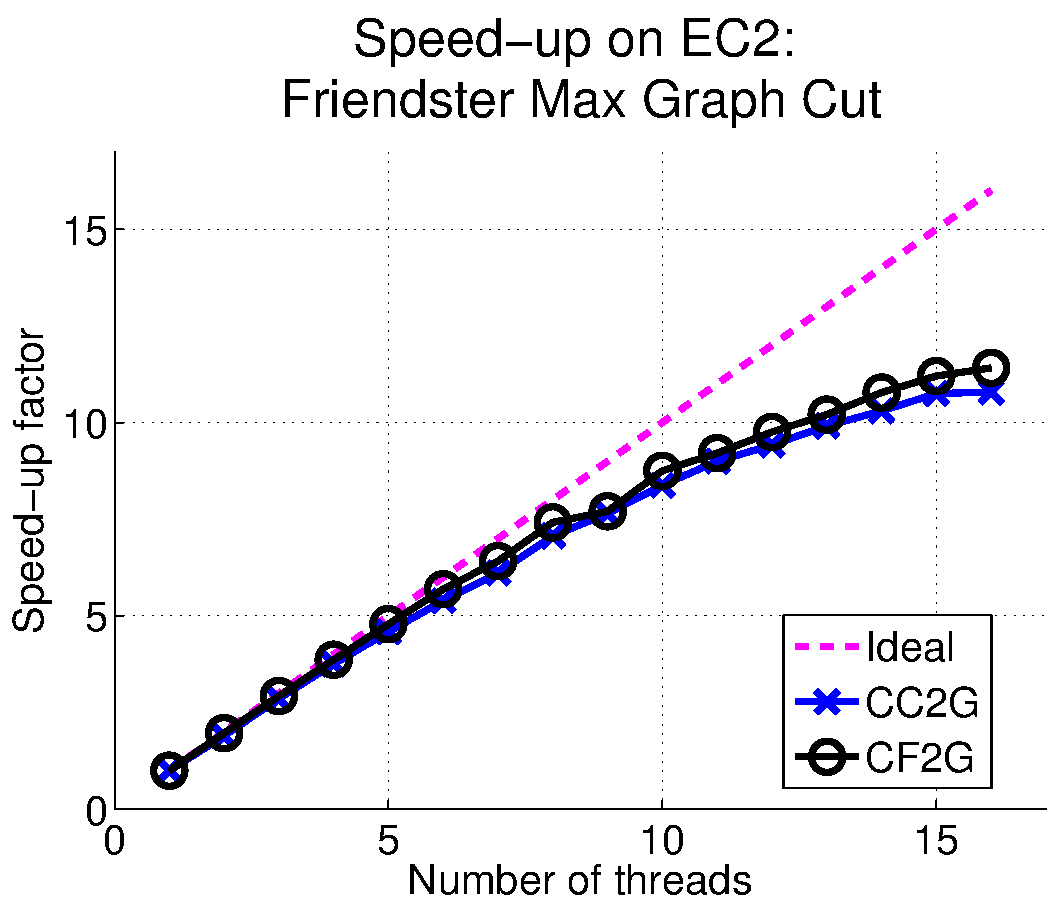
\includegraphics[width=110pt]{images/speedup_friendster10M_maxgraphcut.pdf}
			\caption{}
			\label{appfig:speedup_friendster10M_maxgraphcut}
	  \end{subfigure} &
	  \begin{subfigure}[b]{0.22\textwidth}
	  	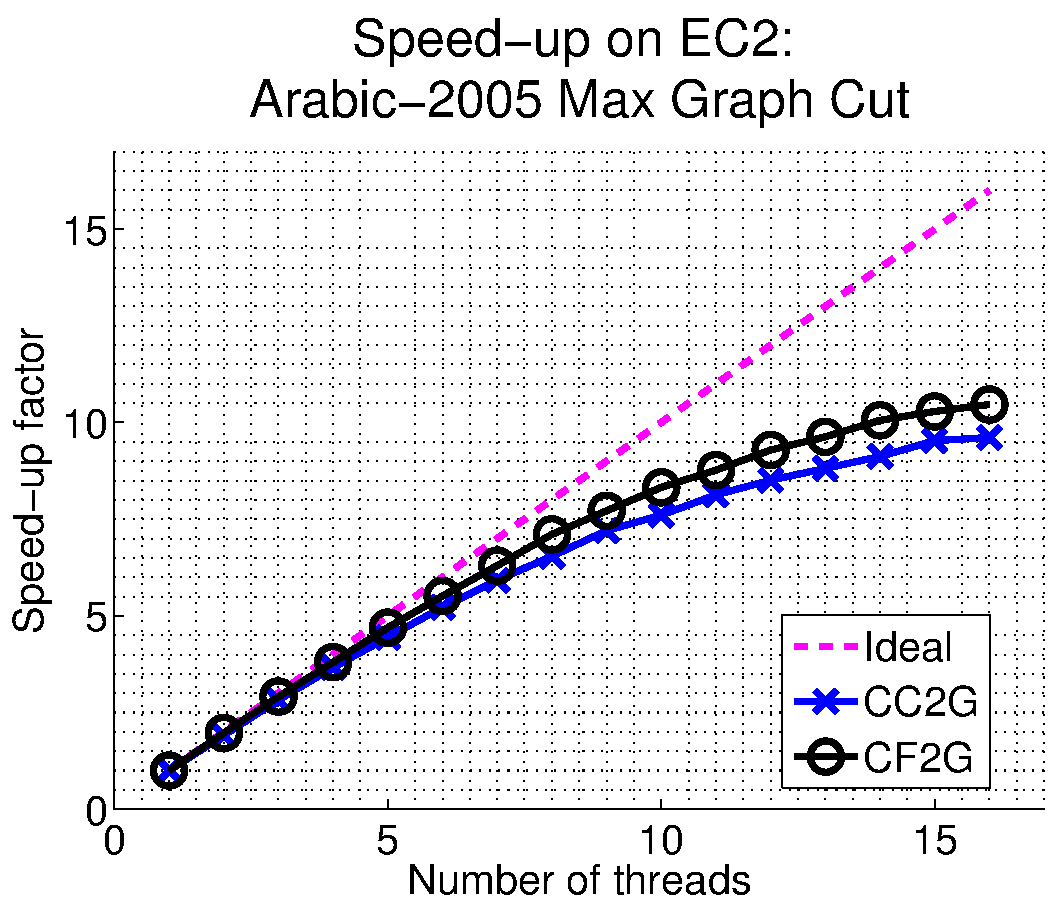
\includegraphics[width=110pt]{images/speedup_arabic2005_maxgraphcut.pdf}
			\caption{}
			\label{appfig:speedup_arabic2005_maxgraphcut}
	  \end{subfigure} &
	  \begin{subfigure}[b]{0.22\textwidth}
	  	\includegraphics[width=110pt]{images/speedup_uk2005_maxgraphcut.pdf}
			\caption{}
			\label{appfig:speedup_uk2005_maxgraphcut}
	  \end{subfigure} &
	  \begin{subfigure}[b]{0.22\textwidth}
	  	\includegraphics[width=110pt]{images/speedup_it2004_maxgraphcut.pdf}
			\caption{}
			\label{appfig:speedup_it2004_maxgraphcut}
	  \end{subfigure} \\
	  \begin{subfigure}[b]{0.22\textwidth}
	  	\includegraphics[width=110pt]{images/diffFA_CF2G_friendster10M_maxgraphcut.pdf}
			\caption{}
			\label{appfig:diffFA_CF2G_friendster10M_maxgraphcut}
	  \end{subfigure} &
	  \begin{subfigure}[b]{0.22\textwidth}
	  	\includegraphics[width=110pt]{images/diffFA_CF2G_arabic2005_maxgraphcut.pdf}
			\caption{}
			\label{appfig:diffFA_CF2G_arabic2005_maxgraphcut}
	  \end{subfigure} &
	  \begin{subfigure}[b]{0.22\textwidth}
	  	\includegraphics[width=110pt]{images/diffFA_CF2G_uk2005_maxgraphcut.pdf}
			\caption{}
			\label{appfig:diffFA_CF2G_uk2005_maxgraphcut}
	  \end{subfigure} &
	  \begin{subfigure}[b]{0.22\textwidth}
	  	\includegraphics[width=110pt]{images/diffFA_CF2G_it2004_maxgraphcut.pdf}
			\caption{}
			\label{appfig:diffFA_CF2G_it2004_maxgraphcut}
	  \end{subfigure} \\
	  \begin{subfigure}[b]{0.22\textwidth}
	  	\includegraphics[width=110pt]{images/validated_CC2G_friendster10M_maxgraphcut.pdf}
			\caption{}
			\label{appfig:validated_CC2G_friendster10M_maxgraphcut}
	  \end{subfigure} &
	  \begin{subfigure}[b]{0.22\textwidth}
	  	\includegraphics[width=110pt]{images/validated_CC2G_arabic2005_maxgraphcut.pdf}
			\caption{}
			\label{appfig:validated_CC2G_arabic2005_maxgraphcut}
	  \end{subfigure} &
	  \begin{subfigure}[b]{0.22\textwidth}
	  	\includegraphics[width=110pt]{images/validated_CC2G_uk2005_maxgraphcut.pdf}
			\caption{}
			\label{appfig:validated_CC2G_uk2005_maxgraphcut}
	  \end{subfigure} &
	  \begin{subfigure}[b]{0.22\textwidth}
	  	\includegraphics[width=110pt]{images/validated_CC2G_it2004_maxgraphcut.pdf}
			\caption{}
			\label{appfig:validated_CC2G_it2004_maxgraphcut}
	  \end{subfigure} \\
  \end{tabular}
  \caption{Max graph cut on 4 real graphs.}
\end{figure}





~\newpage\begin{figure}[ht]
  \centering
  \begin{tabular}{cccc}
	  \begin{subfigure}[h]{0.22\textwidth}
	  	\includegraphics[width=110pt]{images/runtime_ring_setcover.pdf}
			\caption{}
			\label{appfig:runtime_ring_setcover}
	  \end{subfigure} &
	  \begin{subfigure}[h]{0.22\textwidth}
	  	\includegraphics[width=110pt]{images/speedup_ring_setcover.pdf}
			\caption{}
			\label{appfig:speedup_ring_setcover}
	  \end{subfigure} &
	  \begin{subfigure}[h]{0.22\textwidth}
	  	\includegraphics[width=110pt]{images/diffFA_CF2G_ring_setcover.pdf}
			\caption{}
			\label{appfig:diffFA_CF2G_ring_setcover}
	  \end{subfigure} &
	  \begin{subfigure}[h]{0.22\textwidth}
	  	\includegraphics[width=110pt]{images/validated_CC2G_ring_setcover.pdf}
			\caption{}
			\label{appfig:validated_CC2G_ring_setcover}
	  \end{subfigure} \\
	  \begin{subfigure}[h]{0.22\textwidth}
	  	\includegraphics[width=110pt]{images/runtime_ring_maxgraphcut.pdf}
			\caption{}
			\label{appfig:runtime_ring_maxgraphcut}
	  \end{subfigure} &
	  \begin{subfigure}[h]{0.22\textwidth}
	  	\includegraphics[width=110pt]{images/speedup_ring_maxgraphcut.pdf}
			\caption{}
			\label{appfig:speedup_ring_maxgraphcut}
	  \end{subfigure} &
	  \begin{subfigure}[h]{0.22\textwidth}
	  	\includegraphics[width=110pt]{images/diffFA_CF2G_ring_maxgraphcut.pdf}
			\caption{}
			\label{appfig:diffFA_CF2G_ring_maxgraphcut}
	  \end{subfigure} &
	  \begin{subfigure}[h]{0.22\textwidth}
	  	\includegraphics[width=110pt]{images/validated_CC2G_ring_maxgraphcut.pdf}
			\caption{}
			\label{appfig:validated_CC2G_ring_maxgraphcut.pdf}
	  \end{subfigure} \\
  \end{tabular}
  \caption{\footnotesize Experimental results for ring graph on set cover problem.}
\label{appfig:results_adversarial}
\end{figure}











~\newpage\section{Full experiment results,  partitioning with work stealing}
\label{app:exptresults_partition}
\begin{figure}[ht]
  \centering
  \begin{tabular}{cccc}
	  \begin{subfigure}[b]{0.22\textwidth}
	  	\includegraphics[width=110pt]{images_partition/runtime_erdosrenyi_maxgraphcut.pdf}
			\caption{}
			\label{appfig:partition:runtime_erdosrenyi_maxgraphcut}
	  \end{subfigure} &
	  \begin{subfigure}[b]{0.22\textwidth}
	  	\includegraphics[width=110pt]{images_partition/runtime_erdosrenyi_setcover.pdf}
			\caption{}
			\label{appfig:partition:runtime_erdosrenyi_setcover}
	  \end{subfigure} &
	  \begin{subfigure}[b]{0.22\textwidth}
	  	\includegraphics[width=110pt]{images_partition/runtime_zigzag_maxgraphcut.pdf}
			\caption{}
			\label{appfig:partition:runtime_zigzag_maxgraphcut}
	  \end{subfigure} &
	  \begin{subfigure}[b]{0.22\textwidth}
	  	\includegraphics[width=110pt]{images_partition/runtime_zigzag_setcover.pdf}
			\caption{}
			\label{appfig:partition:runtime_zigzag_setcover}
	  \end{subfigure} \\
	  \begin{subfigure}[b]{0.22\textwidth}
	  	\includegraphics[width=110pt]{images_partition/speedup_erdosrenyi_maxgraphcut.pdf}
			\caption{}
			\label{appfig:partition:speedup_erdosrenyi_maxgraphcut}
	  \end{subfigure} &
	  \begin{subfigure}[b]{0.22\textwidth}
	  	\includegraphics[width=110pt]{images_partition/speedup_erdosrenyi_setcover.pdf}
			\caption{}
			\label{appfig:partition:speedup_erdosrenyi_setcover}
	  \end{subfigure} &
	  \begin{subfigure}[b]{0.22\textwidth}
	  	\includegraphics[width=110pt]{images_partition/speedup_zigzag_maxgraphcut.pdf}
			\caption{}
			\label{appfig:partition:speedup_zigzag_maxgraphcut}
	  \end{subfigure} &
	  \begin{subfigure}[b]{0.22\textwidth}
	  	\includegraphics[width=110pt]{images_partition/speedup_zigzag_setcover.pdf}
			\caption{}
			\label{appfig:partition:speedup_zigzag_setcover}
	  \end{subfigure} \\
	  \begin{subfigure}[b]{0.22\textwidth}
	  	\includegraphics[width=110pt]{images_partition/diffFA_CF2G_erdosrenyi_maxgraphcut.pdf}
			\caption{}
			\label{appfig:partition:diffFA_CF2G_erdosrenyi_maxgraphcut}
	  \end{subfigure} &
	  \begin{subfigure}[b]{0.22\textwidth}
	  	\includegraphics[width=110pt]{images_partition/diffFA_CF2G_erdosrenyi_setcover.pdf}
			\caption{}
			\label{appfig:partition:diffFA_CF2G_erdosrenyi_setcover}
	  \end{subfigure} &
	  \begin{subfigure}[b]{0.22\textwidth}
	  	\includegraphics[width=110pt]{images_partition/diffFA_CF2G_zigzag_maxgraphcut.pdf}
			\caption{}
			\label{appfig:partition:diffFA_CF2G_zigzag_maxgraphcut}
	  \end{subfigure} &
	  \begin{subfigure}[b]{0.22\textwidth}
	  	\includegraphics[width=110pt]{images_partition/diffFA_CF2G_zigzag_setcover.pdf}
			\caption{}
			\label{appfig:partition:diffFA_CF2G_zigzag_setcover}
	  \end{subfigure} \\
	  \begin{subfigure}[b]{0.22\textwidth}
	  	\includegraphics[width=110pt]{images_partition/validated_CC2G_erdosrenyi_maxgraphcut.pdf}
			\caption{}
			\label{appfig:partition:validated_CC2G_erdosrenyi_maxgraphcut}
	  \end{subfigure} &
	  \begin{subfigure}[b]{0.22\textwidth}
	  	\includegraphics[width=110pt]{images_partition/validated_CC2G_erdosrenyi_setcover.pdf}
			\caption{}
			\label{appfig:partition:validated_CC2G_erdosrenyi_setcover}
	  \end{subfigure} &
	  \begin{subfigure}[b]{0.22\textwidth}
	  	\includegraphics[width=110pt]{images_partition/validated_CC2G_zigzag_maxgraphcut.pdf}
			\caption{}
			\label{appfig:partition:validated_CC2G_zigzag_maxgraphcut}
	  \end{subfigure} &
	  \begin{subfigure}[b]{0.22\textwidth}
	  	\includegraphics[width=110pt]{images_partition/validated_CC2G_zigzag_setcover.pdf}
			\caption{}
			\label{appfig:partition:validated_CC2G_zigzag_setcover}
	  \end{subfigure} \\
  \end{tabular}
  \caption{Experimental results (with partitioning) on Erdos-Renyi and ZigZag synthetic graphs.}
\end{figure}


~\newpage\begin{figure}[ht]
  \centering
  \begin{tabular}{cccc}
	  \begin{subfigure}[b]{0.22\textwidth}
	  	\includegraphics[width=110pt]{images_partition/runtime_friendster_setcover.pdf}
			\caption{}
			\label{appfig:partition:runtime_friendster_setcover}
	  \end{subfigure} &
	  \begin{subfigure}[b]{0.22\textwidth}
	  	\includegraphics[width=110pt]{images_partition/runtime_arabic2005_setcover.pdf}
			\caption{}
			\label{appfig:partition:runtime_arabic2005_setcover}
	  \end{subfigure} &
	  \begin{subfigure}[b]{0.22\textwidth}
	  	\includegraphics[width=110pt]{images_partition/runtime_uk2005_setcover.pdf}
			\caption{}
			\label{appfig:partition:runtime_uk2005_setcover}
	  \end{subfigure} &
	  \begin{subfigure}[b]{0.22\textwidth}
	  	\includegraphics[width=110pt]{images_partition/runtime_it2004_setcover.pdf}
			\caption{}
			\label{appfig:partition:runtime_it2004_setcover}
	  \end{subfigure} \\
	  \begin{subfigure}[b]{0.22\textwidth}
	  	\includegraphics[width=110pt]{images_partition/speedup_friendster_setcover.pdf}
			\caption{}
			\label{appfig:partition:speedup_friendster_setcover}
	  \end{subfigure} &
	  \begin{subfigure}[b]{0.22\textwidth}
	  	\includegraphics[width=110pt]{images_partition/speedup_arabic2005_setcover.pdf}
			\caption{}
			\label{appfig:partition:speedup_arabic2005_setcover}
	  \end{subfigure} &
	  \begin{subfigure}[b]{0.22\textwidth}
	  	\includegraphics[width=110pt]{images_partition/speedup_uk2005_setcover.pdf}
			\caption{}
			\label{appfig:partition:speedup_uk2005_setcover}
	  \end{subfigure} &
	  \begin{subfigure}[b]{0.22\textwidth}
	  	\includegraphics[width=110pt]{images_partition/speedup_it2004_setcover.pdf}
			\caption{}
			\label{appfig:partition:speedup_it2004_setcover}
	  \end{subfigure} \\
	  \begin{subfigure}[b]{0.22\textwidth}
	  	\includegraphics[width=110pt]{images_partition/diffFA_CF2G_friendster_setcover.pdf}
			\caption{}
			\label{appfig:partition:diffFA_CF2G_friendster_setcover}
	  \end{subfigure} &
	  \begin{subfigure}[b]{0.22\textwidth}
	  	\includegraphics[width=110pt]{images_partition/diffFA_CF2G_arabic2005_setcover.pdf}
			\caption{}
			\label{appfig:partition:diffFA_CF2G_arabic2005_setcover}
	  \end{subfigure} &
	  \begin{subfigure}[b]{0.22\textwidth}
	  	\includegraphics[width=110pt]{images_partition/diffFA_CF2G_uk2005_setcover.pdf}
			\caption{}
			\label{appfig:partition:diffFA_CF2G_uk2005_setcover}
	  \end{subfigure} &
	  \begin{subfigure}[b]{0.22\textwidth}
	  	\includegraphics[width=110pt]{images_partition/diffFA_CF2G_it2004_setcover.pdf}
			\caption{}
			\label{appfig:partition:diffFA_CF2G_it2004_setcover}
	  \end{subfigure} \\
	  \begin{subfigure}[b]{0.22\textwidth}
	  	\includegraphics[width=110pt]{images_partition/validated_CC2G_friendster_setcover.pdf}
			\caption{}
			\label{appfig:partition:validated_CC2G_friendster_setcover}
	  \end{subfigure} &
	  \begin{subfigure}[b]{0.22\textwidth}
	  	\includegraphics[width=110pt]{images_partition/validated_CC2G_arabic2005_setcover.pdf}
			\caption{}
			\label{appfig:partition:validated_CC2G_arabic2005_setcover}
	  \end{subfigure} &
	  \begin{subfigure}[b]{0.22\textwidth}
	  	\includegraphics[width=110pt]{images_partition/validated_CC2G_uk2005_setcover.pdf}
			\caption{}
			\label{appfig:partition:validated_CC2G_uk2005_setcover}
	  \end{subfigure} &
	  \begin{subfigure}[b]{0.22\textwidth}
	  	\includegraphics[width=110pt]{images_partition/validated_CC2G_it2004_setcover.pdf}
			\caption{}
			\label{appfig:partition:validated_CC2G_it2004_setcover}
	  \end{subfigure} \\
  \end{tabular}
  \caption{Set cover (with partitioning) on 4 real graphs.}
\end{figure}



~\newpage\begin{figure}[ht]
  \centering
  \begin{tabular}{cccc}
	  \begin{subfigure}[b]{0.22\textwidth}
	  	\includegraphics[width=110pt]{images_partition/runtime_friendster_maxgraphcut.pdf}
			\caption{}
			\label{appfig:partition:runtime_friendster_maxgraphcut}
	  \end{subfigure} &
	  \begin{subfigure}[b]{0.22\textwidth}
	  	\includegraphics[width=110pt]{images_partition/runtime_arabic2005_maxgraphcut.pdf}
			\caption{}
			\label{appfig:partition:runtime_arabic2005_maxgraphcut}
	  \end{subfigure} &
	  \begin{subfigure}[b]{0.22\textwidth}
	  	\includegraphics[width=110pt]{images_partition/runtime_uk2005_maxgraphcut.pdf}
			\caption{}
			\label{appfig:partition:runtime_uk2005_maxgraphcut}
	  \end{subfigure} &
	  \begin{subfigure}[b]{0.22\textwidth}
	  	\includegraphics[width=110pt]{images_partition/runtime_it2004_maxgraphcut.pdf}
			\caption{}
			\label{appfig:partition:runtime_it2004_maxgraphcut}
	  \end{subfigure} \\
	  \begin{subfigure}[b]{0.22\textwidth}
	  	\includegraphics[width=110pt]{images_partition/speedup_friendster_maxgraphcut.pdf}
			\caption{}
			\label{appfig:partition:speedup_friendster_maxgraphcut}
	  \end{subfigure} &
	  \begin{subfigure}[b]{0.22\textwidth}
	  	\includegraphics[width=110pt]{images_partition/speedup_arabic2005_maxgraphcut.pdf}
			\caption{}
			\label{appfig:partition:speedup_arabic2005_maxgraphcut}
	  \end{subfigure} &
	  \begin{subfigure}[b]{0.22\textwidth}
	  	\includegraphics[width=110pt]{images_partition/speedup_uk2005_maxgraphcut.pdf}
			\caption{}
			\label{appfig:partition:speedup_uk2005_maxgraphcut}
	  \end{subfigure} &
	  \begin{subfigure}[b]{0.22\textwidth}
	  	\includegraphics[width=110pt]{images_partition/speedup_it2004_maxgraphcut.pdf}
			\caption{}
			\label{appfig:partition:speedup_it2004_maxgraphcut}
	  \end{subfigure} \\
	  \begin{subfigure}[b]{0.22\textwidth}
	  	\includegraphics[width=110pt]{images_partition/diffFA_CF2G_friendster_maxgraphcut.pdf}
			\caption{}
			\label{appfig:partition:diffFA_CF2G_friendster_maxgraphcut}
	  \end{subfigure} &
	  \begin{subfigure}[b]{0.22\textwidth}
	  	\includegraphics[width=110pt]{images_partition/diffFA_CF2G_arabic2005_maxgraphcut.pdf}
			\caption{}
			\label{appfig:partition:diffFA_CF2G_arabic2005_maxgraphcut}
	  \end{subfigure} &
	  \begin{subfigure}[b]{0.22\textwidth}
	  	\includegraphics[width=110pt]{images_partition/diffFA_CF2G_uk2005_maxgraphcut.pdf}
			\caption{}
			\label{appfig:partition:diffFA_CF2G_uk2005_maxgraphcut}
	  \end{subfigure} &
	  \begin{subfigure}[b]{0.22\textwidth}
	  	\includegraphics[width=110pt]{images_partition/diffFA_CF2G_it2004_maxgraphcut.pdf}
			\caption{}
			\label{appfig:partition:diffFA_CF2G_it2004_maxgraphcut}
	  \end{subfigure} \\
	  \begin{subfigure}[b]{0.22\textwidth}
	  	\includegraphics[width=110pt]{images_partition/validated_CC2G_friendster_maxgraphcut.pdf}
			\caption{}
			\label{appfig:partition:validated_CC2G_friendster_maxgraphcut}
	  \end{subfigure} &
	  \begin{subfigure}[b]{0.22\textwidth}
	  	\includegraphics[width=110pt]{images_partition/validated_CC2G_arabic2005_maxgraphcut.pdf}
			\caption{}
			\label{appfig:partition:validated_CC2G_arabic2005_maxgraphcut}
	  \end{subfigure} &
	  \begin{subfigure}[b]{0.22\textwidth}
	  	\includegraphics[width=110pt]{images_partition/validated_CC2G_uk2005_maxgraphcut.pdf}
			\caption{}
			\label{appfig:partition:validated_CC2G_uk2005_maxgraphcut}
	  \end{subfigure} &
	  \begin{subfigure}[b]{0.22\textwidth}
	  	\includegraphics[width=110pt]{images_partition/validated_CC2G_it2004_maxgraphcut.pdf}
			\caption{}
			\label{appfig:partition:validated_CC2G_it2004_maxgraphcut}
	  \end{subfigure} \\
  \end{tabular}
  \caption{Max graph cut (with partitioning) on 4 real graphs.}
\end{figure}





~\newpage\begin{figure}[ht]
  \centering
  \begin{tabular}{cccc}
	  \begin{subfigure}[h]{0.22\textwidth}
	  	\includegraphics[width=110pt]{images_partition/runtime_ring_setcover.pdf}
			\caption{}
			\label{appfig:partition:runtime_ring_setcover}
	  \end{subfigure} &
	  \begin{subfigure}[h]{0.22\textwidth}
	  	\includegraphics[width=110pt]{images_partition/speedup_ring_setcover.pdf}
			\caption{}
			\label{appfig:partition:speedup_ring_setcover}
	  \end{subfigure} &
	  \begin{subfigure}[h]{0.22\textwidth}
	  	\includegraphics[width=110pt]{images_partition/diffFA_CF2G_ring_setcover.pdf}
			\caption{}
			\label{appfig:partition:diffFA_CF2G_ring_setcover}
	  \end{subfigure} &
	  \begin{subfigure}[h]{0.22\textwidth}
	  	\includegraphics[width=110pt]{images_partition/validated_CC2G_ring_setcover.pdf}
			\caption{}
			\label{appfig:partition:validated_CC2G_ring_setcover}
	  \end{subfigure} \\
	  \begin{subfigure}[h]{0.22\textwidth}
	  	\includegraphics[width=110pt]{images_partition/runtime_ring_maxgraphcut.pdf}
			\caption{}
			\label{appfig:partition:runtime_ring_maxgraphcut}
	  \end{subfigure} &
	  \begin{subfigure}[h]{0.22\textwidth}
	  	\includegraphics[width=110pt]{images_partition/speedup_ring_maxgraphcut.pdf}
			\caption{}
			\label{appfig:partition:speedup_ring_maxgraphcut}
	  \end{subfigure} &
	  \begin{subfigure}[h]{0.22\textwidth}
	  	\includegraphics[width=110pt]{images_partition/diffFA_CF2G_ring_maxgraphcut.pdf}
			\caption{}
			\label{appfig:partition:diffFA_CF2G_ring_maxgraphcut}
	  \end{subfigure} &
	  \begin{subfigure}[h]{0.22\textwidth}
	  	\includegraphics[width=110pt]{images_partition/validated_CC2G_ring_maxgraphcut.pdf}
			\caption{}
			\label{appfig:partition:validated_CC2G_ring_maxgraphcut.pdf}
	  \end{subfigure} \\
  \end{tabular}
  \caption{\footnotesize Experimental results (with partitioning) for ring graph on set cover problem.}
\label{appfig:partition:results_adversarial}
\end{figure}

~


\newpage\section{Illustrative examples}

The following examples illustrate how (i) the simple (uni-directional) greedy algorithm may fail for non-monotone submodular functions, and (ii) where the coordination-free double greedy algorithm can run into trouble.

\subsection{Greedy and non-monotone functions}\label{app:greedyfail}

For illustration, consider the following toy example of a non-monotone submodular function. We are given a ground set $V = \{v_0, v_1, v_2, \ldots, v_k\}$ of $k+1$ elements, and a universe $U = \{u_1, \ldots, u_k\}$. Each element $v_i$ in $V$ covers elements $\mathrm{Cov}(v_i) \subseteq U$ of the universe. In addition, each element in $V$ has a cost $c(v_i)$. We are aiming to maximize the submodular function
\begin{equation}
  \label{eq:1}
  F(S) = |\bigcup_{v \in S}\mathrm{Cov}(v)| - \sum_{v \in S}c(v).
\end{equation}
Let the costs and coverings be as follows:
\begin{align}
  \mathrm{Cov}(v_0) &= U \qquad c(v_0) &= k-1\\
  \mathrm{Cov}(v_i) &= u_i  \qquad c(v_i) &= \epsilon \ll 1/k \text{ for all } i > 0.
\end{align}
Then the optimal solution is $S^* = V\setminus v_0$ with $FS^*) = k - k\epsilon$. 

The greedy algorithm of \citet{nemhauser1978} always adds the element with the largest marginal gain. Since $F(v_0) = 1$ and $F(v_i) = 1-\epsilon$ for all $i > 0$, the algorithm would pick $v_0$ first. After that, any additional element only has a negative marginal gain, $F(\{v_0,v_i\}) - F(v_0) = - \epsilon$. Hence, the algorithm would end up with a solution $F(v_0) = 1$ or worse.

For the double greedy algorithm, the scenario would be the following.
If $v_0$ happens to be the first element, then it picks it with probability $p(v_0) = \frac{1}{1 + k-1} = \frac{1}{k}$. If it picks $v_0$, nothing else will be added afterwards. If it does not pick $v_0$, then any other element has a probability of $\frac{1-\epsilon}{1-\epsilon} = 1$ of being added.
If $v_0$ is not the first element, then any element before $v_0$ is added with probability $p(v_i) = 1-\epsilon$, and as soon as an element $v_i$ has been picked, $v_0$ will not be added any more. Hence, with high probability, this algorithm returns the optimal solution. The deterministic version surely does.


\subsection{When is coordination needed?}



\end{document}

% This document was modified from the file originally made available by
% Pat Langley and Andrea Danyluk for ICML-2K. This version was
% created by Lise Getoor and Tobias Scheffer, it was slightly modified
% from the 2010 version by Thorsten Joachims & Johannes Fuernkranz,
% slightly modified from the 2009 version by Kiri Wagstaff and
% Sam Roweis's 2008 version, which is slightly modified from
% Prasad Tadepalli's 2007 version which is a lightly
% changed version of the previous year's version by Andrew Moore,
% which was in turn edited from those of Kristian Kersting and
% Codrina Lauth. Alex Smola contributed to the algorithmic style files.
